% !TeX root = booklet-01.tex
\clearpage
\setcounter{chapter}{-1}
\chapter{پیش‌نیازهای ریاضی، مدار و منطق دیجیتال}
\label{chap:foundations}
این فصل، پایه لازم برای خواندن درس بدون گذراندن \lr{Digital Electronics} را
فراهم می‌کند. ابتدا محاسبه و واحد، سپس قوانین مدار و در پایان منطق دیجیتال
آموزش داده می‌شود. مثال‌ها و پاسخ‌ها را به ترتیب دنبال کنید.
% !TeX root = booklet-01.tex
\section{زبان ریاضی لازم برای خواندن مدار}
\label{sec:foundation-math}
فرمول یک رابطه میان کمیت‌هاست. پیش از محاسبه باید بدانیم هر حرف چه کمیتی را
نمایش می‌دهد، واحد آن چیست و رابطه تحت چه فرضی به کار می‌رود.
در این درس، حفظ شکل رابطه بدون شناخت این سه مورد می‌تواند به جواب عددی ظاهراً درست
اما از نظر فیزیکی نامعتبر منجر شود.

\subsection{نماد، زیرنویس، کسر و نسبت}
حرفی مانند \(V\) می‌تواند نماد ولتاژ باشد؛ زیرنویس آن مشخص می‌کند کدام ولتاژ
منظور است. برای مثال، \(V_a\) ولتاژ گره \(a\) و \(V_{ab}\) اختلاف ولتاژ
گره \(a\) نسبت به \(b\) است. زیرنویس، ضرب نیست: \(V_a\) به معنی \(V\times a\) نیست.
نماد \(\Delta\) نیز تغییر کمیت را نشان می‌دهد. برای نمونه، تغییر ولتاژ را
به صورت زیر تعریف می‌کنیم.
\[
 \Delta V=V_{\mathrm{final}}-V_{\mathrm{initial}}.
\]
واژه‌های زیرنویس \(\mathrm{final}\) و \(\mathrm{initial}\) به‌ترتیب حالت نهایی و اولیه‌اند.

در کسر \(a/b\)، صورت \(a\) بر مخرج \(b\) تقسیم می‌شود و باید \(b\ne0\) باشد.
نسبت دو کمیت هم‌واحد، بدون واحد است. مثلاً نسبت \(\qty{6}{\volt}\)
به \(\qty{2}{\volt}\) برابر ۳ است؛ ولی نسبت ولتاژ به جریان واحد دارد
و می‌تواند مقاومت را بیان کند. پس واحدها بخشی از استدلال‌اند.

برای دیدن اثر یک پارامتر، نخست سایر پارامترها را ثابت می‌گیریم.
در رابطه \(y=kx\)، اگر \(k\) ثابت باشد، دو برابر شدن \(x\)، مقدار \(y\) را
دو برابر می‌کند. در \(y=k/x\)، با \(k\) ثابت و \(x\ne0\)، دو برابر شدن
\(x\)، مقدار \(y\) را نصف می‌کند. این نتیجه‌ها وقتی سایر پارامترها نیز
تغییر کنند الزاماً برقرار نیستند.

\subsection{توان و نماد علمی}
توان مثبت، ضرب تکراری است. برای پایه ده و توان سه داریم
\[
 10^3=10\times10\times10=1000.
\]
توان منفی یعنی معکوس توان مثبت. برای همان پایه و توان منفی سه داریم
\[
 10^{-3}=\frac{1}{10^3}=0.001.
\]
قواعد زیر برای پایه مثبت \(a\) و توان‌های مورد استفاده در این جزوه به کار می‌روند:
\begin{equation}\label{eq:foundation-powers}
a^m a^n=a^{m+n},\qquad
\frac{a^m}{a^n}=a^{m-n},\qquad
(a^m)^n=a^{mn}.
\end{equation}
برای نمونه، قانون تفریق توان‌ها در تقسیم می‌دهد
\[
 \frac{10^{-12}}{10^{-9}}=10^{-12-(-9)}=10^{-3}.
\]
دو علامت منفی در تفریق توان‌ها حذف می‌شوند؛ نتیجه \(10^{-21}\) نیست.

در نماد علمی، عدد را به صورت \(b\times10^n\) می‌نویسیم؛ برای عدد مثبت،
معمولاً \(1\le b<10\) است. مثلاً \(0.000024=2.4\times10^{-5}\).
در جمع، باید ابتدا توان‌ها یکسان شوند:
\[
2\times10^{-3}+3\times10^{-4}
=20\times10^{-4}+3\times10^{-4}
=23\times10^{-4}=2.3\times10^{-3}.
\]
قانون جمع توان‌ها در رابطه \eqref{eq:foundation-powers} برای ضرب است؛
به جمع دو عدد تعمیم داده نمی‌شود.

\subsection{واحد و تبدیل پیشوند}
واحدهای مورد استفاده را در جدول \ref{tab:foundation-units} می‌بینیم.
نماد واحد با نماد متغیر تفاوت دارد؛ مثلاً \(C\) متغیر ظرفیت،
ولی \(\mathrm{C}\) نماد واحد بار است.
\begin{table}[ht]
\centering
\caption{کمیت‌ها و واحدهای اصلی این بخش}
\label{tab:foundation-units}
\begin{tabular}{ccc}
\toprule
کمیت & نماد متداول & واحد \lr{SI}\\
\midrule
بار & \(Q\) & \(\mathrm{C}\)\\
جریان & \(I\) & \(\mathrm{A}\)\\
ولتاژ & \(V\) & \(\mathrm{V}\)\\
مقاومت & \(R\) & \(\Omega\)\\
ظرفیت & \(C\) & \(\mathrm{F}\)\\
زمان & \(t\) & \(\mathrm{s}\)\\
انرژی & \(E\) & \(\mathrm{J}\)\\
توان & \(P\) & \(\mathrm{W}\)\\
\bottomrule
\end{tabular}
\end{table}

پیشوندهای \lr{kilo}، \lr{milli}، \lr{micro}، \lr{nano}، \lr{pico} و
\lr{femto} به‌ترتیب ضرایب \(10^3\)، \(10^{-3}\)، \(10^{-6}\)،
\(10^{-9}\)، \(10^{-12}\) و \(10^{-15}\) هستند.
پس \(\qty{2}{\kilo\ohm}=\qty{2000}{\ohm}\) و
\(\qty{20}{\femto\farad}=20\times10^{-15}\,\mathrm{F}\).

\textbf{مثال آموزشی.} برای محاسبه زمان از نسبت بار به جریان، فرض کنید
\(Q=\qty{6}{\pico\coulomb}\) و جریان ثابت \(I=\qty{3}{\milli\ampere}\) باشد:
\begin{align*}
t&=\frac{Q}{I}
=\frac{6\times10^{-12}\,\mathrm{C}}{3\times10^{-3}\,\mathrm{A}}\\
&=2\times10^{-9}\,\mathrm{s}=\qty{2}{\nano\second}.
\end{align*}
چون \(\mathrm{A}=\mathrm{C}/\mathrm{s}\)، واحد کسر برابر ثانیه می‌شود.
این کنترل واحد، مستقل از حساب عددی است و خطای استفاده از \(I/Q\) را آشکار می‌کند.

\subsection{حل معادله با حفظ تساوی}
معادله یعنی دو عبارت مقدار یکسان دارند. برای حفظ این برابری، باید عملی یکسان
روی هر دو طرف انجام دهیم. در \(V=RI\)، برای پیدا کردن جریان و با فرض \(R\ne0\)،
دو طرف را بر \(R\) تقسیم می‌کنیم تا \(I=V/R\) به دست آید.

\textbf{مثال آموزشی.} معادله \(3x+2=11\) را حل کنیم. ابتدا از دو طرف ۲ کم
می‌کنیم و سپس دو طرف را بر ۳ تقسیم می‌کنیم.
\[
 \begin{aligned}
 3x&=9,\\
 x&=3.
 \end{aligned}
\]
جای‌گذاری در معادله اولیه می‌دهد \(3\times3+2=11\).
منظور از «انتقال جمله به طرف دیگر»، همین عمل روی دو طرف است؛ علامت‌ها بی‌دلیل تغییر نمی‌کنند.

توزیع ضرب روی پرانتز یعنی \(a(b+c)=ab+ac\).
بنابراین \(2(x-3)=2x-6\)، نه \(2x-3\).
همچنین \((x-y)^2=x^2-2xy+y^2\)؛ جمله میانی را نباید حذف کرد.
برای تقسیم بر یک عبارت حاوی مجهول، باید صفر نبودن آن را بررسی کنیم؛
تقسیم معادله \(x(x-1)=0\) بر \(x\)، جواب مجاز \(x=0\) را از دست می‌دهد.

\subsection{معادله درجه‌دو و انتخاب ریشه فیزیکی}
وقتی جمله \(x^2\) داریم، ممکن است دو جواب ریاضی وجود داشته باشد.
برای \(ax^2+bx+c=0\) با \(a\ne0\)، تعریف \(D=b^2-4ac\) می‌دهد:
\begin{equation}\label{eq:foundation-quadratic}
x=\frac{-b\pm\sqrt{D}}{2a}.
\end{equation}
در اعداد حقیقی، اگر \(D<0\) باشد جواب حقیقی نداریم؛ اگر \(D=0\)،
دو ریشه بر هم منطبق‌اند و اگر \(D>0\)، دو ریشه متمایز داریم.
نماد \(\pm\) یعنی یک‌بار علامت مثبت و یک‌بار منفی را به کار ببریم.

\textbf{مثال آموزشی بدون واحد.} فرض کنید \(x^2-3x+2=0\) و مسئله شرط
\(0\le x\le1.5\) را نیز داده باشد. در اینجا \(a=1\)، \(b=-3\) و \(c=2\) است:
\[
D=(-3)^2-4(1)(2)=1,\qquad
x=\frac{3\pm1}{2}.
\]
ریشه‌ها ۱ و ۲ هستند. هر دو معادله را ارضا می‌کنند؛ فقط ریشه ۱ در بازه مجاز است.
پس جواب مسئله ۱ است، نه صرفاً ریشه مثبت؛ هر دو ریشه در این مثال مثبت‌اند.
در تحلیل ترانزیستور نیز علاوه بر معادله، باید شرط ناحیه عملکرد و بازه ولتاژها برقرار باشد.

\subsection{خواندن نمودار و معنای شیب}
در نمودار \(y=f(x)\)، محور افقی مقدار \(x\) و محور عمودی مقدار متناظر \(y\)
را نشان می‌دهد. عبارت \(f(x)\) نام یک قانون وابستگی است؛ ضرب \(f\) در \(x\) نیست.
برای دو نقطه، شیب متوسط را تعریف می‌کنیم:
\begin{equation}\label{eq:foundation-slope}
m=\frac{y_2-y_1}{x_2-x_1},\qquad x_2\ne x_1.
\end{equation}
شیب مثبت یعنی در این بازه با افزایش \(x\)، مقدار \(y\) افزایش یافته است؛
شیب منفی یعنی کاهش یافته است. واحد شیب، واحد محور عمودی تقسیم بر واحد محور افقی است.
مثلاً اگر ولتاژ در \(\qty{2}{\nano\second}\) از صفر به \(\qty{1}{\volt}\) برسد،
شیب متوسط \(\qty{0.5}{\volt\per\nano\second}\) است.

مشتق، حد همین نسبت در یک بازه بسیار کوچک است؛ نوشتن \(\mathrm{d}V/\mathrm{d}t\)
یعنی شیب لحظه‌ای نمودار ولتاژ نسبت به زمان، نه تقسیم خود \(V\) بر خود \(t\).
برای خط راست، شیب در همه نقاط ثابت و با شیب متوسط برابر است؛ برای منحنی چنین نیست.
آموزش استخراج مشتق‌ها در محل استفاده از آن‌ها ادامه خواهد یافت.

\subsection{سنجش فهم ریاضی}
\begin{enumerate}
\item \textbf{آیا \(10^{-6}+10^{-6}=10^{-12}\) است؟}
خیر؛ مجموع \(2\times10^{-6}\) است. حاصل‌ضرب آن دو برابر \(10^{-12}\) می‌شود.
\item \textbf{در \(I=V/R\)، با ثابت بودن \(V\)، سه برابر شدن مقاومت چه اثری دارد؟}
جریان به یک‌سوم می‌رسد؛ زیرا مخرج سه برابر شده است.
\item \textbf{آیا هر ریشه‌ای که معادله را ارضا کند جواب مدار است؟}
خیر؛ باید با واحدها، بازه مجاز، اتصال‌ها و فرض‌های مدل نیز سازگار باشد.
\end{enumerate}

% !TeX root = booklet-01.tex
\section{کمیت‌های الکتریکی و خواندن اتصال‌ها}
\label{sec:foundation-circuits}
\subsection{بار، جریان و جهت مرجع}
بار الکتریکی با \(Q\) و واحد \lr{coulomb} نمایش داده می‌شود.
جریان متوسط، بار خالص عبوری از یک مقطع در واحد زمان است \cite{current}:
\begin{equation}\label{eq:foundation-current}
I_{\mathrm{avg}}=\frac{\Delta Q}{\Delta t}.
\end{equation}
برای مثال، عبور \(\qty{6}{\pico\coulomb}\) در \(\qty{2}{\nano\second}\)،
جریان متوسط \(\qty{3}{\milli\ampere}\) می‌دهد.
این رابطه از شکل تغییر جریان در طول بازه اطلاعی نمی‌دهد.
جریان لحظه‌ای با \(i(t)=\mathrm{d}Q/\mathrm{d}t\) بیان می‌شود؛ معنای نرخ تغییر
در بخش \ref{sec:foundation-math} توضیح داده شد.

جهت جریان قراردادی، جهت حرکت بار مثبت است؛ برای حرکت \lr{Electron} در فلز،
جهت حرکت حامل و جریان مخالف‌اند \cite{current}.
در تحلیل، ابتدا یک پیکان مرجع انتخاب می‌کنیم. اگر پاسخ جریان منفی شد،
جهت واقعی مخالف پیکان است؛ منفی شدن لزوماً نشانه اشتباه محاسبه نیست.

\subsection{ولتاژ، مرجع و تفاوت انرژی و توان}
ولتاژ، اختلاف پتانسیل است. تغییر انرژی پتانسیل بار مثبت \(q\) در جابه‌جایی
از نقطه \(b\) به \(a\)، برابر \(\Delta U=q(V_a-V_b)\) است.
بنابراین واحد ولتاژ، انرژی بر بار است:
\(\qty{1}{\volt}=\qty{1}{\joule\per\coulomb}\).
ولتاژ دو نقطه را با ترتیب مشخص تعریف می‌کنیم:
\begin{equation}\label{eq:foundation-voltage}
V_{ab}=V_a-V_b,\qquad V_{ba}=-V_{ab}.
\end{equation}
اگر \(V_a=\qty{1}{\volt}\) و \(V_b=\qty{0.4}{\volt}\)،
داریم \(V_{ab}=\qty{0.6}{\volt}\).
ولتاژ گره به‌تنهایی، همیشه نسبت به مرجعی مثل \lr{Ground} معنا دارد.
تغییر مرجع مشترک، اختلاف ولتاژ واقعی دو گره را تغییر نمی‌دهد.

انرژی مقدار کار قابل مبادله است؛ توان، نرخ مبادله انرژی است.
اگر جریان \(i\) وارد سر مثبت ولتاژ \(v\) یک جزء شود، توان جذب‌شده آن جزء
\(p=vi\) است. حاصل مثبت یعنی جذب و حاصل منفی یعنی تحویل انرژی به مدار.
این رابطه و کاربرد \(P=VI\) در تحلیل توان مدار با بخش \secnum{۱.۹} کتاب مرتبط‌اند
\cite{weste}. مثلاً یک مقاومت با ولتاژ \(\qty{1}{\volt}\) و جریان
\(\qty{1}{\milli\ampere}\)، توان \(\qty{1}{\milli\watt}\) جذب می‌کند؛
اگر این وضع \(\qty{2}{\milli\second}\) ثابت بماند، انرژی جذب‌شده
\(E=Pt=\qty{2}{\micro\joule}\) است. انرژی و توان هم‌واحد نیستند.

\subsection{گره، شاخه، مدار باز و اتصال کوتاه}
\lr{Node} مجموعه نقاطی است که با سیم ایدئال مستقیم متصل و هم‌پتانسیل‌اند.
وجود یک قطعه میان دو نقطه، معمولاً آن‌ها را به دو گره متفاوت تبدیل می‌کند.
\lr{Branch} یک مسیر میان دو گره است که جریان آن را در تحلیل مشخص می‌کنیم.
\lr{Ground} گره مرجع با ولتاژ صفر است؛ الزامی ندارد به زمین فیزیکی متصل باشد.

در نقشه‌های کتاب، اتصال به‌شکل \lr{T} متصل است؛ برای تقاطع دو سیم،
وجود نقطه، اتصال را مشخص می‌کند \cite[بخش \secnum{۱.۴.۲}]{weste}.
ظاهر نزدیک یا دور دو قطعه معیار هم‌گره بودن نیست؛ مسیر سیم را باید دنبال کرد.

در مدل \lr{Open Circuit}، جریان مسیر باز صفر است، ولی اختلاف ولتاژ دو سر آن
می‌تواند غیرصفر باشد. در مدل \lr{Short Circuit}، اختلاف ولتاژ صفر است؛
جریان را بقیه مدار تعیین می‌کند. اتصال کوتاه مستقیم دو سر منبع ولتاژ ایدئال
غیرصفر، مدلی ناسازگار ایجاد می‌کند؛ برای محاسبه جریان واقعی باید مقاومت‌ها و
محدودیت‌های منبع را در نظر گرفت.

\section{قوانین مدار و روش تحلیل}
\subsection{مقاومت و \lr{Ohm's Law}}
برای مقاومت خطی مثبت \(R\)، با ورود جریان مرجع به سر مثبت ولتاژ، داریم
\cite{resistors}:
\begin{equation}\label{eq:foundation-ohm}
v=Ri,\qquad i=\frac{v}{R}.
\end{equation}
مقاومت بزرگ‌تر در ولتاژ ثابت، جریان کمتری می‌دهد.
اگر جریان محاسبه‌شده منفی شود، جهت مرجع برعکس جریان واقعی بوده است.
از \(p=vi\) و رابطه \eqref{eq:foundation-ohm} نتیجه می‌گیریم
\(p=Ri^2=v^2/R\ge0\). پس مقاومت مثبت در این مدل انرژی تولید نمی‌کند.
ترانزیستور را نباید در تمام ناحیه‌های عملکرد، یک مقاومت ثابت فرض کرد؛
رابطه جریان آن در ادامه جزوه استخراج خواهد شد.

\subsection{قانون گره: \lr{KCL}}
در مدل مدار متمرکز، با حساب‌کردن جریان تمام شاخه‌ها از جمله شاخه‌های خازنی،
مجموع جریان‌های ورودی به گره با مجموع جریان‌های خروجی برابر است
\cite{kirchhoff}. این قانون با نام \lr{Kirchhoff's Current Law (KCL)} شناخته می‌شود:
\begin{equation}\label{eq:foundation-kcl}
\sum I_{\mathrm{in}}=\sum I_{\mathrm{out}}.
\end{equation}
نماد \(\sum\) یعنی جمع‌کردن همه جمله‌های مربوط.
مثلاً اگر \(\qty{3}{\milli\ampere}\) وارد گره و
\(\qty{1}{\milli\ampere}\) از یک شاخه خارج شود، جریان خروجی شاخه دیگر
\(\qty{2}{\milli\ampere}\) است. اگر خروجی به خازن متصل باشد، نباید
جریان شارژ آن را از معادله حذف کنیم.

\subsection{قانون حلقه: \lr{KVL}}
در تحلیل مدار متمرکز و با صرف‌نظر از القای مغناطیسی مدل‌نشده، جمع جبری تغییرات
ولتاژ در پیمودن یک مسیر بسته صفر است \cite{kirchhoff}.
این \lr{Kirchhoff's Voltage Law (KVL)} است:
\begin{equation}\label{eq:foundation-kvl}
\sum_{\mathrm{loop}}\Delta V=0.
\end{equation}
در عبور از منبع از پایانه منفی به مثبت، افزایش ولتاژ داریم؛ در عبور از مقاومت
در جهت جریان، افت \(IR\) داریم. مثلاً منبع \(V_s\) و دو مقاومت سری می‌دهند
\(V_s-IR_1-IR_2=0\). از اینجا
\(I=V_s/(R_1+R_2)\) به دست می‌آید. جهت پیمودن حلقه دلخواه است؛
باید علامت‌ها با همان انتخاب سازگار بمانند.

\subsection{اتصال \lr{Series} و \lr{Parallel} را از گره‌ها بشناسیم}
دو مقاومت وقتی سری‌اند که گره مشترکشان شاخه دیگری نداشته باشد؛ جریان یکسانی از
هر دو می‌گذرد. از جمع افت ولتاژها، \(R_{\mathrm{eq}}=R_1+R_2\) نتیجه می‌شود.
وقتی دو مقاومت دقیقاً میان دو گره یکسان باشند، موازی‌اند و ولتاژ یکسانی دارند.
با جمع جریان‌ها طبق \lr{KCL} به دست می‌آید \cite{resistors}:
\begin{align}
I&=\frac{V}{R_1}+\frac{V}{R_2}
=V\left(\frac{1}{R_1}+\frac{1}{R_2}\right),\notag\\
\frac{1}{R_{\mathrm{eq}}}&=\frac{1}{R_1}+\frac{1}{R_2},
\qquad R_{\mathrm{eq}}=\frac{R_1R_2}{R_1+R_2}.
\label{eq:foundation-parallel}
\end{align}
برای دو مقاومت مثبت، مقاومت معادل موازی از هر دو کمتر است؛ این یک کنترل مفید برای جواب است.
مثلاً دو مقاومت \(\qty{2}{\kilo\ohm}\) و \(\qty{3}{\kilo\ohm}\)،
در سری \(\qty{5}{\kilo\ohm}\) و در موازی \(\qty{1.2}{\kilo\ohm}\) می‌دهند.

\subsection{مثال کامل: استخراج ولتاژ یک گره}
در شکل \ref{fig:foundation-divider}، منبع ایدئال \(V_s\) و دو مقاومت مثبت داریم.
خروجی بار رسانشی ندارد. شکل برای همین جزوه رسم شده است.
\begin{figure}[ht]
\centering
\begin{latin}
\begin{circuitikz}[american]
\draw (0,0) node[ground] {} to[V,invert,l=$V_s$] (0,3)
 to[R,l=$R_1$] (3,3) to[R,l=$R_2$] (3,0) -- (0,0);
\draw (3,3) to[short,*-o] (4.7,3) node[right] {$V_x$};
\end{circuitikz}
\end{latin}
\caption{مدار آموزشی تقسیم ولتاژ؛ خروجی از گره مشترک دو مقاومت گرفته می‌شود.}
\label{fig:foundation-divider}
\end{figure}
جریان \(R_1\) را از منبع به گره \(x\) و جریان \(R_2\) را از گره به زمین
انتخاب می‌کنیم. ولتاژهای دو سر مقاومت‌ها به‌ترتیب \(V_s-V_x\) و \(V_x-0\) هستند.
با استفاده از \lr{Ohm's Law} و سپس \lr{KCL}:
\begin{align}
\frac{V_s-V_x}{R_1}&=\frac{V_x}{R_2},\notag\\
R_2(V_s-V_x)&=R_1V_x,\notag\\
R_2V_s&=(R_1+R_2)V_x,\notag\\
V_x&=V_s\frac{R_2}{R_1+R_2}.
\label{eq:foundation-divider}
\end{align}
در سطر دوم دو طرف را در \(R_1R_2\) ضرب کردیم؛ سپس پرانتز را باز و جمله‌های
حاوی \(V_x\) را یک طرف جمع کردیم. با \(V_s=\qty{1}{\volt}\)،
\(R_1=\qty{2}{\kilo\ohm}\) و \(R_2=\qty{3}{\kilo\ohm}\)،
داریم \(V_x=\qty{0.6}{\volt}\).
جریان هر دو مقاومت \(\qty{0.2}{\milli\ampere}\) و افت‌ها
\(\qty{0.4}{\volt}\) و \(\qty{0.6}{\volt}\) هستند؛ جمع افت‌ها با منبع برابر است.

\textbf{کنترل حدی و فرض بار.} با میل \(R_2\) به صفر، خروجی به صفر و با
بسیار بزرگ شدن آن نسبت به \(R_1\)، خروجی به \(V_s\) نزدیک می‌شود.
اگر بار مقاومتی \(R_L\) از خروجی به زمین وصل شود، در رابطه
\eqref{eq:foundation-divider} باید \(R_2\) را با \(R_2\parallel R_L\) جایگزین کرد؛
زیرا دیگر جریان \(R_1\) فقط از \(R_2\) نمی‌گذرد. نماد \(\parallel\) اتصال موازی را نشان می‌دهد.

\section{خازن، شارژ و مفهوم زمان}
\label{sec:foundation-capacitor}
\subsection{خازن چه چیزی را ذخیره می‌کند؟}
خازن از دو رسانا با ماده عایق میان آن‌ها ساخته می‌شود.
در مدل دوصفحه‌ای ایدئال، بارهای صفحات \(+Q\) و \(-Q\) هستند؛
مجموع بار دو صفحه می‌تواند صفر باشد، درحالی‌که انرژی در میدان ذخیره شده است
\cite{capacitors}. پس عبارت «بار خازن» معمولاً به بار علامت‌دار یک صفحه
یا اندازه بار صفحات اشاره دارد، نه مجموع آن دو.

اگر ظرفیت ثابت \(C\) باشد و \(v\) را ولتاژ صفحه اول نسبت به دوم بگیریم،
بار صفحه اول برابر است با:
\begin{equation}\label{eq:foundation-qcv}
Q=Cv,\qquad C=\frac{Q}{v}\quad(v\ne0).
\end{equation}
واحد ظرفیت \lr{farad} است و \(\mathrm{F}=\mathrm{C}/\mathrm{V}\).
مثلاً در خازن \(\qty{20}{\femto\farad}\)، ولتاژ \(\qty{1}{\volt}\)
با بار \(\qty{20}{\femto\coulomb}\) روی صفحه مثبت همراه است.
ظرفیت بزرگ‌تر در ولتاژ یکسان، بار بیشتری لازم دارد.

\subsection{از تغییر بار به تغییر ولتاژ}
برای ظرفیت ثابت، از رابطه \eqref{eq:foundation-qcv} داریم
\(\Delta Q=C\Delta v\). تقسیم دو طرف بر \(\Delta t\) و استفاده از تعریف
جریان متوسط می‌دهد:
\begin{equation}\label{eq:foundation-cap-current}
I_{\mathrm{avg}}=C\frac{\Delta v}{\Delta t},
\qquad i(t)=C\frac{\mathrm{d}v}{\mathrm{d}t}.
\end{equation}
در این قرارداد، جریان وارد صفحه‌ای می‌شود که ولتاژ مثبت برای آن تعریف شده است.
جریان مثبت بار آن صفحه و ولتاژ آن را افزایش می‌دهد؛ جریان منفی کاهش می‌دهد.
رابطه دوم شکل لحظه‌ای همان رابطه اول است. این ارتباط مبنای توضیح زمان تغییر خروجی
در کتاب و اسلاید است \cite[بخش \secnum{۱.۹}]{weste}\cite[اسلاید ۸]{mos}.
برای ظرفیت وابسته به ولتاژ، باید به رابطه عمومی \(i=\mathrm{d}Q/\mathrm{d}t\)
برگردیم؛ ثابت گرفتن \(C\) یک فرض مدل است.

\textbf{مثال آموزشی.} فرض کنیم جریان خالص ثابت \(I=\qty{10}{\micro\ampere}\)
به خازن \(C=\qty{20}{\femto\farad}\) وارد شود و ولتاژ آن از
\(\qty{0.2}{\volt}\) به \(\qty{0.8}{\volt}\) برسد. تغییر ولتاژ
\(\Delta v=\qty{0.6}{\volt}\) است. پس:
\begin{align}
\Delta t&=\frac{C\Delta v}{I}
=\frac{(20\times10^{-15}\,\mathrm{F})(0.6\,\mathrm{V})}
{10\times10^{-6}\,\mathrm{A}}\notag\\
&=1.2\times10^{-9}\,\mathrm{s}=\qty{1.2}{\nano\second}.
\label{eq:foundation-charge-time}
\end{align}
واحد \(\mathrm{F}\,\mathrm{V}/\mathrm{A}\) برابر ثانیه است.
در این مدل، دو برابر شدن ظرفیت، زمان را دو برابر و دو برابر شدن جریان، زمان را نصف می‌کند.
این نتیجه برای جریان ثابت است؛ جریان ترانزیستور واقعی عموماً طی تغییر ولتاژ ثابت نیست.

\subsection{حالت ماندگار، گذرا و پاسخ ساده \lr{RC}}
در حالت ماندگار \lr{DC}، ولتاژ خازن ثابت است؛ بنابراین در مدل ایدئال
\(\mathrm{d}v/\mathrm{d}t=0\) و جریان آن صفر می‌شود. این به معنی صفر بودن ولتاژ آن نیست.
در حالت گذرا، بار و ولتاژ تغییر می‌کنند. اختلاف ولتاژ خازن در حضور جریان محدود
نمی‌تواند ناگهان جهش کند؛ چون جهش نیازمند انتقال بار محدود در زمان صفر است.

برای درک تفاوت با جریان ثابت، خازنی را در نظر بگیرید که از منبع ثابت \(V_s\)
از طریق مقاومت \(R\) شارژ می‌شود؛ بار دیگری وجود ندارد و \(v(0)=0\).
با افزایش ولتاژ خازن، اختلاف ولتاژ مقاومت کم می‌شود؛ در نتیجه جریان
\(i=(V_s-v)/R\) کاهش می‌یابد. پس نمودار ولتاژ خط راست نیست.
از \lr{KCL} و رابطه \eqref{eq:foundation-cap-current} به دست می‌آید:
\begin{equation}\label{eq:foundation-rc-ode}
C\frac{\mathrm{d}v}{\mathrm{d}t}=\frac{V_s-v}{R}.
\end{equation}
جواب زیر فعلاً برای تفسیر معرفی می‌شود؛ می‌توان درستی آن را با مشتق‌گیری کنترل کرد:
\begin{equation}\label{eq:foundation-rc}
v(t)=V_s\left(1-e^{-t/(RC)}\right),\qquad t\ge0.
\end{equation}
عدد \(e\approx2.718\) پایه تابع نمایی است. برای عدد بی‌بعد مثبت \(x\)،
\(e^{-x}=1/e^x\)؛ با بزرگ شدن \(x\)، این مقدار به صفر نزدیک می‌شود.
حاصل \(RC\) واحد زمان دارد و آن را ثابت زمانی \(\tau=RC\) می‌نامیم.
در \(t=0\)، جواب صفر است؛ در \(t=\tau\)، مقدار ولتاژ تقریباً
\(0.632V_s\) و با زیاد شدن زمان، حد آن \(V_s\) است.
در مدل ایدئال نمایی، رسیدن دقیق به حد در زمان محدود رخ نمی‌دهد.

شکل \ref{fig:foundation-rc} همین پاسخ را بدون وابستگی به مقیاس یک فناوری
نشان می‌دهد. محور افقی زمان تقسیم بر ثابت زمانی و محور عمودی ولتاژ تقسیم بر
ولتاژ منبع است؛ هر دو نسبت بدون واحدند. کم‌شدن شیب یعنی کاهش جریان شارژ.
\begin{figure}[ht]
\centering
\begin{latin}
\begin{tikzpicture}[x=1.6cm,y=2.6cm]
\draw[->] (0,0) -- (3.6,0) node[right] {$t/\tau$};
\draw[->] (0,0) -- (0,1.25) node[above] {$v/V_s$};
\draw[dashed] (0,1) -- (3.3,1);
\node[left] at (0,1) {\rl{۱}};
\node[below left] at (0,0) {\rl{۰}};
\foreach \x/\ticklabel in {1/۱,2/۲,3/۳} {\draw (\x,0.025) -- (\x,-0.025) node[below] {\rl{\ticklabel}};}
\draw[thick,domain=0:3.3,samples=70] plot (\x,{1-exp(-\x)});
\draw[dotted] (1,0) -- (1,{1-exp(-1)}) -- (0,{1-exp(-1)});
\fill (1,{1-exp(-1)}) circle (1.4pt);
% Match the shared digit font for the Persian decimal separator.
\node[left] at (0,{1-exp(-1)}) {\fontspec[Path=C:/Windows/Fonts/]{arial.ttf}\mbox{\beginL۰٫۶۳۲\endL}};
\end{tikzpicture}
\end{latin}
\caption{نمودار تحلیلی پاسخ \lr{RC} رابطه \eqref{eq:foundation-rc}؛
این شکل از خود رابطه رسم شده است و نتیجه شبیه‌سازی \lr{SPICE} نیست.}
\label{fig:foundation-rc}
\end{figure}

برای دیدن سازگاری جواب با معادله، پاسخ و مشتق آن را کنار هم می‌نویسیم.
\[
 \begin{aligned}
 v&=V_s(1-e^{-t/\tau}),\\
 \frac{\mathrm{d}v}{\mathrm{d}t}&=\frac{V_s}{\tau}e^{-t/\tau}.
 \end{aligned}
\]
پس دو طرف رابطه \eqref{eq:foundation-rc-ode} برابر
\((V_s/R)e^{-t/\tau}\) می‌شوند. قاعده مشتق نمایی در اینجا معرفی شده است؛
استخراج تفصیلی قواعد مشتق در محل نیاز بعدی آموزش داده می‌شود.

\subsection{پرسش‌های مدار با پاسخ}
\begin{enumerate}
\item \textbf{در تقسیم ولتاژ با دو مقاومت مساوی و خروجی بی‌بار، خروجی چقدر است؟}
نصف منبع؛ زیرا \(R/(R+R)=1/2\). این حکم برای خروجی بارگذاری‌شده الزاماً برقرار نیست.
\item \textbf{اگر ولتاژ یک خازن ایدئال ثابت باشد، چه چیزی درباره جریان می‌دانیم؟}
جریان خازن صفر است، ولی شاخه‌های دیگر مدار می‌توانند جریان غیرصفر داشته باشند.
\item \textbf{چرا مدل جریان ثابت و مدل شارژ مقاومتی دو نمودار متفاوت می‌دهند؟}
در اولی شیب \(I/C\) ثابت است؛ در دومی جریان با افزایش ولتاژ خازن کاهش می‌یابد.
\item \textbf{اگر جواب جریان یک مقاومت منفی شد، چه کنیم؟}
ابتدا جهت مرجع و قطب‌های ولتاژ را کنترل کنیم؛ اگر معادله‌ها سازگار باشند،
علامت منفی فقط جهت مخالف جریان واقعی را نشان می‌دهد.
\end{enumerate}

% !TeX root = booklet-01.tex
\section{از ولتاژ فیزیکی به منطق دیجیتال}
\subsection{چرا مقدار منطقی با ولتاژ یکی نیست؟}
سیگنال فیزیکی مدار، ولتاژ یا جریان است؛ مدل دیجیتال بخشی از این رفتار را با
مقادیر گسسته صفر و یک توصیف می‌کند. سیگنال \lr{Analog} می‌تواند در یک بازه
مقادیر پیوسته داشته باشد؛ در توصیف \lr{Digital}، بازه‌هایی از ولتاژ به مقدارهای
منطقی نگاشت می‌شوند. خود ولتاژ واقعی مدار دیجیتال نیز هنگام تغییر پیوسته است.
در قرارداد این درس، ولتاژ نزدیک \lr{Ground} نماینده صفر و نزدیک
\(V_{\mathrm{DD}}\) نماینده یک است \cite[بخش \secnum{۱.۳}]{weste}.
نماد \(V_{\mathrm{DD}}\) نام ریل تغذیه مثبت است، نه یک مقدار ثابت همگانی.

\textbf{مثال آموزشی با مرزهای فرضی.} فرض کنید در مداری با تغذیه
\(\qty{1}{\volt}\)، ورودی از صفر تا \(\qty{0.3}{\volt}\) صفر معتبر و
از \(\qty{0.7}{\volt}\) تا تغذیه یک معتبر تعریف شود.
ولتاژ \(\qty{0.2}{\volt}\) صفر معتبر است، هرچند صفر ولت نیست؛
\(\qty{0.8}{\volt}\) یک معتبر و \(\qty{0.5}{\volt}\) در بازه نامعین است.
این مرزها صرفاً برای آموزش‌اند و مشخصات یک فناوری واقعی را بیان نمی‌کنند.
سطح‌های معتبر و \NotesTopic{sec:noise-margin}{\lr{Noise Margin}} از
مشخصه انتقال مدار استخراج می‌شوند.

\subsection{بیت، بردار و شمارش حالت‌ها}
یک \lr{Bit} یک مقدار دودویی دارد. دو بیت مستقل چهار ترکیب و \(n\) بیت مستقل
\(2^n\) ترکیب دارند؛ هر بیت تعداد حالت‌ها را دو برابر می‌کند.
برای سه ورودی، بنابراین هشت سطر در جدول کامل نیاز داریم.
برای آشنایی با نمایش عددی، سه بیت \(b_2,b_1,b_0\) در نمایش بدون علامت، عدد
\(4b_2+2b_1+b_0\) را نمایش می‌دهند. مثلاً بیت‌های ۱، ۰، ۱ مقدار ۵ دارند.
اما هر بردار منطقی الزاماً عدد نیست؛ می‌تواند سه سیگنال کنترل مستقل باشد.

\section{گیت‌های پایه و \lr{Truth Table}}
\subsection{تعریف عملگرها و ترتیب محاسبه}
\lr{Truth Table} خروجی را برای تمام ترکیب‌های مجاز ورودی می‌نویسد.
در این بخش ورودی‌ها فقط صفر یا یک هستند.
\lr{NOT} مقدار را معکوس می‌کند؛ آن را با خط بالای متغیر می‌نویسیم:
\(\overline{0}=1\) و \(\overline{1}=0\).
این خط علامت منفی عددی نیست.

عملگر \lr{AND} فقط وقتی یک است که همه ورودی‌ها یک باشند؛ نماد آن
\(A\cdot B\) یا \(AB\) است.
عملگر \lr{OR} وقتی یک است که دست‌کم یک ورودی یک باشد؛ نماد آن \(A+B\) است.
در اینجا \(+\) جمع معمولی نیست: \(1+1=1\) در جبر منطقی.
\lr{XOR} برای دو ورودی وقتی یک است که ورودی‌ها متفاوت باشند و با
\(A\oplus B\) نمایش داده می‌شود. \lr{NAND}، \lr{NOR} و \lr{XNOR}
به‌ترتیب مکمل \lr{AND}، \lr{OR} و \lr{XOR} هستند.
این تعریف‌ها زمینه خواندن گیت‌های بخش \secnum{۱.۴} کتاب را فراهم می‌کنند \cite{weste}.

جدول \ref{tab:foundation-gates} تمام حالت‌های دو ورودی را نشان می‌دهد.
برای جلوگیری از ابهام، در روابط ترکیبی از پرانتز استفاده می‌کنیم؛
در قرارداد متعارف، \lr{NOT} پیش از \lr{AND} و سپس \lr{OR} محاسبه می‌شود.
\begin{table}[ht]
\centering
\caption{جدول گیت‌های دوورودی؛ همه مدخل‌ها مقدار منطقی بدون واحد هستند.}
\label{tab:foundation-gates}
\begin{tabular}{cccccccc}
\toprule
\(A\)&\(B\)&\lr{AND}&\lr{OR}&\lr{XOR}&\lr{NAND}&\lr{NOR}&\lr{XNOR}\\
\midrule
۰&۰&۰&۰&۰&۱&۱&۱\\
۰&۱&۰&۱&۱&۱&۰&۰\\
۱&۰&۰&۱&۱&۱&۰&۰\\
۱&۱&۱&۱&۰&۰&۰&۱\\
\bottomrule
\end{tabular}
\end{table}
برای مثال، در سطر آخر، \lr{OR} یک ولی \lr{XOR} صفر است؛
پس «یا»ی \lr{OR} حالت هم‌زمان یک بودن هر دو ورودی را حذف نمی‌کند.

\subsection{مثال مرحله‌ای و ساخت جدول از عبارت}
برای عبارت \(Y=\overline{AB+C}\)، ابتدا \(AB\)، سپس \(AB+C\) و در پایان
مکمل کل عبارت را محاسبه می‌کنیم. با \(A=1\)، \(B=0\) و \(C=1\)،
داریم \(AB=0\)، سپس \(0+1=1\) و در نتیجه \(Y=0\).
خط مکمل فقط روی \(C\) نیست؛ محل و طول آن جزئی از تعریف تابع است.

برای ساخت جدول کامل، هر هشت ترکیب ورودی را می‌نویسیم و ستون میانی \(AB\)
را پیش از \(Y\) محاسبه می‌کنیم. راه فشرده‌تر برای فهم نتیجه این است:
اگر \(C=1\)، خروجی در همه حالت‌ها صفر است؛ اگر \(C=0\)،
داریم \(Y=\overline{AB}\). پس خروجی فقط در سه حالت
\((A,B,C)=(0,0,0),(0,1,0),(1,0,0)\) یک است.
این نتیجه با تعریف \lr{NAND} در جدول \ref{tab:foundation-gates} قابل کنترل است.

\subsection{از جدول به عبارت منطقی}
اگر خروجی تابعی فقط برای دو حالت \((A,B)=(0,1)\) و \((1,0)\) یک باشد،
برای حالت اول عبارت \(\overline{A}B\) و برای حالت دوم \(A\overline{B}\) را می‌نویسیم.
هر عبارت فقط همان حالت خود را تشخیص می‌دهد. سپس آن‌ها را با \lr{OR} ترکیب می‌کنیم:
\begin{equation}\label{eq:foundation-xor}
Y=\overline{A}B+A\overline{B}=A\oplus B.
\end{equation}
بنابراین جدول، عبارت و شبکه گیت‌ها سه نمایش مرتبط از یک تابع‌اند.
برای تعداد ورودی زیاد، روش‌های ساده‌سازی کارآمدتری وجود دارد؛
در این بخش هدف فهم نگاشت میان این نمایش‌هاست.

\section{جبر منطقی و اتصال \lr{Switch}ها}
\subsection{قانون‌های موردنیاز و کنترل آن‌ها}
برای متغیر دودویی \(A\)، روابط زیر از بررسی دو مقدار صفر و یک به دست می‌آیند:
\begin{align}
A+0&=A,& A\cdot1&=A,& A+1&=1,& A\cdot0&=0,\notag\\
A+A&=A,& AA&=A,& A+\overline{A}&=1,& A\overline{A}&=0.
\label{eq:foundation-identities}
\end{align}
مثلاً \(A+A=A\) نشان می‌دهد نباید جمع منطقی را مانند جمع عددی
به \(2A\) تبدیل کنیم.
دو قانون پرکاربرد دیگر، توزیع \(A(B+C)=AB+AC\) و جذب
\(A+AB=A\) هستند. برای جذب، اگر \(A=1\)، خروجی در هر صورت یک است؛
اگر \(A=0\)، هر دو جمله صفرند. پس دو طرف در همه حالت‌ها برابرند.

\lr{De Morgan's Laws} می‌گویند مکمل \lr{AND} برابر \lr{OR} مکمل‌ها و
مکمل \lr{OR} برابر \lr{AND} مکمل‌هاست \cite[بخش \secnum{۱.۴}]{weste}:
\begin{equation}\label{eq:foundation-demorgan}
\overline{AB}=\overline{A}+\overline{B},\qquad
\overline{A+B}=\overline{A}\,\overline{B}.
\end{equation}
برای رابطه اول، خروجی فقط وقتی صفر است که هر دو ورودی یک باشند؛
در غیر این صورت حداقل یک مکمل، یک است. این استدلال تمام چهار حالت را پوشش می‌دهد.
پس هنگام بردن مکمل داخل پرانتز، هم متغیرها مکمل می‌شوند و هم عملگر عوض می‌شود.

\textbf{مثال آموزشی.} با جذب داریم
\[
 F=A+\overline{A}B=(A+\overline{A})(A+B)=A+B.
\]
در این تبدیل از قانون توزیع دیگر جبر منطقی،
\(X+YZ=(X+Y)(X+Z)\)، استفاده شده است.
می‌توان بدون حفظ قانون نیز بررسی کرد: اگر \(A=1\)، هر دو طرف یک‌اند؛
اگر \(A=0\)، هر دو طرف برابر \(B\) هستند.

\subsection{چرا اتصال سری با \lr{AND} ارتباط دارد؟}
فعلاً \lr{Switch} ایدئالی را فرض می‌کنیم که با کنترل یک بسته می‌شود.
در دو \lr{Switch} سری، مسیر تنها وقتی بسته است که هر دو بسته باشند؛
پس شرط هدایت \(AB\) است. در دو \lr{Switch} موازی، بسته بودن یکی کافی است؛
پس شرط هدایت \(A+B\) است \cite[اسلاید ۲۲]{intro}.
این‌ها شرط هدایت مسیرند، نه الزاماً مقدار منطقی ولتاژ خروجی.
اگر شبکه مسیر خروجی به زمین را بسازد، برقرار شدن شرط هدایت می‌تواند خروجی را صفر کند.

در اتصال متعارف ریل‌به‌ریل، \lr{nMOS} با ورودی یک و \lr{pMOS} با ورودی صفر
هدایت می‌کند \cite[بخش \secnum{۱.۳}]{weste}\cite[اسلاید ۲۱]{intro}.
بنابراین برای \lr{pMOS} با کنترل \(A\)، شرط هدایت \(\overline{A}\) است.
این عبارت یک مدل مقدماتی برای اتصال مشخص است؛ شرط عمومی روشن شدن به اختلاف ولتاژ
\lr{Gate} و \lr{Source} و آستانه نیاز دارد.

\textbf{پل به تحلیل گیت.} دو \lr{nMOS} سری با کنترل \(A\) و \(B\)،
خروجی را وقتی \(AB=1\) به زمین وصل می‌کنند. برای داشتن گیت معتبر،
شبکه بالایی باید در بقیه حالت‌ها خروجی را به تغذیه برساند و در حالت اول قطع باشد.
با دو \lr{pMOS} موازی، شرط هدایت بالا
\(\overline{A}+\overline{B}=\overline{AB}\) است؛
پس تابع خروجی \(Y=\overline{AB}\)، یعنی \lr{NAND} خواهد بود.
طراحی شماتیک و تحلیل تفصیلی آن در بخش فصل اول دنبال می‌شود.

\section{مدارهای \lr{Combinational} و \lr{Sequential}}
\subsection{وابستگی به ورودی و وابستگی به گذشته}
در مدار \lr{Combinational}، پس از گذشت زمان لازم برای پایدار شدن،
خروجی از ورودی‌های همان زمان تعیین می‌شود. گیت‌های پایه و \lr{Multiplexer}
از نمونه‌های آن‌اند. وجود تاخیر فیزیکی، مدار را به‌خودی‌خود \lr{Sequential} نمی‌کند.

در مدار \lr{Sequential}، خروجی یا حالت بعدی علاوه بر ورودی، به حالت ذخیره‌شده
قبلی وابسته است. مثلاً شمارنده با ورودی کنترلی یکسان می‌تواند بسته به عدد قبلی،
عدد بعدی متفاوتی تولید کند. برای نمایش آن می‌توان نوشت:
\begin{equation}\label{eq:foundation-state}
q_{\mathrm{next}}=f(q_{\mathrm{current}},u).
\end{equation}
در اینجا \(q\) حالت، \(u\) ورودی و \(f\) قانون انتقال حالت است.
این رابطه تعریف ساختاری مسئله است، نه فرمول عددی ثابت برای همه مدارها.
مبانی مدارهای حافظه‌دار در بخش \secnum{۱.۴.۹} کتاب آمده‌اند \cite{weste}.

\subsection{نقش \lr{Clock} و تفاوت \lr{Latch} و \lr{Flip-Flop}}
\lr{Clock} سیگنالی زمان‌بندی‌شده است که در مدارهای هم‌زمان، زمان مجاز
به‌روزرسانی حالت را مشخص می‌کند. همه مدارهای حافظه‌دار الزاماً \lr{Clock} ندارند.
در مدل مقدماتی \lr{D Flip-Flop} لبه‌بالارونده، مقدار ورودی \(D\) در لبه
صفر به یک \lr{Clock} ثبت و تا لبه بعدی نگه داشته می‌شود؛ ورودی باید در
بازه زمانی لازم اطراف لبه پایدار باشد. این محدودیت‌ها در تحلیل دقیق‌تر با
\lr{Setup Time} و \lr{Hold Time} بیان می‌شوند.

\lr{D Latch} با فعال بودن \lr{Enable} شفاف است؛ خروجی می‌تواند تغییر ورودی را
دنبال کند و با غیرفعال شدن آن، مقدار را نگه دارد.
پس «حساس به سطح» بودن \lr{Latch} با «حساس به لبه» بودن \lr{Flip-Flop} تفاوت دارد
\cite[بخش \secnum{۱.۴.۹}]{weste}.
جزئیات ترانزیستوری آن‌ها بعد از معرفی گیت‌ها و \lr{Transmission Gate} آموزش داده می‌شود.

\textbf{مثال آموزشی.} اگر خروجی اولیه یک \lr{D Flip-Flop} صفر و مقدار
\(D\) در لبه اول یک باشد، خروجی پس از تاخیر انتشار یک می‌شود.
اگر \(D\) میان دو لبه به صفر تغییر کند، خروجی فوراً صفر نمی‌شود؛
با فرض رعایت محدودیت‌های زمانی، در لبه بعدی صفر ثبت خواهد شد.
مدل ثبت لبه‌ای را نباید با اتصال مستقیم \(Q=D\) اشتباه گرفت.

\section{تمرین‌های جمع‌بندی و پاسخ‌ها}
\subsection{ابتدا پاسخ خود را بنویسید}
\begin{enumerate}
\item اگر \(V_g=\qty{0.9}{\volt}\) و \(V_s=\qty{0.2}{\volt}\) باشد،
\(V_{gs}\) چقدر است؟ آیا فقط از این اطلاعات می‌توان روشن بودن ترانزیستور را نتیجه گرفت؟
\item در تقسیم ولتاژ، \(V_s=\qty{1.2}{\volt}\)، \(R_1=\qty{1}{\kilo\ohm}\)
و \(R_2=\qty{2}{\kilo\ohm}\) است. خروجی بی‌بار و جریان منبع را بیابید.
اگر بار \(\qty{2}{\kilo\ohm}\) به خروجی وصل شود، چه تغییری رخ می‌دهد؟
\item برای ظرفیت ثابت \(\qty{30}{\femto\farad}\)، تغییر ولتاژ از صفر به
\(\qty{0.6}{\volt}\) با جریان خالص ثابت \(\qty{9}{\micro\ampere}\) چقدر زمان می‌برد؟
\item تابع \(Y=\overline{A+B}\) در چه حالتی یک است؟ آیا با \(\overline{A}+\overline{B}\) برابر است؟
\item چرا مدار با تاخیر انتشار، الزاماً مدار حافظه‌دار نیست؟
\end{enumerate}

\subsection{پاسخ و کنترل نتیجه}
\begin{enumerate}
\item \(V_{gs}=V_g-V_s=\qty{0.7}{\volt}\).
برای نتیجه‌گیری درباره روشن بودن، نوع ترانزیستور، قرارداد ولتاژ و مقدار آستانه لازم است.
\item با رابطه \eqref{eq:foundation-divider}، خروجی بی‌بار
\(\qty{0.8}{\volt}\) و جریان منبع
\(1.2/3000=\qty{0.4}{\milli\ampere}\) است.
با بار، \(R_2\parallel R_L=\qty{1}{\kilo\ohm}\)،
خروجی \(\qty{0.6}{\volt}\) و جریان منبع \(\qty{0.6}{\milli\ampere}\) می‌شود.
کاهش مقاومت معادل بار باعث کاهش خروجی و افزایش جریان منبع شده است.
\item \(\Delta Q=C\Delta v=\qty{18}{\femto\coulomb}\).
بنابراین \(\Delta t=\Delta Q/I=\qty{2}{\nano\second}\).
واحد زمان و وابستگی نتیجه به فرض جریان ثابت باید کنترل شوند.
\item فقط برای \(A=B=0\) یک است.
طبق \lr{De Morgan} با \(\overline{A}\,\overline{B}\) برابر است؛
برای \((A,B)=(1,0)\)، عبارت اصلی صفر ولی
\(\overline{A}+\overline{B}\) یک می‌شود، پس دو عبارت اخیر برابر نیستند.
\item تاخیر انتشار فقط مدت رسیدن اثر ورودی به خروجی است.
حافظه‌دار بودن به وجود حالت ذخیره‌شده و وابستگی به گذشته نیاز دارد؛
یک \lr{Inverter} هم تاخیر دارد، اما در مدل منطقی پایدار \lr{Combinational} است.
\end{enumerate}

\subsection{آمادگی برای ورود به فصل اول}
اکنون باید بتوانید واحدها را تبدیل کنید، اختلاف ولتاژ و جهت جریان را مشخص کنید،
یک معادله گره ساده بنویسید، اثر خازن بر زمان تغییر را توضیح دهید و یک تابع منطقی
را از جدول یا اتصال \lr{Switch}ها استخراج کنید.
در گام بعد، این ابزارها برای فهم ساختار ترانزیستور، گیت‌های \lr{CMOS} و
مراحل طراحی فصل اول به کار خواهند رفت. هرجا ابزار تازه‌ای لازم باشد،
پیش از استفاده معرفی می‌شود.

برای حل یک مسئله تازه، ترتیب زیر را رعایت کنید:
\begin{enumerate}
\item گره‌ها، اتصال‌ها و مرجع ولتاژ را مشخص کنید؛ شباهت ظاهری شکل‌ها کافی نیست.
\item معلوم‌ها، مجهول‌ها و فرض مدل را بنویسید؛ مثلاً خروجی بی‌بار، ظرفیت ثابت
یا \lr{Switch} ایدئال. فرضی که داده نشده است باید صریح معرفی شود.
\item واحدها را یکسان کنید و سپس رابطه مناسب، مانند \lr{KCL}، قانون خازن
یا تابع منطقی، را بنویسید.
\item ابتدا رابطه را تا حد امکان نمادی حل کنید؛ سپس مقدارها را جای‌گذاری کنید.
\item جواب را در رابطه اولیه قرار دهید؛ واحد، علامت، بازه مجاز و رفتار حدی را کنترل کنید.
\end{enumerate}
برای نمونه، خروجی تقسیم ولتاژ با دو مقاومت مثبت و منبع مثبت باید میان صفر و منبع باشد؛
زمان شارژ با جریان خالص مثبت و تغییر ولتاژ مثبت نیز باید مثبت به دست آید.
چنین کنترل‌هایی جای محاسبه را نمی‌گیرند، اما خطاهای پنهان آن را آشکار می‌کنند.


\chapter{از ترانزیستور تا طراحی و ساخت تراشه}
\label{chap:introduction}
عنوان‌های اصلی این فصل با بخش‌های \secnum{۱.۱} تا \secnum{۱.۱۲} مرجع هماهنگ‌اند.
زیربخش‌های آموزشی برای توضیح پیش‌نیاز و حل مثال گسترش یافته‌اند.
% !TeX root = booklet-01.tex
\section{از مدار مجتمع تا \lr{VLSI}}
\label{sec:ch1-history}
\subsection{چرا مجتمع‌سازی اهمیت دارد؟}
در \lr{Integrated Circuit (IC)}، تعداد زیادی قطعه و اتصال روی یک بستر
ساخته می‌شوند. این کار با کنار هم قرار دادن قطعات مجزا روی برد تفاوت دارد:
ابعاد اجزا و فاصله اتصال‌ها می‌توانند بسیار کوچک‌تر باشند و ساخت تعداد زیادی
قطعه با یک فرایند تکرارشونده امکان‌پذیر می‌شود.
اصطلاح \lr{Very Large-Scale Integration (VLSI)} به مجتمع‌سازی در مقیاس بسیار
بزرگ اشاره دارد. مرزهای نام‌گذاری تاریخی \lr{SSI}، \lr{MSI} و \lr{LSI}
رده‌بندی سخت و همیشگی همه تراشه‌ها نیستند؛ کتاب از \lr{VLSI} به‌عنوان نام رایج
مدارهای با مجتمع‌سازی گسترده یاد می‌کند \cite[بخش \secnum{۱.۱}]{weste}.

مطابق روایت تاریخی کتاب، ترانزیستور نقطه‌تماسی در ۱۹۴۷ به دست
\lr{John Bardeen} و \lr{Walter Brattain} ساخته شد و نمونه نخست \lr{IC}
را \lr{Jack Kilby} در ۱۹۵۸ ساخت.
ترانزیستورهای \lr{Bipolar} در مدارهای اولیه نقش مهمی داشتند؛
در مقابل، \lr{MOSFET} با \lr{Gate} عایق‌شده، جریان کنترلی رسانشی بسیار کمی
در حالت ساکن نیاز دارد. ترکیب \lr{nMOS} و \lr{pMOS} به منطق \lr{CMOS}
با توان ساکن پایین در مدل ایدئال می‌انجامد
\cite[صفحات چاپی ۱ تا ۳]{weste}\cite[اسلایدهای ۴ تا ۸]{intro}.
این به معنی صفر بودن جریان هنگام شارژ ظرفیت \lr{Gate} یا نبود \lr{Leakage} واقعی نیست.

\subsection{رشد نمایی و \lr{Moore's Law}}
اگر تعداد ترانزیستورها در هر بازه زمانی یکسان دو برابر شود، رشد نمایی داریم.
با \(N_0\) تعداد اولیه، \(T\) زمان دو برابر شدن و \(t\) زمان سپری‌شده، مدل آموزشی زیر را می‌نویسیم:
\begin{equation}\label{eq:ch1-doubling}
N(t)=N_0\,2^{t/T}.
\end{equation}
نسبت \(t/T\) بدون واحد است. در \(t=0\)، ضریب رشد یک است؛ در \(t=T\)
دو و در \(t=2T\) چهار می‌شود. در رشد خطی، افزایش مطلق در بازه‌های برابر ثابت است؛
در این مدل نمایی، ضریب افزایش ثابت است.

\textbf{مثال آموزشی.} فرض کنیم \(N_0=1000\) و \(T\) دو سال باشد.
پس از شش سال، \(t/T=3\) و \(N=1000\times2^3=8000\).
این مثال پیش‌بینی صنعت یا تعداد واقعی ترانزیستورهای یک محصول نیست.

کتاب، \lr{Moore's Law} را به روند تاریخی افزایش تعداد ترانزیستورهای قابل ساخت
اقتصادی مرتبط می‌کند و برای داده‌های پردازنده‌های \lr{Intel} در شکل
\secnum{۱.۴} خود، زمان دو برابر شدن حدود ۲۶ ماه را گزارش می‌کند.
این برازش تاریخی، قانون بنیادی طبیعت یا تضمین یک دوره ثابت برای همه فناوری‌ها نیست
\cite[صفحات چاپی ۳ و ۴]{weste}\cite[اسلاید ۹]{intro}.
آمار و پیش‌بینی‌های کتاب و اسلاید متعلق به دوره انتشارشان هستند؛
در این جزوه به‌عنوان وضعیت فعلی صنعت گزارش نمی‌شوند.

اسلاید ۵، نرخ رشد مرکب سالانه تاریخی ۵۳ درصد را برای بازه مورد بحث خود ذکر
می‌کند \cite{intro}. اگر نرخ سالانه ثابت \(r\) باشد و \(t\) بر حسب سال سنجیده
شود، مدل رشد \(N(t)=N_0(1+r)^t\) است.
با \(r=0.53\)، پس از دو سال ضریب رشد \((1.53)^2=2.3409\) می‌شود.
افزایش سال دوم بر مقدار افزایش‌یافته سال اول اعمال می‌شود.
این گزارش تاریخی و برازش ۲۶ماهه شمار ترانزیستورهای نمونه‌های \lr{Intel}،
به مجموعه داده و بازه خود مربوط‌اند.

\subsection{چرا نمودار نیمه‌لگاریتمی می‌تواند خطی باشد؟}
لگاریتم، توان لازم برای رسیدن به یک عدد از یک پایه را نشان می‌دهد.
مثلاً \(\log_2 8=3\)، چون \(2^3=8\).
با گرفتن لگاریتم پایه دو از رابطه \eqref{eq:ch1-doubling}، برای \(N,N_0>0\)، داریم:
\begin{equation}\label{eq:ch1-semilog}
\log_2 N(t)=\log_2 N_0+\frac{t}{T}.
\end{equation}
از قاعده \(\log_2(ab)=\log_2 a+\log_2 b\) و
\(\log_2(2^x)=x\) استفاده شد.
در نموداری که محور زمان معمولی و محور تعداد لگاریتمی است، رشد نمایی ایدئال
به خط راست تبدیل می‌شود؛ فاصله‌های برابر روی محور لگاریتمی نسبت‌های برابر را نشان می‌دهند،
نه اختلاف‌های برابر. این نکته روش خواندن نمودار تاریخی کتاب را روشن می‌کند.

\subsection{کوچک‌تر شدن، مساحت، توان و محدودیت‌ها}
اگر در یک مدل هندسی ساده هر دو بعد افقی یک قطعه در \(s\) ضرب شوند،
مساحت آن در \(s^2\) ضرب می‌شود. برای \(s=0.7\)، مساحت نسبی \(0.49\) است؛
در مساحت ثابت تراشه و با فرض ثابت بودن سایر محدودیت‌ها، ظرفیت هندسی تعداد قطعات
حدود \(1/0.49\approx2.04\) برابر می‌شود. این استدلال علت ارتباط
کاهش ابعاد و افزایش چگالی را توضیح می‌دهد؛ فضای سیم‌ها، تماس‌ها و محدودیت‌های طراحی را حذف کرده است.

کتاب در بحث \lr{Scaling}، محدودیت توان، نشتی و هزینه طراحی را نیز بیان می‌کند
\cite[صفحات چاپی ۴ تا ۶]{weste}.
بنابراین افزایش تعداد ترانزیستورها لزوماً به همان نسبت فرکانس یا کارایی برنامه را افزایش نمی‌دهد.
\lr{Delay}، \lr{Power} و \lr{Area} معیارهای متفاوتی‌اند و انتخاب یک مدار
ممکن است میان آن‌ها موازنه ایجاد کند. تحلیل کمی این موازنه‌ها به مدل جریان و ظرفیت نیاز دارد.

\section{پیش‌نمایش مسیر طراحی}
\label{sec:book-preview}
تابع منطقی، مدار ترانزیستوری و شکل فیزیکی سه توصیف متفاوت از یک طراحی‌اند.
مثلاً \(Y=\overline{A}\) تابع است؛ دو ترانزیستور با اتصال مشخص، مدار آن است؛
و ناحیه‌های مواد و اتصال‌ها، \lr{Layout} آن را می‌سازند.
استفاده از ابزارهای خودکار، نیاز به فهم این رابطه‌ها را از بین نمی‌برد؛
کتاب به همین دلیل مسیر آموزش را از مدل‌های ساده مدار آغاز می‌کند
\cite[بخش \secnum{۱.۲}]{weste}.
در ادامه، منطق و ذخیره یک بیت، فرآیند ساخت و سطوح طراحی بررسی می‌شوند.

\section{ساختار مقدماتی \lr{MOS Transistor}}
\label{sec:ch1-mos}
\subsection{از \lr{Silicon} به حامل بار}
\lr{Silicon} یک نیمه‌هادی با شبکه بلوری است؛ الکترون‌های لایه ظرفیت آن
در پیوند با اتم‌های مجاور شرکت می‌کنند. افزودن مقدار کنترل‌شده ناخالصی
را \lr{Doping} می‌نامیم. در \lr{n-type}، الکترون‌ها حامل غالب و در
\lr{p-type}، حفره‌ها یا \lr{Hole} حامل غالب‌اند
\cite[بخش \secnum{۱.۳}]{weste}\cite[اسلایدهای ۲ و ۳]{mos}.

\lr{Hole} اتم جداگانه‌ای نیست؛ نبود یک الکترون در پیوند است که با جابه‌جایی
الکترون‌های مجاور، مانند حامل بار مثبت جابه‌جا می‌شود.
نام‌های \lr{n-type} و \lr{p-type} به نوع حامل غالب اشاره دارند؛
به معنی منفی یا مثبت بودن بار خالص کل توده نیمه‌هادی در حالت معمول نیستند.

وقتی ناحیه \lr{p-type} و \lr{n-type} کنار هم قرار گیرند، پیوند \lr{PN}
تشکیل می‌شود. بایاس مستقیم آن، یعنی پتانسیل سمت \lr{p} نسبت به سمت \lr{n}
به‌اندازه کافی بالاتر باشد، امکان جریان قابل‌توجه را فراهم می‌کند؛
در بایاس معکوس معمول، جریان کوچک است.
این توضیح به معنی وجود یک ولتاژ آستانه دقیق و همگانی برای همه دیودها نیست؛
شکست در بایاس معکوس زیاد نیز خارج از مدل مقدماتی است
\cite[صفحه چاپی ۷]{weste}.

\subsection{چهار پایانه و نقش عایق}
\lr{Metal-Oxide-Semiconductor Field-Effect Transistor (MOSFET)}
چهار پایانه دارد: \lr{Gate}، \lr{Source}، \lr{Drain} و \lr{Body}.
\lr{Gate} از نیمه‌هادی با لایه عایق جدا می‌شود.
در مدل مقدماتی، میدان ناشی از ولتاژ \lr{Gate} تعداد حامل‌ها نزدیک سطح
را تغییر می‌دهد و مسیر میان \lr{Source} و \lr{Drain} را کنترل می‌کند.
پس \lr{Gate} ورودی کنترل است، نه سیمی که جریان اصلی از آن وارد خروجی شود.

شکل \ref{fig:ch1-crosssection} یک مقطع ساده \lr{nMOS} است؛ مقیاس واقعی ندارد.
در این مقطع، دو ناحیه \(n^+\) در بدنه \lr{p-type} قرار دارند؛
علامت مثبت در \(n^+\) یعنی \lr{Doping} زیاد، نه بار مثبت ناحیه.
جزئیات اتصال بدنه و ساخت آن در بخش \secnum{۱.۵} آموزش داده می‌شود.
\begin{figure}[ht]
\centering
\begin{latin}
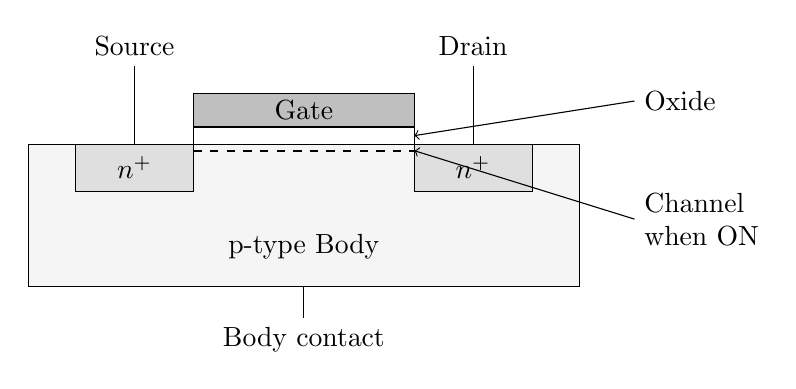
\begin{tikzpicture}[x=1cm,y=1cm]
\draw[fill=gray!8] (0,0) rectangle (7,1.8);
\draw[fill=gray!25] (0.6,1.2) rectangle (2.1,1.8);
\draw[fill=gray!25] (4.9,1.2) rectangle (6.4,1.8);
\node at (1.35,1.5) {$n^+$};\node at (5.65,1.5) {$n^+$};
\node at (3.5,0.5) {p-type Body};
\draw[fill=white] (2.1,1.8) rectangle (4.9,2.02);
\draw[fill=gray!50] (2.1,2.02) rectangle (4.9,2.45);
\node at (3.5,2.23) {Gate};
\draw (1.35,1.8)--(1.35,2.8) node[above] {Source};
\draw (5.65,1.8)--(5.65,2.8) node[above] {Drain};
\draw (3.5,0)--(3.5,-0.4) node[below] {Body contact};
\draw[<-] (4.9,1.91)--(7.7,2.35) node[right] {Oxide};
\draw[dashed,thick] (2.1,1.72)--(4.9,1.72);
\draw[<-] (4.9,1.72)--(7.7,0.85) node[right,align=left] {Channel\\when ON};
\end{tikzpicture}
\end{latin}
\caption{طرح آموزشی مقطع \lr{nMOS} بر پایه شکل \secnum{۱.۹} کتاب
\cite{weste}. خط‌چین محل تشکیل کانال را نشان می‌دهد؛ وجود همیشگی کانال را القا نمی‌کند.
خط اتصال بدنه فقط نمایش مفهومی پایانه است، نه طرح ساخت تماس.}
\label{fig:ch1-crosssection}
\end{figure}

در \lr{pMOS}، نوع ناحیه‌ها معکوس است: \lr{Source} و \lr{Drain} از نوع
\(p^+\) و بدنه از نوع \lr{n} هستند. در \lr{CMOS}، هر دو نوع روی یک تراشه
ساخته می‌شوند؛ به همین دلیل برای یکی از آن‌ها ناحیه مناسب \lr{Well} لازم است
\cite[صفحات چاپی ۷ و ۸]{weste}.
نام \lr{MOS} تاریخی است؛ جنس \lr{Gate} در دوره‌های مختلف یکسان نبوده است.

\subsection{تشکیل کانال در \lr{nMOS} و \lr{pMOS}}
برای \lr{nMOS} با بدنه و \lr{Source} نزدیک زمین، بالا بردن ولتاژ
\lr{Gate} الکترون‌ها را به سطح زیر عایق جذب می‌کند.
با ولتاژ کافی، نزدیک سطح کانالی با حامل غالب الکترون تشکیل می‌شود؛
این \lr{Inversion} مسیر هدایت میان دو ناحیه \(n^+\) را فراهم می‌کند
\cite[صفحه چاپی ۸]{weste}\cite[اسلایدهای ۶ و ۷]{mos}.
خاموش بودن یعنی مسیر کانال در مدل ساده برقرار نیست؛ این مدل جریان نشتی را حذف می‌کند.

در \lr{pMOS} با بدنه و \lr{Source} نزدیک تغذیه، پایین آوردن ولتاژ
\lr{Gate} نسبت به \lr{Source}، کانال حفره‌ای را ایجاد می‌کند.
بنابراین رفتار کنترلی آن مکمل \lr{nMOS} است.
این توصیف مقدماتی است؛ حالت‌های بار سطحی و روابط کمی در ابتدای فصل دوم استخراج می‌شوند.

\subsection{ولتاژ کنترل، آستانه و مدل \lr{Switch}}
برای \lr{nMOS} از اختلاف \(V_{gs}=V_g-V_s\) و آستانه مثبت \(V_{tn}\)
استفاده می‌کنیم. برای \lr{pMOS} در قرارداد اندازه‌های مثبت،
\(V_{sg}=V_s-V_g\) را با \(|V_{tp}|\) مقایسه می‌کنیم:
\begin{equation}\label{eq:ch1-threshold}
V_{gs}>V_{tn}\quad(\mathrm{nMOS}),\qquad
V_{sg}>|V_{tp}|\quad(\mathrm{pMOS}).
\end{equation}
در هر دو شرط، معیار اختلاف پتانسیل است، نه ولتاژ یک پایانه به‌تنهایی.
برابری با آستانه، مرز مدل ساده است؛ برای کاربرد عملی نمی‌توان آن را هدایت قوی دانست.
بدنه و آستانه نیز در مدل‌های دقیق‌تر مستقل از بایاس نیستند.

\textbf{مثال آموزشی.} در یک \lr{nMOS} فرضی با \(V_{tn}=\qty{0.3}{\volt}\)،
اگر \(V_g=\qty{1}{\volt}\) و \(V_s=\qty{0.9}{\volt}\)،
داریم \(V_{gs}=\qty{0.1}{\volt}\) و شرط روشن بودن برقرار نیست.
پس «\lr{Gate} بالا است» به‌تنهایی کافی نیست.
در گیت‌های ایستای متعارف که \lr{nMOS} خروجی را به زمین و \lr{pMOS} آن را
به تغذیه وصل می‌کند، ورودی‌های ریل‌به‌ریل این قاعده ساده را می‌دهند:
ورودی یک، \lr{nMOS} را روشن و \lr{pMOS} را خاموش می‌کند؛ ورودی صفر برعکس است
\cite[اسلاید ۲۱]{intro}. فرض می‌کنیم تغذیه از آستانه‌های لازم بیشتر است.

مدل \lr{Switch}، مسیر روشن را وصل و مسیر خاموش را قطع فرض می‌کند.
در آن، مقاومت مسیر، ظرفیت، نشتی و زمان روشن شدن را حذف می‌کنیم.
روشن بودن فقط امکان عبور جریان را نشان می‌دهد؛ بدون اختلاف ولتاژ یا بار مناسب،
جریان می‌تواند صفر باشد. شباهت تقریبی دو ناحیه \lr{Source} و \lr{Drain}
در شکل مقدماتی نیز مجوز نادیده گرفتن دیودهای بدنه یا محدودیت‌های یک قطعه واقعی نیست.

\subsection{پرسش کوتاه برای کنترل مدل}
\begin{enumerate}
\item \textbf{چرا \lr{Gate} عایق‌شده می‌تواند جریان کانال را کنترل کند؟}
کنترل با میدان الکتریکی و تغییر بار سطح انجام می‌شود؛ به عبور جریان اصلی از عایق نیاز ندارد.
\item \textbf{آیا بدون جریان رسانشی \lr{Gate}، ورودی هیچ انرژی نمی‌خواهد؟}
خیر؛ تغییر ولتاژ، ظرفیت ورودی را شارژ و دشارژ می‌کند.
\item \textbf{چرا بدنه را نباید حذف‌شده فرض کنیم؟}
پایانه چهارم بر پیوندها و آستانه اثر دارد؛ در این گام فقط اتصال متعارف و مدل ساده آن را به کار می‌بریم.
\end{enumerate}

% !TeX root = booklet-01.tex
\section{گیت‌های ایستای \lr{CMOS}}
\label{sec:book-cmos}
\label{sec:ch1-static}
\subsection{شبکه بالا و پایین چه وظیفه‌ای دارند؟}
گیت \lr{Static Complementary CMOS} یک شبکه \lr{pMOS} میان تغذیه و خروجی
به نام \lr{Pull-up Network (PUN)} و یک شبکه \lr{nMOS} میان خروجی و زمین
به نام \lr{Pull-down Network (PDN)} دارد.
برای ورودی‌های دودویی پایدار و در مدل \lr{Switch}، باید دقیقاً یکی از دو شبکه
مسیر برقرار داشته باشد \cite[بخش \secnum{۱.۴.۳}]{weste}.
این «دقیقاً یکی» هم از خروجی شناور و هم از مسیر مستقیم تغذیه به زمین جلوگیری می‌کند.

اگر شرط هدایت پایین را \(F\) بنامیم، خروجی وقتی \(F=1\) است صفر می‌شود.
پس \(Y=\overline{F}\)، و شبکه بالا باید شرط \(\overline{F}\) را پیاده کند.
\textbf{شرط هدایت شبکه پایین را نباید با تابع خروجی یکی گرفت.}
جدول \ref{tab:ch1-drive} چهار حالت کلی اتصال را نشان می‌دهد.
\begin{table}[ht]
\centering
\caption{حالت خروجی از روی هدایت دو شبکه در مدل مقدماتی؛ اثر گذرا و نشتی حذف شده است.}
\label{tab:ch1-drive}
\begin{tabular}{ccc}
\toprule
شبکه بالا & شبکه پایین & وضعیت خروجی\\
\midrule
قطع & وصل & صفر منطقی\\
وصل & قطع & یک منطقی\\
قطع & قطع & \lr{High Impedance} یا \(Z\)\\
وصل & وصل & \lr{Contention}\\
\bottomrule
\end{tabular}
\end{table}
در \(Z\)، خروجی از دو ریل جداست و مقدار آن ممکن است به بار قبلی وابسته باشد.
در \lr{Contention}، دو شبکه با هم خروجی را به دو ریل می‌کشند؛
مدل کلید ایدئال ولتاژ و جریان واقعی این اتصال را تعیین نمی‌کند.
نماد \(X\) در بحث مدار می‌تواند خروجی نامعین را نشان دهد؛
در جدول فشرده یک تابع، ممکن است به معنی «مقدار ورودی برای این سطر اهمیتی ندارد» باشد.
این دو کاربرد باید از متن تشخیص داده شوند \cite[صفحه چاپی ۱۰ و جدول بخش \secnum{۱.۴.۸}]{weste}.

\subsection{\lr{Inverter}: تحلیل اتصال، نه حفظ جدول}
در شکل \ref{fig:ch1-inverter}، ورودی \(A\) به \lr{Gate} هر دو ترانزیستور
و خروجی \(Y\) به \lr{Drain}های مشترک وصل است.
\lr{Source} بالا به \(V_{\mathrm{DD}}\) و پایین به زمین متصل است؛
بدنه‌ها نیز به‌ترتیب به تغذیه و زمین وصل‌اند و در نماد ساده رسم نشده‌اند.
\begin{figure}[ht]
\centering
\begin{latin}
\begin{circuitikz}[american]
\draw (0,2) node[pmos] (p) {} (0,-1) node[nmos] (n) {};
\draw (p.S)--(0,3.2) node[above] {$V_{\mathrm{DD}}$};
\draw (n.S)--(0,-2.2) node[ground] {};
\draw (p.D)--(0,0.5)--(n.D);
\draw (0,0.5) to[short,*-o] (1.8,0.5) node[right] {$Y$};
\draw (p.G)--(-1.6,2)--(-1.6,-1)--(n.G);
\draw (-1.6,0.5) to[short,*-o] (-2.5,0.5) node[left] {$A$};
\node[right] at (0.5,2) {pMOS};\node[right] at (0.5,-1) {nMOS};
\end{circuitikz}
\end{latin}
\caption{بازترسیم آموزشی \lr{Inverter} بر پایه شکل \secnum{۱.۱۱} کتاب و اسلاید ۲۳
\cite{weste,intro}. حباب \lr{Gate} ترانزیستور بالا نشانه \lr{pMOS} است.}
\label{fig:ch1-inverter}
\end{figure}

اگر \(A=0\)، پایین قطع و بالا وصل است؛ پس خروجی به تغذیه می‌رسد.
اگر \(A=1\)، بالا قطع و پایین وصل است؛ پس خروجی به زمین می‌رسد.
بنابراین \(Y=\overline{A}\). ورودی به خروجی اتصال رسانشی مستقیم ندارد؛
ورودی فقط وضعیت مسیرها را کنترل می‌کند.

اگر خروجی ظرفیت داشته باشد، برای رسیدن به ریل باید شارژ یا دشارژ شود.
از رابطه \(I=C\,\mathrm{d}V/\mathrm{d}t\) در بخش پیش‌نیازها می‌دانیم
این تغییر زمان می‌خواهد. مدل فعلی مقدار منطقی پایدار را می‌دهد، نه زمان گذار.
در ورودی میانی، فرض «دقیقاً یکی روشن است» لزوماً درست نیست؛
تحلیل آن به منحنی انتقال و ناحیه عملکرد جزوه سوم نیاز دارد.

\subsection{\lr{NAND}: سری در پایین، موازی در بالا}
برای دو \lr{nMOS} سری، جریان پایین فقط وقتی مسیر دارد که هر دو ورودی یک باشند؛
پس \(F_{\mathrm{PDN}}=AB\). خروجی در این حالت صفر می‌شود و تابع موردنظر
\(Y=\overline{AB}\) است. طبق \lr{De Morgan}:
\begin{equation}\label{eq:ch1-nand}
F_{\mathrm{PUN}}=\overline{AB}=\overline{A}+\overline{B}.
\end{equation}
هر \lr{pMOS} با صفر ورودی خودش روشن می‌شود، پس شبکه بالا باید دو \lr{pMOS}
موازی داشته باشد. در شکل \ref{fig:ch1-nand-nor}، مسیر هر ورودی را می‌توان دنبال کرد
\cite[بخش \secnum{۱.۴.۲}]{weste}\cite[اسلاید ۲۴]{intro}.

\begin{figure}[ht]
\centering
\begin{latin}
\begin{circuitikz}[american,scale=0.9,transform shape]
\begin{scope}
\draw (0,3) node[pmos] (pa) {} (2,3) node[pmos] (pb) {};
\draw (pa.S)--(0,4)--(2,4)--(pb.S);\node[above] at (1,4) {$V_{\mathrm{DD}}$};
\draw (pa.D)--(0,2)--(2,2)--(pb.D);
\draw (1,0.9) node[nmos] (na) {} (1,-0.8) node[nmos] (nb) {};
\draw (1,2)--(na.D) (na.S)--(nb.D) (nb.S)--(1,-1.8) node[ground] {};
\draw (2,2) to[short,*-o] (3,2) node[right] {$Y$};
\node[left] at (pa.G) {$A$};\node[left] at (pb.G) {$B$};
\node[left] at (na.G) {$A$};\node[left] at (nb.G) {$B$};
\node at (1,-2.5) {NAND};
\end{scope}
\begin{scope}[xshift=7cm]
\draw (1,3) node[pmos] (pc) {} (1,1.3) node[pmos] (pd) {};
\draw (pc.S)--(1,4) node[above] {$V_{\mathrm{DD}}$};\draw (pc.D)--(pd.S);
\draw (pd.D)--(1,0.3)--(0,0.3) (1,0.3)--(2,0.3);
\draw (0,-0.8) node[nmos] (nc) {} (2,-0.8) node[nmos] (nd) {};
\draw (0,0.3)--(nc.D) (2,0.3)--(nd.D);
\draw (nc.S)--(0,-1.8)--(2,-1.8)--(nd.S);\draw (1,-1.8) node[ground] {};
\draw (2,0.3) to[short,*-o] (3,0.3) node[right] {$Y$};
\node[left] at (pc.G) {$A$};\node[left] at (pd.G) {$B$};
\node[left] at (nc.G) {$A$};\node[left] at (nd.G) {$B$};
\node at (1,-2.5) {NOR};
\end{scope}
\end{circuitikz}
\end{latin}
\caption{بازترسیم دو گیت دوورودی بر پایه شکل‌های \secnum{۱.۱۲} و \secnum{۱.۱۶} کتاب
\cite{weste}. تکرار برچسب ورودی یعنی ولتاژ مشترک \lr{Gate}ها؛ سیم کنترل برای خوانایی حذف شده است.
بدنه همه \lr{nMOS}ها به زمین و بدنه همه \lr{pMOS}ها به تغذیه متصل است.}
\label{fig:ch1-nand-nor}
\end{figure}

برای ورودی‌های \((A,B)=(0,0)\)، هر دو \lr{pMOS} روشن‌اند و هر دو
\lr{nMOS} خاموش؛ خروجی یک می‌شود. در \((0,1)\)، مسیر پایین با ترانزیستور
کنترل‌شده با \(A\) قطع است و مسیر بالای مربوط به \(A\) وصل؛ باز خروجی یک است.
حالت \((1,0)\) مشابه است. فقط \((1,1)\) مسیر پایین را کامل و بالا را قطع می‌کند.
این چهار بررسی، جدول \ref{tab:ch1-gates} را می‌سازند.

\subsection{\lr{NOR} و تعمیم به چند ورودی}
در \lr{NOR} باید وقتی دست‌کم یک ورودی یک است، خروجی صفر شود؛
پس پایین دو \lr{nMOS} موازی با شرط \(A+B\) دارد.
بالا باید فقط وقتی هر دو ورودی صفرند هدایت کند، یعنی
\(\overline{A+B}=\overline{A}\,\overline{B}\)؛ پس دو \lr{pMOS} سری لازم است
\cite[بخش \secnum{۱.۴.۴}]{weste}\cite[اسلاید ۲۵]{intro}.
\begin{table}[ht]
\centering
\caption{خروجی پایدار دو گیت؛ هر دو برای چهار ترکیب ورودی کنترل شده‌اند.}
\label{tab:ch1-gates}
\begin{tabular}{cccc}
\toprule
\(A\)&\(B\)&\(Y_{\mathrm{NAND}}\)&\(Y_{\mathrm{NOR}}\)\\
\midrule
۰&۰&۱&۱\\
۰&۱&۱&۰\\
۱&۰&۱&۰\\
۱&۱&۰&۰\\
\bottomrule
\end{tabular}
\end{table}
برای \lr{NAND} با \(k\) ورودی، پایین \(k\) ترانزیستور سری و بالا \(k\)
ترانزیستور موازی دارد؛ برای \lr{NOR} جای سری و موازی عوض می‌شود.
تعداد کل، \(2k\) ترانزیستور است.
مثلاً \lr{NAND} سه‌ورودی \(Y=\overline{ABC}\) شش ترانزیستور دارد
\cite[اسلاید ۲۶]{intro}.
افزایش تعداد ورودی‌ها، مسیرها و ظرفیت‌ها را نیز تغییر می‌دهد؛
برابر بودن تابع منطقی مجوز نتیجه‌گیری درباره برابر بودن سرعت نیست.

\subsection{گیت \lr{Compound} و اصل \lr{Conduction Complements}}
برای ساخت گیت \(Y=\overline{AB+CD}\)، نخست عبارت داخل مکمل را
شرط هدایت پایین می‌گیریم:
\begin{equation}\label{eq:ch1-aoi}
F_{\mathrm{PDN}}=AB+CD,\qquad
F_{\mathrm{PUN}}=(\overline{A}+\overline{B})(\overline{C}+\overline{D}).
\end{equation}
پایین دو شاخه موازی دارد که هر شاخه شامل دو \lr{nMOS} سری است.
بالا، گروه موازی \(A,B\) از نوع \lr{pMOS} را با گروه موازی \(C,D\) سری می‌کنیم.
عملگرها تغییر کرده‌اند، ولی برچسب \lr{Gate} هر ترانزیستور همان ورودی اصلی است؛
برای هر \lr{pMOS}، مکمل بودن شرط هدایت از خود نوع ترانزیستور می‌آید.
این تبدیل سری به موازی و برعکس، \lr{Conduction Complements} نام دارد
\cite[بخش \secnum{۱.۴.۵} و شکل \secnum{۱.۱۸}]{weste}.

شکل \ref{fig:ch1-aoi} شبکه‌ها را بدون شلوغی نماد ترانزیستور نشان می‌دهد.
هر بلوک یک ترانزیستور با نوع و نام ورودی کنترل است؛ نقطه‌ها اتصال الکتریکی‌اند.
\begin{figure}[ht]
\centering
\begin{latin}
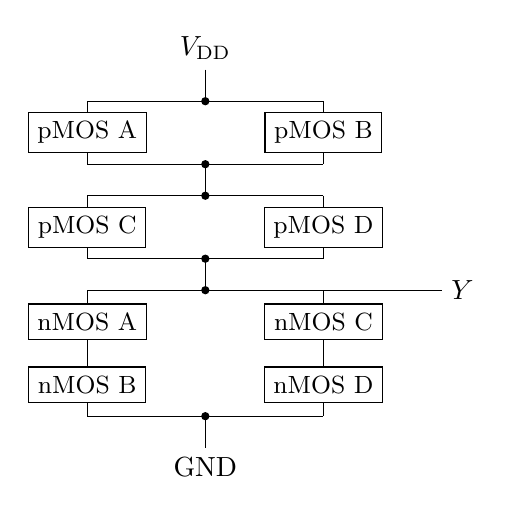
\begin{tikzpicture}[x=1cm,y=0.8cm]
\node[above] at (0,6) {$V_{\mathrm{DD}}$};
\draw (0,6)--(0,5.5)--(-1.5,5.5) (0,5.5)--(1.5,5.5);
\draw (-1.5,5.5)--(-1.5,4.5) node[midway,draw,fill=white,font=\small] {pMOS A};
\draw (1.5,5.5)--(1.5,4.5) node[midway,draw,fill=white,font=\small] {pMOS B};
\draw (-1.5,4.5)--(1.5,4.5);\draw (0,4.5)--(0,4)--(-1.5,4) (0,4)--(1.5,4);
\draw (-1.5,4)--(-1.5,3) node[midway,draw,fill=white,font=\small] {pMOS C};
\draw (1.5,4)--(1.5,3) node[midway,draw,fill=white,font=\small] {pMOS D};
\draw (-1.5,3)--(1.5,3);\draw (0,3)--(0,2.5)--(3,2.5) node[right] {$Y$};
\draw (0,2.5)--(-1.5,2.5)--(-1.5,1.5) node[midway,draw,fill=white,font=\small] {nMOS A};
\draw (0,2.5)--(1.5,2.5)--(1.5,1.5) node[midway,draw,fill=white,font=\small] {nMOS C};
\draw (-1.5,1.5)--(-1.5,0.5) node[midway,draw,fill=white,font=\small] {nMOS B};
\draw (1.5,1.5)--(1.5,0.5) node[midway,draw,fill=white,font=\small] {nMOS D};
\draw (-1.5,0.5)--(1.5,0.5);\draw (0,0.5)--(0,0) node[below] {GND};
\foreach \x/\y in {0/5.5,0/4.5,0/4,0/3,0/2.5,0/0.5} {\fill (\x,\y) circle (1.5pt);}
\end{tikzpicture}
\end{latin}
\caption{نمای توپولوژی آموزشی \lr{AOI22} برای رابطه \eqref{eq:ch1-aoi}.
بلوک‌های برچسب‌دار در این نمایش جایگزین نماد ترانزیستورند؛
وضعیت هدایت هر بلوک به نوع ترانزیستور و ورودی نوشته‌شده در آن بستگی دارد.}
\label{fig:ch1-aoi}
\end{figure}

نام \lr{AND-OR-Invert (AOI22)} می‌گوید دو گروه \lr{AND} دوورودی داریم،
خروجی آن‌ها \lr{OR} و سپس معکوس می‌شود.
در مثال \((A,B,C,D)=(1,1,0,0)\)، شاخه \(AB\) پایین وصل است؛
در بالا گروه \(A,B\) کاملاً قطع است، پس \(Y=0\).
در \((1,0,1,0)\)، هر شاخه پایین یک ترانزیستور قطع دارد؛
در بالا از \(B\) و \(D\) مسیر کامل داریم، پس \(Y=1\).
این دو مثال جای بررسی تمام حالت‌ها را نمی‌گیرند؛ رابطه مکمل، پوشش همه حالت‌ها را می‌دهد.

\textbf{مثال کتاب، \lr{OAI31}.} برای
\(Y=\overline{(A+B+C)D}\)، پایین گروه موازی \(A,B,C\) را با \(D\) سری می‌کنیم.
بالا گروه سری سه \lr{pMOS} با کنترل \(A,B,C\) را با یک \lr{pMOS} کنترل‌شده با \(D\)
موازی می‌کنیم؛ چون شرط بالا
\(\overline{A}\,\overline{B}\,\overline{C}+\overline{D}\) است.
این هشت ترانزیستور، تابع مثال \secnum{۱.۲} کتاب را می‌سازند
\cite[صفحه چاپی ۱۲]{weste}.

\subsection{چرا \lr{AND} را با یک \lr{NAND} و یک \lr{Inverter} می‌سازیم؟}
در خانواده محدود شبکه‌های مکمل ایستا که ورودی‌های غیرمعکوس مستقیماً
\lr{Gate}ها را کنترل می‌کنند، روشن شدن مسیر پایین خروجی را صفر می‌کند؛
ازاین‌رو گیت یک‌مرحله‌ای، تابع معکوس‌کننده ورودی‌هاست.
جابه‌جا کردن ساده \lr{nMOS} و \lr{pMOS} برای ساخت \lr{Buffer} مناسب نیست؛
با انتقال سطوح ضعیف روبه‌رو می‌شویم \cite[صفحه چاپی ۱۴]{weste}.
به‌جای آن، دو معکوس‌سازی می‌دهند
\[
 Y=\overline{\overline{AB}}=AB.
\]
برای \lr{OR} نیز \lr{NOR} و سپس \lr{Inverter} به کار می‌رود.

\lr{AND} دوورودی با این روش شش ترانزیستور دارد: چهار برای \lr{NAND}
و دو برای \lr{Inverter}. ساخت تابع \lr{AOI22} از دو \lr{AND}، یک \lr{OR}
و یک \lr{Inverter} با این سلول‌های ساده، \(6+6+6+2=20\)
ترانزیستور می‌خواهد؛ گیت \lr{Compound} فقط هشت ترانزیستور دارد.
این مقایسه شمارش قطعات است؛ برای نتیجه قطعی درباره \lr{Delay} یا توان باید
اندازه ترانزیستورها، بار و مسیرها نیز تحلیل شوند \cite[شکل \secnum{۱.۲۴}]{weste}.

\subsection{کنترل اعتبار گیت ایستا}
برای هر ترکیب ورودی، ابتدا قطع یا وصل بودن تک‌تک قطعات و سپس وجود مسیر کامل
را مشخص می‌کنیم. اگر پایین هدایت دارد، بالا باید قطع باشد و برعکس.
این کنترل برای تمام ورودی‌ها، شرط منطقی طراحی است.
در مدل ایدئال پایدار، ابعاد ترانزیستورها جدول درستی را عوض نمی‌کنند؛
در مدار واقعی، ابعاد بر زمان و توان و رفتار گذرا اثر دارند.
عبارت «توان ساکن صفر» نیز فقط به مدل بدون نشتی و ورودی‌های پایدار معتبر تعلق دارد؛
بار خازنی و هدایت هم‌زمان در گذار، همچنان انرژی مصرف می‌کنند.

\BookletSubsections{notes/booklet-01/ch1-pass-mux}
\BookletSubsections{notes/booklet-01/ch1-storage}
\section{ساخت و \lr{Layout} مدارهای \lr{CMOS}}
\label{sec:book-fabrication}
این بخش، زیربخش‌های \secnum{۱.۵.۱} تا \secnum{۱.۵.۵} کتاب را پوشش می‌دهد.
فرآیند \lr{n-well CMOS} و قواعد هندسی، مدل آموزشی مرجع هستند.
\BookletSubsections{notes/booklet-01/ch1-fabrication}
\BookletSubsections{notes/booklet-01/ch1-layout-rules}
\BookletSubsections{notes/booklet-01/ch1-layout-examples}
% !TeX root = booklet-01.tex
\section{تقسیم طراحی و سطوح \lr{Abstraction}}
\label{sec:book-partitioning}
\subsection{چرا طراحی بزرگ را تقسیم می‌کنیم؟}
خواندن یک \lr{Inverter} با دنبال کردن دو ترانزیستور ممکن بود؛
در یک پردازنده، بررسی هم‌زمان تمام ترانزیستورها روش مناسبی برای فهم عملکرد نیست.
\lr{Abstraction} یعنی جزئیات نامربوط به پرسش فعلی را موقتاً پنهان کنیم،
ولی قرارداد ورودی، خروجی و رفتار را نگه داریم.
\lr{Design Partitioning} نیز تقسیم سیستم به بخش‌هایی با مسئولیت و رابط مشخص است
\cite[بخش \secnum{۱.۶}]{weste}.

تقسیم بیش‌ازحد مستقل، ممکن است هر بلوک را بهینه ولی ترکیب کل را نامناسب کند؛
وابستگی همه بلوک‌ها به همه جزئیات یکدیگر نیز پیشرفت را کند می‌کند.
برای مثال، کوچک کردن یک بلوک با خروجی ضعیف می‌تواند نیاز به بافر و تاخیر بلوک بعدی را بیشتر کند.
پس بهینه‌سازی باید اثر بر همسایه‌ها و هدف کل سیستم را نیز بسنجد.

\subsection{پنج سطح طراحی را با یک مثال تشخیص دهیم}
جدول \ref{tab:design-levels} پنج سطح بخش \secnum{۱.۶.۱} کتاب را روی مثال
جمع دو داده نشان می‌دهد \cite{weste}\cite[اسلاید ۱۷]{intro}.
ستون پرسش، دلیل متفاوت بودن سطح‌ها را مشخص می‌کند.
\begin{table}[ht]
\centering
\caption{سطوح طراحی و نمونه تصمیم در هر سطح}
\label{tab:design-levels}
\begin{tabularx}{\textwidth}{l>{\raggedleft\arraybackslash}X>{\raggedleft\arraybackslash}X}
\toprule
سطح & پرسش اصلی & نمونه تصمیم\\
\midrule
\lr{Architecture}&کار قابل مشاهده سیستم چیست؟&دستور جمع، ثبات‌های قابل مشاهده و معنای نتیجه\\
\lr{Microarchitecture}&عملیات با چه منابعی و در چه چرخه‌هایی انجام می‌شود؟&یک \lr{ALU} مشترک یا چند واحد؛ محل ثبات‌های میانی\\
\lr{Logic}&واحدها از چه منطق و حالت‌هایی ساخته می‌شوند؟&جمع‌کننده \lr{Ripple Carry} یا \lr{Carry Lookahead}\\
\lr{Circuit}&منطق با چه مدار ترانزیستوری پیاده می‌شود؟&گیت‌های \lr{Static CMOS} یا مدار عبوری\\
\lr{Physical}&اجزا و اتصال‌ها کجا و با چه هندسه‌ای قرار می‌گیرند؟&جانمایی سلول و مسیر فلزی\\
\bottomrule
\end{tabularx}
\end{table}

دو پیاده‌سازی می‌توانند دستورهای یکسانی اجرا کنند ولی تعداد چرخه، مصرف توان
و مساحت متفاوت داشته باشند. بنابراین \lr{Architecture} با
\lr{Microarchitecture} یکی نیست. همچنین انتخاب الگوریتم جمع‌کننده با انتخاب
مدار ترانزیستوری گیت آن یک تصمیم نیست.
\lr{ALU} مخفف \lr{Arithmetic/Logic Unit} است و عملیات حسابی و منطقی را انجام می‌دهد.

این سطح‌ها دیوار مستقل نیستند. اگر یک مسیر فیزیکی طولانی شود، ممکن است
هدف فرکانس برآورده نشود و تعداد مرحله‌های زمانی یا ساختار منطقی تغییر کند.
کتاب بر تعامل طراحی \lr{Microarchitecture}، منطق، مدار و شکل فیزیکی تاکید می‌کند؛
ترتیب توضیح آموزشی، تضمین یک فرایند یک‌طرفه و بدون بازگشت نیست.

\subsection{چهار اصل \lr{Structured Design}}
\begin{enumerate}
\item \textbf{\lr{Hierarchy}:} سیستم به بلوک، زیر‌بلوک و سلول تقسیم می‌شود.
برای مثال پردازنده شامل \lr{Datapath} و کنترل است؛ جمع‌کننده داخل \lr{Datapath}
نیز از \lr{Full Adder}ها ساخته می‌شود.
\item \textbf{\lr{Regularity}:} تعداد نوع‌های متفاوت بلوک کم و استفاده مجدد زیاد باشد.
هشت نمونه یک \lr{MUX} تک‌بیتی، منطق انتخاب هشت‌بیتی را می‌سازند؛
لازم نیست هر بیت از ابتدا با سبک متفاوت طراحی شود.
\item \textbf{\lr{Modularity}:} رابط بلوک روشن باشد؛ عرض داده، قطبیت کنترل،
زمان معتبر بودن و بار قابل راه‌اندازی جزو قراردادند.
نام برابر دو سیگنال یا اتصال سیم به‌تنهایی، سازگاری رابط را اثبات نمی‌کند.
\item \textbf{\lr{Locality}:} اطلاعات در زمان و مکان نزدیک استفاده‌اش نگه داشته شود.
قرار دادن ثبات موقت نزدیک واحد محاسبه می‌تواند نیاز به رفت‌وآمد داده را کمتر کند؛
نتیجه کمی آن به سیم‌کشی و مدل مدار وابسته است.
\end{enumerate}
این اصول از بخش \secnum{۱.۶.۲} کتاب و اسلاید ۱۶ گرفته شده‌اند
\cite{weste,intro}. تکرار یک سلول بررسی‌شده، تعداد مسئله‌های مستقل را کم می‌کند؛
اما اتصال و زمان‌بندی نمونه‌های کنار هم هنوز باید کنترل شوند.

\subsection{سه دامنه \lr{Behavioral}، \lr{Structural} و \lr{Physical}}
سطح \lr{Abstraction} میزان جزئیات را می‌گوید؛ دامنه، نوع توصیف را.
در نمودار \lr{Y}، سه دامنه در چند سطح جزئیات وجود دارند
\cite[بخش \secnum{۱.۶.۳} و شکل \secnum{۱.۴۸}]{weste}:
\lr{Behavioral} می‌گوید «چه می‌کند»، \lr{Structural} می‌گوید «از چه اجزایی و اتصال‌هایی ساخته شده»
و \lr{Physical} هندسه و جای اجزا را توصیف می‌کند.

برای یک \lr{Full Adder}، رابطه جمع و نقلی توصیف رفتاری است؛
شبکه \lr{XOR} و گیت‌های نقلی توصیف ساختاری است؛
مستطیل‌های لایه‌ها و تماس‌ها توصیف فیزیکی‌اند.
پس \lr{Behavioral} فقط مخصوص سطح پردازنده و \lr{Physical} فقط مخصوص یک ترانزیستور نیست؛
یک تراشه نیز \lr{Floorplan} فیزیکی دارد.

در شکل \ref{fig:design-domains}، خط‌های بین دامنه‌ها تبدیل توصیف را نشان می‌دهند.
پس از هر تبدیل باید معادل بودن رفتار موردنظر بررسی شود؛
هندسه کوچک یا خروجی ابزار خودکار به‌خودی‌خود حفظ عملکرد را ثابت نمی‌کند.
\begin{figure}[ht]
\centering
\begin{latin}
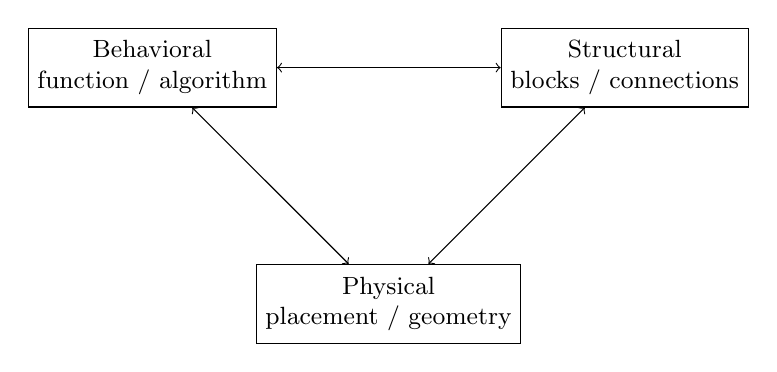
\begin{tikzpicture}[font=\small]
\node[draw,align=center,minimum width=3.1cm,minimum height=1cm] (b) at (-3,1.6) {Behavioral\\function / algorithm};
\node[draw,align=center,minimum width=3.1cm,minimum height=1cm] (s) at (3,1.6) {Structural\\blocks / connections};
\node[draw,align=center,minimum width=3.1cm,minimum height=1cm] (p) at (0,-1.4) {Physical\\placement / geometry};
\draw[<->] (b)--(s);\draw[<->] (b)--(p);\draw[<->] (s)--(p);
\end{tikzpicture}
\end{latin}
\caption{بازنمایی مفهومی رابطه سه دامنه، بر پایه بحث نمودار \lr{Y} کتاب
\cite{weste}. این شکل بازتولید هندسی خود نمودار \lr{Y} نیست؛
تبدیل دامنه‌ها در یک سطح مشخص را برجسته می‌کند.}
\label{fig:design-domains}
\end{figure}

\subsection{مثال بررسی رابط}
فرض کنید بلوکی \lr{MUX} هشت‌بیتی دارد و انتخابش با یک بیت \(S\) انجام می‌شود.
باید معلوم باشد \(S=0\) کدام ورودی را انتخاب می‌کند، هر ورودی چه زمانی معتبر است
و خروجی چه زمانی مصرف می‌شود. اتصال ورودی هفت‌بیتی به آن، یا برداشت معکوس از
معنای \(S\)، می‌تواند عملکرد را عوض کند؛ حتی اگر نام بلوک درست باشد.
در ادامه، همین انضباط را برای رابط پردازنده و حافظه به کار می‌بریم.

\section{مثال پردازنده آموزشی \lr{MIPS}}
\label{sec:book-mips}
در زیرمجموعه آموزشی کتاب، داده و \lr{PC} هشت‌بیتی و دستور ۳۲ بیتی است.
هر جا قرارداد با معماری کامل متفاوت باشد، فرض مثال در متن مشخص می‌شود.
\BookletSubsections{notes/booklet-01/ch1-mips-architecture}
\BookletSubsections{notes/booklet-01/ch1-mips-microarchitecture}
\section{از رابط بلوک‌ها تا \lr{Logic Design} و \lr{HDL}}
\label{sec:book-logic-design}
\BookletSubsections{notes/booklet-01/ch1-logic-hdl}
\section{طراحی در سطح مدار}
\label{sec:book-circuit-design}
\subsection{جریان و خازن چگونه تأخیر را تعیین می‌کنند؟}
در \lr{Circuit Design}، برای تابع منطقی مشخص، شبکه ترانزیستورها و اندازه آن‌ها
انتخاب می‌شود. خروجی یک گیت، ورودی گیت بعدی و سیم میان آن‌ها را راه‌اندازی می‌کند.
عایق \lr{Gate} موجب رفتار خازنی ورودی است. خازن‌های \lr{Diffusion} و سیم نیز به بار
خروجی افزوده می‌شوند. بنابراین صفر و یک‌شدن خروجی به جابه‌جایی بار الکتریکی نیاز دارد
\cite[بخش \secnum{۱.۹}، شکل \secnum{۱.۶۰}]{weste}.

اگر خازن معادل بار را \(C_L\) بنامیم، در مدل خازن ثابت رابطه بار و ولتاژ
\(Q=C_LV\) است. با تغییر ولتاژ به اندازه \(\Delta V\)، بار به اندازه
\(\Delta Q=C_L\Delta V\) تغییر می‌کند. جریان متوسط، بار جابه‌جاشده تقسیم بر زمان است.
از این دو تعریف، بدون نیاز به حل معادله دیفرانسیل، داریم
\begin{equation}
 I_{\mathrm{avg}}=\frac{\Delta Q}{\Delta t}
 \quad\Longrightarrow\quad
 \Delta t=\frac{C_L\Delta V}{I_{\mathrm{avg}}}.
 \label{eq:impl-charge-delay}
\end{equation}
برای جریان لحظه‌ای همین معنا به صورت \(i=C_L\,dV/dt\) نوشته می‌شود.
نماد \(dV/dt\) سرعت تغییر ولتاژ را بیان می‌کند. برای تخمین زمان تغییر کامل ولتاژ
از صفر تا \(V_{DD}\)، کتاب از تقریب
\begin{equation}
 t_{\mathrm{sw}}\approx\frac{C_LV_{DD}}{I_{\mathrm{avg}}}
 \label{eq:impl-full-swing}
\end{equation}
استفاده می‌کند. جریان ترانزیستور در طول گذار تغییر می‌کند، بنابراین انتخاب
\(I_{\mathrm{avg}}\) باید با همان بازه ولتاژ سازگار باشد. \lr{Propagation Delay}
معمولاً میان نقاط مرجع گذار ورودی و خروجی، مانند نصف ولتاژ تغذیه، اندازه‌گیری می‌شود.
رابطه \eqref{eq:impl-full-swing} یک تخمین مرتبه اول برای زمان تغییر ولتاژ است.

کنترل واحدها نتیجه را روشن می‌کند. چون \(\unit{\farad}=\unit{\coulomb\per\volt}\)
و \(\unit{\ampere}=\unit{\coulomb\per\second}\)، واحد
\(C_LV/I\) برابر ثانیه می‌شود. بار بیشتر، زمان بیشتر می‌خواهد. جریان قوی‌تر همان بار
را سریع‌تر جابه‌جا می‌کند. در مدل ایدئال، اگر \(C_L=0\) باشد این سهم از تأخیر صفر
می‌شود. اگر جریان به صفر نزدیک شود، زمان لازم افزایش می‌یابد.

در مثال فرضی، \(C_L=\qty{20}{\femto\farad}\)، \(V_{DD}=\qty{1}{\volt}\)
و \(I_{\mathrm{avg}}=\qty{100}{\micro\ampere}\) هستند. جای‌گذاری مرحله‌ای می‌دهد
\begin{equation*}
 t_{\mathrm{sw}}\approx
 \frac{20\times10^{-15}\times1}{100\times10^{-6}}\,\unit{\second}
 =2\times10^{-10}\,\unit{\second}=\qty{200}{\pico\second}.
\end{equation*}
دوبرابرشدن بار با جریان ثابت، زمان را به \qty{400}{\pico\second} می‌رساند.
این اعداد صرفاً برای تمرین تبدیل پیشوند و تحلیل رابطه انتخاب شده‌اند.

\subsection{اثر عرض ترانزیستور و بار مرحله بعد}
با ثابت‌بودن طول و شرایط بایاس، مدل مقدماتی جریان و خازن ورودی را متناسب با عرض
\(W\) می‌گیرد \cite[صفحه ۴۲]{weste}. افزایش عرض، جریان راه‌انداز و هم‌زمان بار
دیده‌شده در مرحله قبل را افزایش می‌دهد. اگر ضریب بزرگ‌کردن ترانزیستور \(s>0\)
باشد، برای تحلیل ساده می‌توان نوشت
\begin{equation}
 I(s)\approx sI_0,\qquad
 C_L(s)\approx C_{\mathrm{ext}}+sC_{\mathrm{int},0},\qquad
 t(s)\approx\frac{V_{DD}}{I_0}
 \left(\frac{C_{\mathrm{ext}}}{s}+C_{\mathrm{int},0}\right).
 \label{eq:impl-sizing}
\end{equation}
در این مدل، \(C_{\mathrm{ext}}\) بار ثابت خارجی و \(C_{\mathrm{int},0}\) سهم داخلی
در اندازه اولیه است. بزرگ‌کردن گیت، سهم بار ثابت را سریع‌تر راه‌اندازی می‌کند، اما
سهم خازن داخلی نیز رشد می‌کند. خازن ورودی بزرگ‌تر، تأخیر و انرژی مرحله قبل را تغییر
می‌دهد. انتخاب اندازه به مسیر چندمرحله‌ای، \lr{Fan-in}، \lr{Fan-out}، سیم و محدودیت
مساحت وابسته است. مدل‌های دقیق‌تر جریان و خازن در فصل ۲ و روش‌های اندازه‌گذاری در فصل ۴ آمده‌اند.

\subsection{استخراج انرژی و توان از شارژ خازن}
توان لحظه‌ای منبع تغذیه برابر \(p=V_{DD}i\) است. برای شارژ کامل یک خازن از صفر
تا \(V_{DD}\)، منبع بار \(Q=C_LV_{DD}\) تحویل می‌دهد. چون ولتاژ منبع ثابت است،
انرژی دریافت‌شده از منبع برابر می‌شود با
\begin{equation}
 E_{\mathrm{supply}}=V_{DD}Q=C_LV_{DD}^2.
 \label{eq:impl-supply-energy}
\end{equation}
انرژی ذخیره‌شده در خود خازن از جمع انرژی‌های کوچک \(V\,dQ\) به دست می‌آید.
با \(dQ=C_L\,dV\)، مساحت زیر خط \(C_LV\) از صفر تا \(V_{DD}\) یک مثلث است، پس
\begin{equation}
 E_C=\int_0^{V_{DD}}C_LV\,dV=\frac12 C_LV_{DD}^2.
 \label{eq:impl-stored-energy}
\end{equation}
در شارژ معمول مقاومتی، نیم دیگر انرژی منبع در مسیر شارژ تلف می‌شود. هنگام تخلیه،
انرژی ذخیره‌شده نیز در مسیر تخلیه تلف می‌شود. بنابراین انرژی یک چرخه کامل
\(0\rightarrow1\rightarrow0\) در این مدل برابر \(C_LV_{DD}^2\) است.

اگر در هر ثانیه \(f_{\mathrm{cyc}}\) چرخه کامل رخ دهد، توان متوسط برابر انرژی
هر چرخه ضرب‌در تعداد چرخه در ثانیه خواهد بود
\begin{equation}
 P_{\mathrm{dyn}}=C_LV_{DD}^2f_{\mathrm{cyc}}.
 \label{eq:impl-dynamic-power}
\end{equation}
این همان صورت رابطه کتاب است \cite[صفحه ۴۳]{weste}. برای ارتباط با \lr{Clock}،
\(\alpha_{01}\) را متوسط تعداد گذارهای \(0\rightarrow1\) در هر دوره \lr{Clock}
تعریف می‌کنیم. در حالت پایدار، فرکانس شارژ \(\alpha_{01}f_{\mathrm{clk}}\) است، پس
\begin{equation}
 P_{\mathrm{dyn}}=\alpha_{01}C_LV_{DD}^2f_{\mathrm{clk}}.
 \label{eq:impl-activity-power}
\end{equation}
با شمارش مجموع گذارهای صعودی و نزولی، باید تعریف ضریب فعالیت را نیز عوض کرد.
برای سیگنال متناوب \(0,1,0,1,\ldots\) در نمونه‌های متوالی \lr{Clock}، در هر دو
دوره یک شارژ رخ می‌دهد، بنابراین \(\alpha_{01}=1/2\) است. برای چند گره، سهم
\(\alpha_{01,k}C_kV_{DD}^2f_{\mathrm{clk}}\) هر گره جمع می‌شود.

در مثال فرضی \(C_L=\qty{20}{\femto\farad}\)، \(V_{DD}=\qty{1}{\volt}\)،
\(f_{\mathrm{clk}}=\qty{100}{\mega\hertz}\) و \(\alpha_{01}=0.25\)، داریم
\begin{equation}
 P_{\mathrm{dyn}}=0.25(20\times10^{-15})(1)^2(100\times10^6)
 \,\unit{\watt}=\qty{0.50}{\micro\watt}.
 \label{eq:impl-power-example}
\end{equation}
کاهش ولتاژ به \qty{0.8}{\volt} با ثابت‌فرض‌کردن سایر عوامل، توان را در
\(0.8^2=0.64\) ضرب می‌کند و به \qty{0.32}{\micro\watt} می‌رساند. جریان ترانزیستور
نیز به ولتاژ وابسته است، پس بررسی سرعت به مدل جریان نیاز دارد.

\subsection{توان \lr{Static} و انتخاب پیاده‌سازی}
ترانزیستور خاموش واقعی جریان نشتی دارد. اگر جریان متوسط مستقیم از تغذیه به زمین
را \(I_{\mathrm{static}}\) بنامیم، از تعریف توان به دست می‌آید
\begin{equation}
 P_{\mathrm{static}}=V_{DD}I_{\mathrm{static}}.
 \label{eq:impl-static-power}
\end{equation}
این رابطه حتی در نبود تغییر منطقی خروجی کاربرد دارد \cite[صفحه ۴۳]{weste}.
برای جریان فرضی \qty{10}{\nano\ampere} و تغذیه \qty{1}{\volt}، توان
\qty{10}{\nano\watt} است. مجموع این سهم و مثال \eqref{eq:impl-power-example}،
در مدل دو مؤلفه‌ای، \qty{0.51}{\micro\watt} می‌شود. جریان گذرای هم‌پوشانی روشن‌شدن
شبکه‌های \lr{Pull-up} و \lr{Pull-down} نیز می‌تواند سهم دیگری ایجاد کند که در تحلیل
تفصیلی فصل توان بررسی می‌شود.

\lr{Synthesis} با انتخاب گیت‌های کتابخانه و اندازه آن‌ها، تابع منطقی را تحت
محدودیت‌های طراحی پیاده می‌کند. \lr{Custom Circuit Design} امکان انتخاب شبکه
ترانزیستوری متناسب با تابع را فراهم می‌سازد. کتاب اهمیت آن را برای بخش‌های دارای
نیاز سرعت یا توان ویژه و برای حجم تولید توجیه‌کننده هزینه مهندسی توضیح می‌دهد.
\lr{Area}، توان، سرعت و تلاش طراحی باید هم‌زمان سنجیده شوند.

\subsection{مثال \lr{Carry} با ۲۶ و ۱۲ ترانزیستور}
در \lr{Full Adder}، ورودی‌های تک‌بیتی \(a,b,c\) هستند و \(c\) نقش \lr{Carry-in}
را دارد. خروجی \(c_{\mathrm{out}}\) وقتی یک می‌شود که دست‌کم دو ورودی یک باشند.
تابع آن برابر است با
\begin{equation}
 c_{\mathrm{out}}=ab+ac+bc.
 \label{eq:impl-carry-majority}
\end{equation}
در این معادله، کنارهم‌نوشتن نمادها به معنای \lr{AND} و علامت جمع به معنای
\lr{OR} است. برای مثال \(a=b=1\) با هر مقدار \(c\)، خروجی یک می‌دهد.
اگر فقط یک ورودی یک باشد، هر سه حاصل‌ضرب صفر می‌شوند.

پیاده‌سازی شکل \secnum{۱.۶۱} کتاب از سه \lr{AND2} و یک \lr{OR3} تشکیل می‌شود
\cite{weste}. \lr{AND2} در \lr{Static CMOS} معمول، یک \lr{NAND2} چهارترانزیستوری
و یک \lr{Inverter} دوترانزیستوری دارد. \lr{OR3} نیز از \lr{NOR3} شش‌ترانزیستوری
و یک \lr{Inverter} ساخته می‌شود. بنابراین
\begin{equation*}
 N_{\mathrm{gate}}=3(4+2)+(6+2)=26.
\end{equation*}
مسیر ورودی تا خروجی از چهار مرحله وارون‌کننده منطقی عبور می‌کند.
تأخیر هر مرحله تابع اندازه و بار آن است.

برای ساخت مدار فشرده، ابتدا تابع را عامل‌گیری می‌کنیم
\begin{equation}
 F=ab+c(a+b),\qquad c_n=\overline F,\qquad c_{\mathrm{out}}=\overline{c_n}.
 \label{eq:impl-factored-carry}
\end{equation}
شبکه \lr{Pull-down} گره \(c_n\)، یک شاخه دوترانزیستوری سری با کنترل \(a,b\)
و یک شاخه شامل \(c\) در سری با دو ترانزیستور موازی \(a,b\) دارد. این شبکه پنج
\lr{nMOS} می‌خواهد. هرگاه \(F=1\) باشد، مسیری تا زمین برقرار می‌شود.

شبکه \lr{Pull-up} شکل کتاب نیز پنج \lr{pMOS} دارد. شرط هدایت آن را با
\(\bar a,\bar b,\bar c\) بیان می‌کنیم، زیرا \lr{pMOS} با ورودی صفر روشن می‌شود.
با قانون \lr{De Morgan} و توزیع حاصل‌ضرب داریم
\begin{align*}
 \overline F
 &=(\bar a+\bar b)(\bar c+\bar a\bar b)\\
 &=\bar c(\bar a+\bar b)+\bar a\bar b.
\end{align*}
جمله اول، \(c\) در سری با موازی \(a,b\)، و جمله دوم، سری \(a,b\) در شبکه
\lr{pMOS} را مشخص می‌کند. بنابراین برای هر ورودی دودویی پایدار، یکی از شبکه‌ها
گره \(c_n\) را به تغذیه مناسب می‌رساند. \lr{Inverter} پایانی دو ترانزیستور دیگر دارد
و تعداد کل \(5+5+2=12\) می‌شود. مسیر منطقی شامل یک گیت مرکب و یک
\lr{Inverter} است. مقایسه سرعت عددی، به اندازه ترانزیستورها و بارها نیاز دارد.

جدول \ref{tab:impl-carry} همه حالت‌های دودویی را کنترل می‌کند. ستون \lr{PDN}
و \lr{PUN}، وجود مسیر رسانا برای گره \(c_n\) را نشان می‌دهند.
\begin{table}[ht]
\centering
\caption{کنترل کامل تابع و شبکه‌های \lr{Carry} در مدل سوئیچی ایدئال.}
\label{tab:impl-carry}
\begin{tabular}{ccccccc}
\toprule
\(a\)&\(b\)&\(c\)&\lr{PDN}&\lr{PUN}&\(c_n\)&\(c_{\mathrm{out}}\)\\
\midrule
۰&۰&۰&۰&۱&۱&۰\\
۰&۰&۱&۰&۱&۱&۰\\
۰&۱&۰&۰&۱&۱&۰\\
۰&۱&۱&۱&۰&۰&۱\\
۱&۰&۰&۰&۱&۱&۰\\
۱&۰&۱&۱&۰&۰&۱\\
۱&۱&۰&۱&۰&۰&۱\\
۱&۱&۱&۱&۰&۰&۱\\
\bottomrule
\end{tabular}
\end{table}

\subsection{\lr{Schematic} و دو سطح \lr{Netlist}}
\lr{Schematic} اتصال‌ها را به صورت تصویر و \lr{Netlist} همان ارتباط‌ها را به صورت
متن نمایش می‌دهد. در توصیف ساختاری گیت‌ها، نمونه آموزشی تابع \lr{Carry} چنین است
\cite[صفحات ۴۳ و ۴۴]{weste}.
\begin{latin}
\small
\begin{verbatim}
module carry(input logic a, b, c, output logic cout);
  logic x, y, z;
  and g1(x, a, b);
  and g2(y, a, c);
  and g3(z, b, c);
  or  g4(cout, x, y, z);
endmodule
\end{verbatim}
\end{latin}
در این \lr{Verilog}، نخستین آرگومان هر گیت خروجی است. نام‌های \code{g1} تا
\code{g4} شناسه نمونه‌ها و \code{x}، \code{y} و \code{z} سیم‌های میانی هستند.
گیت عمومی هنوز اندازه، خازن و مدل فناوری را مشخص نمی‌کند.

در توصیف سوئیچی کتاب، \code{tranif1} با کنترل یک و \code{tranif0} با کنترل صفر
اتصال برقرار می‌کنند. ترتیب آرگومان آن‌ها دو پایانه مسیر و سپس کنترل است.
برای نمونه \code{tranif1 n3(cn, i1, c)} گره‌های \code{cn} و \code{i1} را هنگام
یک‌بودن \code{c} وصل می‌کند. مسیر در این مدل دوطرفه است. \code{supply0} و
\code{supply1} به‌ترتیب زمین و تغذیه منطقی، و \code{tri} گره سیمی با قابلیت حالت
پرامپدانس را معرفی می‌کنند. این نمایش برای بررسی اتصال و عملکرد سوئیچی مناسب است.

برای تحلیل پیوسته ولتاژ، جریان، تأخیر و توان، \lr{SPICE} به مدل افزاره و ابعاد نیاز
دارد. ترانزیستور \lr{MOS} چهار پایانه \lr{Drain}، \lr{Gate}، \lr{Source} و
\lr{Body} دارد. خط معرفی آن در کتاب به ترتیب زیر است
\cite[صفحات ۴۴ و ۴۵]{weste}.
\begin{latin}
\small
\begin{verbatim}
Mname drain gate source body model W=width L=length
+ AD=drain_area AS=source_area
Cname node1 node2 value
\end{verbatim}
\end{latin}
علامت \code{+} در آغاز خط، ادامه همان دستور را نشان می‌دهد. \code{W} و
\code{L} عرض و طول کانال، و \code{AD} و \code{AS} مساحت‌های اتصال
\lr{Drain} و \lr{Source} هستند. نام مدل، پارامترهای فناوری را به نمونه مرتبط می‌کند.
این ترتیب با ترتیب آرگومان گیت‌های \lr{Verilog} تفاوت دارد.

فهرست \lr{SPICE} آموزشی زیر اتصال و ابعاد مثال کتاب را حفظ می‌کند. پسوندهای
\code{u}، \code{p} و \code{f} به‌ترتیب ضرایب \(10^{-6}\)، \(10^{-12}\) و
\(10^{-15}\) هستند. بنابراین \code{W=2u} طول \qty{2}{\micro\metre} و
\code{AD=1.8p} مساحت \qty{1.8}{\micro\metre\squared} را مشخص می‌کنند.
نام‌های گره و ترتیب درگاه‌ها از مرجع حفظ شده‌اند.
\begin{latin}
\footnotesize
\begin{verbatim}
.SUBCKT CARRY A B C COUT VDD GND
MN1 I1 A GND GND NMOS W=2u L=0.6u AD=1.8p AS=3p
MN2 I1 B GND GND NMOS W=2u L=0.6u AD=1.8p AS=3p
MN3 CN C I1 GND NMOS W=2u L=0.6u AD=3p AS=3p
MN4 I2 B GND GND NMOS W=2u L=0.6u AD=0.9p AS=3p
MN5 CN A I2 GND NMOS W=2u L=0.6u AD=3p AS=0.9p
MP1 I3 A VDD VDD PMOS W=4u L=0.6u AD=3.6p AS=6p
MP2 I3 B VDD VDD PMOS W=4u L=0.6u AD=3.6p AS=6p
MP3 CN C I3 VDD PMOS W=4u L=0.6u AD=6p AS=6p
MP4 I4 B VDD VDD PMOS W=4u L=0.6u AD=1.8p AS=6p
MP5 CN A I4 VDD PMOS W=4u L=0.6u AD=6p AS=1.8p
MN6 COUT CN GND GND NMOS W=4u L=0.6u AD=6p AS=6p
MP6 COUT CN VDD VDD PMOS W=8u L=0.6u AD=12p AS=12p
CI1 I1 GND 6f
CI3 I3 GND 9f
CA A GND 12f
CB B GND 12f
CC C GND 6f
CCN CN GND 12f
CCOUT COUT GND 6f
.ENDS CARRY
\end{verbatim}
\end{latin}
در نمونه \code{MN3}، \lr{Body} به زمین متصل است، هرچند \lr{Source} روی گره
داخلی \code{I1} قرار دارد. \lr{Body}های \lr{pMOS} به \code{VDD} وصل شده‌اند.
مدل ترانزیستور، سهم خازن‌های ذاتی و پیوندی را با استفاده از ابعاد محاسبه می‌کند.
خازن‌های صریح این مثال، سهم اضافی سیم‌کشی را نمایش می‌دهند. در شبکه‌های دارای
سیم بلند، مقاومت سیم نیز باید در مدل مناسب منظور شود.

این قطعه، تعریف \lr{Subcircuit} است. اجرای تحلیل به تعریف معتبر مدل‌های
\code{NMOS} و \code{PMOS}، منبع تغذیه، تحریک ورودی، بار و دستور تحلیل نیاز دارد.
پارامترهای مدل فناوری باید از منبع فناوری انتخاب‌شده تأمین شوند.

\subsection{تمرین‌های پاسخ‌دار \lr{Circuit Design}}
\textbf{تمرین ۱.} بار \qty{30}{\femto\farad} با تغییر ولتاژ \qty{0.8}{\volt}
در \qty{120}{\pico\second} شارژ می‌شود. جریان متوسط لازم چقدر است؟
از \eqref{eq:impl-charge-delay} با حل برای جریان داریم
\[
 I_{\mathrm{avg}}=\frac{30\times10^{-15}\times0.8}{120\times10^{-12}}
 \,\unit{\ampere}=\qty{200}{\micro\ampere}.
\]
توان \(10^{-15}/10^{-12}=10^{-3}\) و ضریب \(24/120=0.2\) است، بنابراین
\(0.2\times10^{-3}\,\unit{\ampere}=\qty{200}{\micro\ampere}\) می‌شود.

\textbf{تمرین ۲.} اگر خازن دو برابر، فرکانس نصف و ولتاژ ۱۰ درصد کمتر شود، با
ضریب فعالیت ثابت، نسبت توان جدید به قبلی چقدر است؟ با تقسیم دو بار
\eqref{eq:impl-activity-power} بر یکدیگر داریم
\[
 \frac{P_2}{P_1}=\frac{C_2}{C_1}
 \left(\frac{V_2}{V_1}\right)^2\frac{f_2}{f_1}
 =2(0.9)^2\frac12=0.81.
\]
پس توان ۱۹ درصد کمتر می‌شود. این نتیجه به فرض‌های ثابت‌بودن ضریب فعالیت و
مستقل‌بررسی‌کردن پارامترهای داده‌شده وابسته است.

\textbf{تمرین ۳.} برای \(a=1,b=0,c=1\)، مسیر مدار فشرده را توضیح دهید.
در \lr{PDN}، شاخه \(c(a+b)\) از طریق ترانزیستورهای \(c\) و \(a\) وصل است.
در \lr{PUN}، ترانزیستورهای کنترل‌شده با \(a\) و \(c\) خاموش‌اند و مسیر کاملی
تا تغذیه وجود ندارد. پس \(c_n=0\) و \lr{Inverter} پایانی، \(c_{\mathrm{out}}=1\) می‌سازد.
\clearpage

\section{طراحی فیزیکی و تخمین مساحت}
\label{sec:book-physical-design}
\subsection{\lr{Floorplan} و بازخورد به معماری}
\lr{Physical Design} جای سلول‌ها، سیم‌ها، اتصال‌های تغذیه و هندسه لایه‌های تراشه
را تعیین می‌کند. \lr{Floorplan} تخمین اولیه ابعاد بلوک‌های بزرگ و موقعیت نسبی آن‌هاست.
این طرح برای ارزیابی جاگرفتن مدار، طول اتصال‌ها و \lr{Routing Congestion} به کار می‌رود.
تراکم مسیر به وضعیتی اشاره دارد که تقاضای سیم‌کشی در ناحیه‌ای به ظرفیت مسیرهای
موجود نزدیک شود یا از آن بیشتر شود \cite[بخش \secnum{۱.۱۰.۱}]{weste}.

تخمین مکان بلوک‌ها با تصمیم‌های \lr{Microarchitecture} ارتباط دوطرفه دارد.
در مثال مفهومی کتاب، نزدیک‌شدن \lr{Cache} به واحد اجرا ممکن است زمان دسترسی را
از دو دوره به یک دوره کاهش دهد. این تغییر می‌تواند انتخاب ظرفیت \lr{Cache} و
سپس \lr{Floorplan} را تغییر دهد. چنین نتیجه‌ای نیازمند تأیید زمان‌بندی طراحی واقعی است.
طرح اولیه باید با دقیق‌شدن منطق، اندازه سلول‌ها و سیم‌کشی بازبینی شود.

در مثال \lr{MIPS} کتاب، \lr{Controller}، \lr{Datapath}، کانال سیم‌کشی و
\lr{Pad Frame} بلوک‌های اصلی‌اند. \lr{Pad} محل اتصال الکتریکی سطح تراشه به محیط
بیرون است. از ۴۰ \lr{Pad}، تعداد ۲۹ برای سیگنال و ۱۱ برای تغذیه و زمین هستند.
شکل \ref{fig:impl-floorplan} ابعاد اصلی شکل \secnum{۱.۶۲} کتاب را بازنمایی می‌کند.

\begin{figure}[ht]
\centering
\begin{latin}
\PersianMathDigits
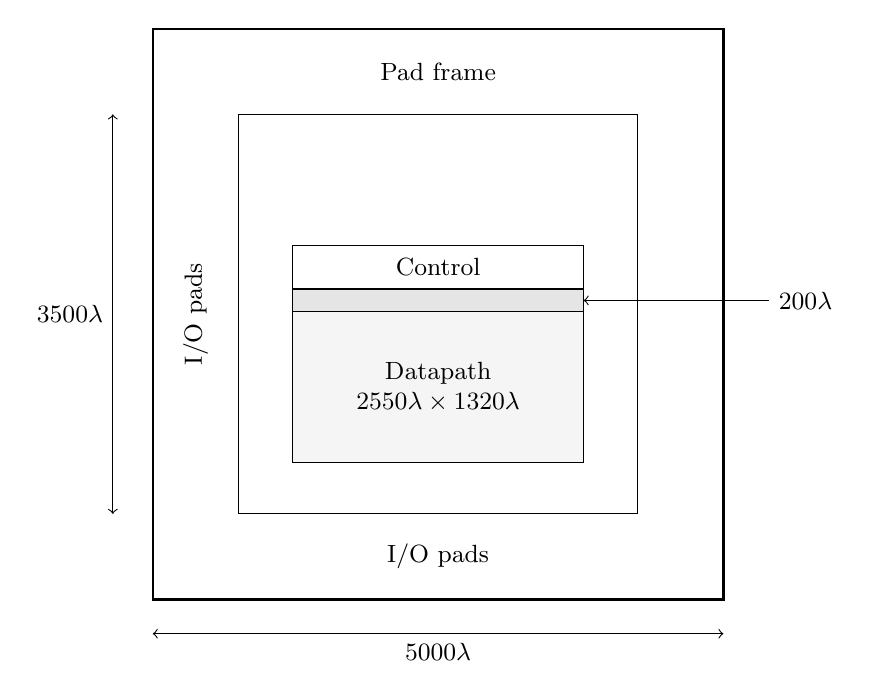
\begin{tikzpicture}[x=0.00145cm,y=0.00145cm,font=\small]
\draw[thick] (0,0) rectangle (5000,5000);
\draw (750,750) rectangle (4250,4250);
\node at (2500,4625) {Pad frame};
\node[rotate=90] at (375,2500) {I/O pads};
\node at (2500,375) {I/O pads};
\draw[fill=gray!8] (1225,1200) rectangle (3775,2520);
\node[align=center] at (2500,1860) {Datapath\\$2550\lambda\times1320\lambda$};
\draw[fill=gray!20] (1225,2520) rectangle (3775,2720);
\draw (1225,2720) rectangle (3775,3100);
\node at (2500,2910) {Control};
\draw[<-] (3775,2620)--(5400,2620) node[right] {$200\lambda$};
\draw[<->] (0,-300)--(5000,-300) node[midway,below] {$5000\lambda$};
\draw[<->] (-350,750)--(-350,4250) node[midway,left] {$3500\lambda$};
\end{tikzpicture}
\end{latin}
\caption{\lr{Floorplan} آموزشی با نسبت ابعاد اصلی کتاب. مستطیل میانی، فضای قابل‌استفاده
داخل \lr{Pad Frame} است. نوار خاکستری کانال کنترل را نشان می‌دهد. جزئیات تک‌تک \lr{Pad}ها حذف شده‌اند
\cite[شکل \secnum{۱.۶۲}]{weste}.}
\label{fig:impl-floorplan}
\end{figure}

\subsection{تبدیل طول و مساحت در مثال کتاب}
در فناوری آموزشی \qty{0.6}{\micro\metre} این مثال، \(\lambda=\qty{0.3}{\micro\metre}\)
است. بنابراین ضلع \(5000\lambda\) برابر \qty{1500}{\micro\metre} یا
\qty{1.5}{\milli\metre} می‌شود. رابطه عمومی تبدیل مساحت چنین است
\begin{equation}
 A_{\mathrm{physical}}=A_{\lambda}\lambda^2.
 \label{eq:impl-area-conversion}
\end{equation}
در این رابطه \(A_{\lambda}\) مقدار عددی مساحت در واحد \(\lambda^2\) است.
چون هر دو بعد طول در \(\lambda\) ضرب می‌شوند، ضریب تبدیل مساحت مربع می‌شود.
در این فناوری، \(1\lambda^2=\qty{0.09}{\micro\metre\squared}\) است.

ابعاد هر \lr{Pad} در کتاب \(750\lambda\times350\lambda\) ذکر شده‌اند.
با کنارگذاشتن حاشیه شعاعی \(750\lambda\) در هر طرف، ضلع فضای داخلی
\(5000-2(750)=3500\lambda\) می‌شود. پس
\begin{align}
 A_{\mathrm{die}}&=(5000\lambda)^2
 =25\times10^6\lambda^2=\qty{2.25}{\milli\metre\squared},\notag\\
 A_{\mathrm{inside}}&=(3500\lambda)^2
 =12.25\times10^6\lambda^2=\qty{1.1025}{\milli\metre\squared}.
 \label{eq:impl-die-core}
\end{align}
مساحت داخل قاب، ظرفیت هندسی موجود را بیان می‌کند. ابعاد بسته پردازنده، شامل دو
بلوک و کانال میان آن‌ها، کوچک‌تر است. با ابعاد گرد‌شده \lr{Floorplan} داریم
\begin{align}
 H_{\mathrm{core}}&=(1320+200+380)\lambda=1900\lambda,\notag\\
 A_{\mathrm{core}}&=(2550)(1900)\lambda^2
 =4.845\times10^6\lambda^2\approx4.8\times10^6\lambda^2.
 \label{eq:impl-core-area}
\end{align}
سهم \lr{Datapath}، کنترل و کانال به‌ترتیب
\(3.366\times10^6\lambda^2\)، \(0.969\times10^6\lambda^2\) و
\(0.510\times10^6\lambda^2\) است. جمع آن‌ها دقیقاً مقدار
\eqref{eq:impl-core-area} را می‌دهد. مقدار فیزیکی متناظر \qty{0.43605}{\milli\metre\squared}
است که برای گزارش تقریبی می‌توان \qty{0.44}{\milli\metre\squared} نوشت.

در این مثال، فضای موردنیاز \lr{Pad Frame} اندازه \lr{Die} را تعیین می‌کند و طراحی
\lr{Pad-limited} است. در طراحی \lr{Core-limited}، اندازه منطق داخلی عامل تعیین‌کننده
مساحت است. کاهش یک بلوک داخلی در حالت اول، تا زمانی که نیاز قاب ثابت بماند،
الزاماً اندازه نهایی \lr{Die} را کاهش نمی‌دهد \cite[صفحه ۴۷]{weste}.

\subsection{گونه‌های ساختار و \lr{Standard Cell}}
کتاب ساختارهای روی تراشه را در گروه‌های \lr{Random Logic}، \lr{Datapath}،
\lr{Array}، \lr{Analog} و \lr{I/O} توضیح می‌دهد \cite[صفحه ۴۸]{weste}.
\lr{Random Logic} اتصال‌های کم‌نظم، مانند \lr{Decoder} منطقی عمومی، دارد.
در \lr{Datapath}، کار مشابه در چند بیت تکرار می‌شود. در \lr{Array}، سلول‌های مشابه
در دو بعد تکرار می‌شوند، مانند \lr{RAM}، \lr{ROM} و \lr{PLA}.
مدار \lr{Analog} و سلول \lr{I/O} به نیازهای الکتریکی و فناوری ویژه خود وابسته‌اند.
تکرار سلولِ طراحی و بررسی‌شده، هزینه طراحی آرایه‌ها را میان نمونه‌های متعدد تقسیم می‌کند.

\lr{Standard Cell} یک سلول کتابخانه‌ای با تابع و هندسه ازپیش‌تعریف‌شده، مانند
\lr{Inverter}، \lr{NAND} یا \lr{Flip-flop}، است. در نمونه کتاب، ریل‌های افقی
تغذیه در \lr{Metal1} عرض \(8\lambda\) و فاصله مرکز تا مرکز \(90\lambda\) دارند.
\lr{nMOS}ها در ناحیه پایین \(40\lambda\) و \lr{pMOS}ها در ناحیه بالای
\(50\lambda\) قرار می‌گیرند. هم‌ترازی ریل و \lr{n-well} امکان اتصال سلول‌های مجاور
از طریق \lr{Abutment} را فراهم می‌کند.

عرض سلول مضربی از \(8\lambda\) است تا تعداد صحیحی مسیر عمودی \lr{Metal2}
داشته باشد. ورودی و خروجی در \lr{Metal2} در دسترس‌اند. \lr{Poly} عمدتاً عمودی و
\lr{Diffusion} و \lr{Metal1} عمدتاً افقی‌اند. اتصال‌های \lr{Substrate} و
\lr{Well} زیر ریل‌ها جا می‌گیرند. فاصله تکرار ردیف‌ها حداقل \(110\lambda\) است.
این اعداد، قواعد کتابخانه آموزشی همان مثال هستند \cite[بخش \secnum{۱.۱۰.۲}]{weste}.

در فرآیند دوفلزی، مسیرهای افقی میان ردیف‌ها به کانال نیاز دارند و تعداد سیم‌ها
ارتفاع کانال را تعیین می‌کند. در مثال سه‌فلزی، \lr{Metal3} افقی با
\lr{Pitch} برابر \(10\lambda\)، روی ارتفاع \(110\lambda\) حدود ۱۱ مسیر فراهم می‌کند.
اگر تقاضای سیم‌کشی در این ظرفیت جا بگیرد، کانال جداگانه می‌تواند حذف شود.
در مثال \lr{MIPS}، جهت‌های غالب \lr{Metal1}، \lr{Metal2} و \lr{Metal3}
به‌ترتیب افقی، عمودی و افقی‌اند. این ترتیب عبور سیم‌ها در لایه‌های مختلف را آسان می‌کند.

کتاب در شکل‌های \secnum{۱.۶۴} و \secnum{۱.۶۵}، نتیجه \lr{Place and Route}
کنترل‌کننده و پردازنده را نشان می‌دهد. نمونه پردازنده در فناوری \qty{130}{\nano\metre}
با هفت لایه فلز، ۲۶ ردیف سلول و حدود \(4\times10^6\lambda^2\) مساحت دارد.
مقایسه تلاش طراحی و سرعت در متن کتاب مربوط به همین زمینه تاریخی است.

\subsection{\lr{Pitch Matching} و \lr{Slice Plan}}
\lr{Pitch} فاصله تکرار یک ساختار است. برای سلول‌هایی که در امتداد یک لبه به هم
می‌چسبند، اندازه و محل اتصال‌های آن لبه باید هماهنگ شوند. این هماهنگی
\lr{Pitch Matching} نام دارد. کوچک‌کردن یک سلول هنگامی که ابعاد نهایی را سلول
همسایه تعیین می‌کند، ممکن است تنها فضای خالی ایجاد کند. بزرگ‌کردن همان سلول نیز
می‌تواند ابعاد همسایه و کل آرایه را افزایش دهد \cite[شکل \secnum{۱.۶۶}]{weste}.

برای نمونه فرضی، چهار سلول با عرض \(w_A\) کنار هم به بلوکی با عرض \(w_B\)
متصل می‌شوند. اگر لبه‌های بیرونی باید هم‌تراز بمانند، عرض موردنیاز ناحیه
\(W=\max(4w_A,w_B)\) است. با \(w_A=20\lambda\) و \(w_B=90\lambda\)،
عرض \(90\lambda\) می‌شود. کاهش \(w_A\) به \(18\lambda\) همچنان همان عرض
نهایی را می‌دهد. برای استفاده از فضای آزاد باید سازمان‌دهی ناحیه نیز بازنگری شود.

\lr{Slice Plan} ترتیب \lr{Wordslice}ها و تخصیص مسیرها در هر \lr{Bitslice} را
پیش از رسم جزئیات مشخص می‌کند. در شکل \secnum{۱.۶۸} کتاب، نقطه روی مسیر بیان می‌کند
که گذرگاه علاوه بر عبور از سلول، در آن سلول مصرف یا تولید می‌شود. پهنای هر جزء با
تعداد مسیر نوشته شده است. بیشترین تراکم این مثال روی \lr{Register File} و برابر
هفت مسیر است \cite[بخش \secnum{۱.۱۰.۴}]{weste}.

جمع عرض اجزای شکل کتاب ۳۱۹ مسیر است. با \lr{Pitch} برابر \(8\lambda\)،
عرض \lr{Datapath} چنین محاسبه می‌شود
\begin{equation}
 W_{\mathrm{data}}=319\times8\lambda=2552\lambda.
 \label{eq:impl-slice-width}
\end{equation}
عدد \(2550\lambda\) در \lr{Floorplan}، مقدار گرد‌شده همین تخمین است.
ارتفاع از هشت \lr{Bitslice}، یک ردیف \lr{Zipper} و سه ردیف \lr{Address Decoder}
ساخته می‌شود. پس با ۱۲ ردیف و فاصله \(110\lambda\)، ارتفاع
\(12(110)\lambda=1320\lambda\) است. فضای خالی ردیف‌های \lr{Decoder} در طراحی
فشرده‌تر می‌تواند برای بخش دیگری مانند کنترل استفاده شود. این تغییر به سازگاری
اتصال و زمان‌بندی نیاز دارد.

\subsection{\lr{Array} و نمونه \lr{PLA}}
\lr{Programmable Logic Array} یا \lr{PLA} توابع به صورت \lr{Sum of Products}
را با دو صفحه پیاده می‌کند. \lr{AND Plane} جمله‌های حاصل‌ضرب و \lr{OR Plane}
ترکیب آن‌ها را می‌سازد. برای نمونه، \(F=ab+ac\) به دو جمله حاصل‌ضرب و یک خروجی
نیاز دارد. در کنترل‌کننده کتاب، این ساختار منطق حالت بعد و خروجی \lr{FSM} را
پیاده می‌کند \cite[بخش \secnum{۱.۱۰.۵}، شکل \secnum{۱.۶۹}]{weste}.

برای قالب آموزشی همان کتاب، هر ورودی دو مسیر عمودی، هر خروجی سه مسیر عمودی و
حاشیه حدود شش مسیر می‌خواهد. هر جمله حاصل‌ضرب حدود یک‌ونیم مسیر افقی و حاشیه
حدود ۱۴ مسیر لازم دارد. اگر \(n_i,n_o,n_p\) به‌ترتیب تعداد ورودی، خروجی و جمله
حاصل‌ضرب و \(p_v,p_h\) فاصله مسیرهای عمودی و افقی باشند، تخمین ساختاری برابر است با
\begin{equation}
 W\approx(2n_i+3n_o+6)p_v,\qquad
 H\approx(1.5n_p+14)p_h.
 \label{eq:impl-pla-estimate}
\end{equation}
فاصله مسیر هر جهت باید از همان قالب سلول تعیین شود. این رابطه رشد عرض با ورودی
و خروجی و رشد ارتفاع با تعداد جمله‌ها را روشن می‌کند.

\lr{PLA} مثال کتاب \(500\lambda\times350\lambda\) است و چهار \lr{Flip-flop}
خارجی ناحیه \(336\lambda\times220\lambda\) دارند. جمع مساحت این دو بخش
\(175000+73920=248920\lambda^2\) می‌شود. مساحت کنترل‌کننده باید سیم‌های ورودی
و خروجی و الزامات جانمایی را نیز در بر بگیرد. برای مقایسه، نمونه کنترل‌کننده حاصل
از ابزار در شکل \secnum{۱.۶۴} ابعاد \(1500\lambda\times400\lambda\) دارد و
بخش بزرگی از آن را کانال‌ها اشغال می‌کنند. این دو سازمان‌دهی و \lr{Floorplan}
بالادستی را با ابعاد و قیود مخصوص خود مقایسه می‌کنیم.

\subsection{تخمین مساحت و دقت اعداد}
تخمین زودهنگام می‌تواند از بلوک مشابه پیشین یا از چگالی تقریبی آغاز شود.
جدول \ref{tab:impl-density} داده‌های جدول \secnum{۱.۱۰} کتاب را با واحد روشن
بازنویسی می‌کند. این اعداد به فناوری، قالب سلول و روش سیم‌کشی وابسته‌اند.
\begin{table}[ht]
\centering
\caption{چگالی‌های تقریبی آموزشی کتاب برای تخمین اولیه \cite[صفحه ۵۲]{weste}.}
\label{tab:impl-density}
\begin{tabularx}{\textwidth}{rX}
\toprule
ساختار & مساحت تقریبی\\
\midrule
\lr{Random Logic} با دو لایه فلز & \(1000\) تا \(1500\lambda^2\) به‌ازای ترانزیستور\\
\lr{Datapath} & \(250\) تا \(750\lambda^2\) به‌ازای ترانزیستور، یا مدل \(6WL+360\lambda^2\)\\
\lr{SRAM} & \(1000\lambda^2\) به‌ازای بیت\\
\lr{DRAM} در فرآیند ویژه آن & \(100\lambda^2\) به‌ازای بیت\\
\lr{ROM} & \(100\lambda^2\) به‌ازای بیت\\
\bottomrule
\end{tabularx}
\end{table}
در مدل \(6WL+360\lambda^2\)، طول‌های \(W,L\) باید با واحد طول سازگار جای‌گذاری
شوند تا \(WL\) مساحت شود. برای حافظه، مساحت بیت‌ها به همراه \lr{Decoder} و مدارهای
جانبی در نظر گرفته می‌شود. تخمین کانال نیز از تعداد مسیر ضرب‌در \lr{Pitch}
آغاز می‌شود. کاهش جزئی سلولی که بارها تکرار می‌شود می‌تواند در سطح کل تراشه اثر
زیادی بگذارد. تخمین محافظه‌کارانه، فضای لازم برای اصلاح و رشد بلوک را فراهم می‌کند.

گاهی چگالی به صورت \lr{kgates/mm²} گزارش می‌شود. کتاب در مثال خود، هر \lr{Gate}
معادل را یک \lr{NAND3} یا \lr{NOR3} شش‌ترانزیستوری می‌گیرد. با این تعریف و
\(\lambda\approx\qty{0.03}{\micro\metre}\)، چگالی
\(160\) تا \(500\) هزار \lr{Gate} در \unit{\milli\metre\squared} به‌ترتیب حدود
\(1160\) تا \(370\lambda^2\) برای هر ترانزیستور می‌دهد
\cite[صفحه ۵۳]{weste}. برای مقدار ۱۶۰ هزار، محاسبه چنین است
\begin{equation}
 a_{\mathrm{tr}}\approx
 \frac{10^6\,\unit{\micro\metre\squared}}
 {160000\times6}\,
 \frac{\lambda^2}{0.03^2\,\unit{\micro\metre\squared}}
 \approx1160\lambda^2.
 \label{eq:impl-density-conversion}
\end{equation}
افزایش چگالی، مساحت متناظر هر ترانزیستور را کاهش می‌دهد. مقایسه دو گزارش چگالی
باید با تعریف یکسان \lr{Gate} و محدوده یکسان سیم‌کشی انجام شود.

\clearpage
\subsection{تمرین‌های پاسخ‌دار \lr{Physical Design}}
\textbf{تمرین ۱.} بلوک فرضی با ۱۰ هزار ترانزیستور و تخمین
\(1000\lambda^2\) برای هر ترانزیستور، در فناوری \(\lambda=\qty{0.1}{\micro\metre}\)
چه مساحتی دارد؟ ابتدا مساحت در واحد \(\lambda^2\) برابر \(10^7\lambda^2\) است.
پس مساحت فیزیکی \(10^7(0.1)^2=10^5\,\unit{\micro\metre\squared}\) یا
\qty{0.1}{\milli\metre\squared} می‌شود. برای فرض مربع‌بودن بلوک، ضلع
\(\sqrt{0.1}\,\unit{\milli\metre}\approx\qty{0.316}{\milli\metre}\) است.
این تخمین باید با محدوده‌ای که چگالی گزارش‌شده پوشش می‌دهد تفسیر شود.

\textbf{تمرین ۲.} برای کانال فرضی ۲۵ مسیر با فاصله \(8\lambda\)، ارتفاع لازم
در مدل کتاب چقدر است؟ حاصل \(25(8)\lambda=200\lambda\) می‌شود.
در \(\lambda=\qty{0.3}{\micro\metre}\)، ارتفاع \qty{60}{\micro\metre} است.
عرض کانال \(2550\lambda\) باشد، مساحت \(510000\lambda^2\) یا
\qty{45900}{\micro\metre\squared} خواهد بود.

\textbf{تمرین ۳.} اگر عرض \lr{Datapath} از ۳۱۹ به ۳۰۰ مسیر برسد و ارتفاع
۱۲ ردیفی ثابت بماند، کاهش مساحت چقدر است؟ عرض جدید \(2400\lambda\) و کاهش
عرض \((319-300)8\lambda=152\lambda\) است. کاهش مساحت برابر
\(152(1320)\lambda^2=200640\lambda^2\)، یعنی حدود ۶ درصد مساحت اولیه
\(2552(1320)\lambda^2\)، می‌شود. تغییر مساحت کل \lr{Die} به عامل تعیین‌کننده
ابعاد نهایی نیز وابسته است.
\clearpage

\section{بررسی درستی طراحی}
\label{sec:book-verification}
\subsection{رابطه میان \lr{Specification} و نمایش‌های طراحی}
\lr{Verification} بررسی می‌کند که طراحی با رفتار و محدودیت‌های مورد انتظار
سازگار باشد. \lr{Specification} باید رفتار خروجی، شرایط ورودی، \lr{Reset}،
زمان‌بندی و سایر قیود لازم را مشخص کند. با دقیق‌ترشدن نمایش، تعداد جزئیات و هزینه
تحلیل افزایش می‌یابد. کتاب برای مدیریت این هزینه، بررسی عملکرد در سطوح بالاتر و
بررسی سازگاری میان نمایش‌های متوالی را توضیح می‌دهد
\cite[بخش \secnum{۱.۱۱}، شکل \secnum{۱.۷۰}]{weste}.

در سطح معماری، مدل رفتاری مانند برنامه \lr{C} با تعریف معماری سنجیده می‌شود.
در سطح منطق، \lr{HDL} با ورودی و خروجی مورد انتظار بررسی می‌شود. در مرحله مدار،
عملکرد شبکه ترانزیستور با تابع منطقی مقایسه می‌شود. در مرحله فیزیکی، اتصال‌های
استخراج‌شده از \lr{Layout} با \lr{Schematic} مقایسه می‌شوند. در کنار این زنجیره،
مدار و \lr{Layout} باید قیود زمان‌بندی و توان را برآورده کنند.

برای نمونه، اگر نیاز سیستم جمع هشت‌بیتی با \lr{Carry-out} باشد، رفتار مرجع باید
جمع کامل ۹ بیتی را مشخص کند. سپس خروجی هشت‌بیتی، هشت بیت کم‌ارزش نتیجه و
\lr{Carry-out} بیت نهم است. اگر تعریف علامت‌دار بودن داده یا رفتار \lr{Overflow}
مبهم بماند، پاسخ مورد انتظار آزمون نیز مبهم می‌شود.

\subsection{\lr{Testbench} و انتخاب ورودی‌ها}
\lr{Testbench} محیطی است که \lr{Device Under Test} یا \lr{DUT} را نمونه‌سازی
می‌کند، ورودی‌ها را اعمال می‌کند و پاسخ را با مرجع مقایسه می‌کند. یک \lr{Test Vector}
می‌تواند شامل ورودی و پاسخ مورد انتظار باشد. در مدار ترتیبی، زمان اعمال ورودی،
\lr{Clock}، \lr{Reset} و وضعیت قبلی نیز بخشی از سناریو هستند
\cite[صفحه ۵۳]{weste}.

برای تابع ترکیبی با \(n\) ورودی دودویی، تعداد حالت‌ها \(2^n\) است، زیرا برای هر
ورودی دو انتخاب مستقل داریم. \lr{Carry} سه‌ورودی ۸ حالت دارد. جمع‌کننده هشت‌بیتی
با دو عملوند هشت‌بیتی و یک \lr{Carry-in}، تعداد
\(2^{8+8+1}=131072\) حالت دارد. با افزایش ورودی‌ها، بررسی کامل به‌سرعت پرهزینه
می‌شود. برای مدار ترتیبی، ترتیب ورودی‌ها و حالت داخلی نیز باید بررسی شوند.

در نمونه آموزشی، برای جمع‌کننده ورودی‌های صفر، بیشینه مقدار، تولید و انتشار
\lr{Carry} و الگوهای مکمل ارزش بررسی دارند. در پردازنده، \lr{Reset}، هر نوع دستور،
شاخه گرفته‌شده و گرفته‌نشده و مرز نشانی‌ها باید طبق تعریف معماری آزموده شوند.
پاسخ مرجع باید از صورت مسئله و محاسبه مستقل به دست آید. کپی همان عبارت اشتباه
از طراحی به مرجع می‌تواند همان خطا را در هر دو حفظ کند.

\lr{Post-synthesis Netlist} را می‌توان با بردارهای آزمون قبلی شبیه‌سازی کرد.
برای شبکه ترانزیستور نیز آزمون عملکرد ممکن است. در مدار ترتیبی، ترتیب رخدادها و
\lr{Race Condition} اهمیت پیدا می‌کند. ابزار \lr{Formal Verification} نیز می‌تواند
تحت فرض‌ها و مدل تعریف‌شده، هم‌ارزی تابع یا خاصیت را بررسی کند.
کیفیت فرض‌ها و پوشش حالت‌ها بر معنای نتیجه اثر می‌گذارد.

\subsection{\lr{DRC}، \lr{LVS}، \lr{ERC} و تحلیل الکتریکی}
\lr{Design Rule Check} یا \lr{DRC} هندسه را با قواعد فناوری مقایسه می‌کند، مانند
حداقل عرض، فاصله و پوشش اتصال. \lr{Layout Versus Schematic} یا \lr{LVS} بررسی
می‌کند که ترانزیستورها و اتصال‌های استخراج‌شده از \lr{Layout} با مدار مرجع سازگار
باشند. \lr{Electrical Rule Check} یا \lr{ERC} برای یافتن مسئله‌های الکتریکی
تعریف‌شده در مجموعه قواعد به کار می‌رود. کتاب به مشکلاتی مانند نویز یا فرسودگی
زودهنگام اشاره می‌کند \cite[صفحه ۵۳]{weste}.

جدول \ref{tab:impl-verification} مثال‌هایی از ارتباط خطا و بررسی مناسب را نشان می‌دهد.
یک مسئله ممکن است در بیش از یک بررسی آشکار شود و توان کشف هر ابزار به مدل و قواعدش وابسته است.
\begin{table}[ht]
\centering
\caption{نمونه ارتباط مسئله طراحی با بررسی لازم.}
\label{tab:impl-verification}
\begin{tabularx}{\textwidth}{rX}
\toprule
مسئله & بررسی مرتبط\\
\midrule
اشتباه در تابع \lr{Carry} & مقایسه رفتاری، جدول کامل یا بررسی هم‌ارزی\\
سیم با عرض کمتر از حد مجاز & \lr{DRC} با قواعد فناوری\\
اتصال خروجی به گره داخلی اشتباه & \lr{LVS} در برابر مدار مرجع\\
اتصال الکتریکی نامناسب تغذیه یا \lr{Body} & \lr{ERC} و بررسی اتصال با قواعد مرتبط\\
رسیدن خروجی پس از مهلت لازم & تحلیل زمان‌بندی با مدل مناسب مدار و سیم\\
مصرف توان بیشتر از بودجه & تحلیل توان با تحریک، فعالیت و مدل معتبر\\
\bottomrule
\end{tabularx}
\end{table}

اگر هندسه قانونی باشد اما دو گره منطقی جابه‌جا شده باشند، ممکن است
\lr{DRC} بدون خطای هندسی پایان یابد و \lr{LVS} اختلاف اتصال را پیدا کند.
اگر اتصال با مرجع برابر باشد اما خود مرجع تابع اشتباه داشته باشد، مقایسه رفتاری
با \lr{Specification} لازم است. برای بررسی سرعت و توان نیز مقاومت و خازن سیم،
اندازه ترانزیستور، ولتاژ و شرایط مدل‌شده اهمیت دارند.

\subsection{تمرین‌های پاسخ‌دار \lr{Verification}}
\textbf{تمرین ۱.} در گیت \lr{NAND2}، خروجی در \lr{Layout} به \(V_{DD}\) اتصال
پیدا کرده است. آزمون عملکرد چه ورودی‌ای را باید حتماً اعمال کند؟
برای \(a=b=1\)، پاسخ مرجع صفر است. خروجی ثابت یک اختلاف را آشکار می‌کند.
سه حالت دیگر خروجی مرجع یک دارند و این خطا را در مدل خروجی ثابت نشان نمی‌دهند.
\lr{LVS} نیز باید اختلاف اتصال با مدار صحیح را بررسی کند.

\textbf{تمرین ۲.} مدار تابع درست را با تأخیر \qty{2}{\nano\second} تولید می‌کند،
ولی مهلت داده‌شده \qty{1.5}{\nano\second} است. نتیجه چیست؟
شرط عملکرد منطقی برآورده شده، اما قید زمان‌بندی \qty{0.5}{\nano\second} نقض شده است.
برای اعلام موفقیت باید هر دو شرط تابع و مهلت برقرار باشند.

\textbf{تمرین ۳.} آیا یک آزمون موفق برنامه \lr{Fibonacci}، همه حالت‌های پردازنده
را پوشش می‌دهد؟ این برنامه تنها توالی مشخصی از دستورها، داده‌ها و شاخه‌ها را طی
می‌کند. برای پوشش نیازهای دیگر باید سناریوهای متناسب با همان نیازها افزوده شود.
مثلاً صحت \lr{Reset}، دستور استفاده‌نشده و حالت مرزی \lr{Branch} به بررسی مربوط خود نیاز دارد.
\clearpage

\section{ساخت، \lr{Packaging} و \lr{Testing}}
\label{sec:book-manufacturing}
\subsection{\lr{Tapeout}، \lr{Mask} و تقسیم هزینه ساخت}
پس از نهایی‌شدن طراحی و بررسی‌های لازم، توصیف هندسه ماسک‌ها برای ساخت تحویل
داده می‌شود. این مرحله \lr{Tapeout} نام دارد. نام آن از روش تاریخی تحویل داده روی
نوار مغناطیسی آمده است. کتاب قالب‌های \lr{Caltech Interchange Format} یا
\lr{CIF} و \lr{Calma GDS II Stream Format} یا \lr{GDS} را معرفی می‌کند
\cite[بخش \secnum{۱.۱۲}]{weste}.

\lr{Mask} الگوی لازم برای انتقال هندسه یک مرحله از فرآیند را فراهم می‌کند.
کتاب روش ساخت الگوی کروم روی شیشه با پرتو الکترونی را توضیح می‌دهد.
هزینه ماسک و تجهیز خط تولید، بخش مهمی از هزینه ثابت ساخت است.
متن سال ۲۰۱۱ برای مثال‌های \qty{180}{\nano\metre} و \qty{65}{\nano\metre}
به‌ترتیب حدود ۲۵۰ هزار و ۳ میلیون دلار هزینه مجموعه ماسک ذکر می‌کند.
این مقادیر، مثال تاریخی همان کتاب‌اند.

در \lr{Multi-project Wafer}، چند طراحی کوچک از مجموعه مشترکی از ماسک‌ها استفاده
می‌کنند تا هزینه ثابت میان مشتریان تقسیم شود. کتاب خدمات \lr{MOSIS}،
\lr{EUROPRACTICE} و \lr{VDEC} را در زمینه زمان انتشار معرفی می‌کند.
در مدل آموزشی فرضی، اگر هزینه ثابت مشترک \(K\) میان \(N\) طراحی با سهم برابر
تقسیم شود، سهم هر طراحی \(K/N\) است. هزینه عملی به سهم سطح، فرآیند، تعداد نمونه،
\lr{Packaging} و شرایط خدمات وابسته است.

\lr{Fab} کارخانه ساخت و \lr{Foundry} تأمین‌کننده خدمات ساخت است.
شرکت \lr{Fabless} طراحی را انجام می‌دهد و ساخت را به کارخانه طرف قرارداد می‌سپارد.
کتاب هزینه بالای تأسیس کارخانه و اهمیت اقتصادی این تقسیم کار را توضیح می‌دهد.

\subsection{از \lr{Wafer} تا \lr{Die}}
روی یک \lr{Wafer} سیلیکونی، تعداد زیادی نسخه مدار هم‌زمان ساخته می‌شوند.
مراحل تکراری رسوب‌دهی، ماسک‌گذاری، \lr{Etch} و \lr{Implant} همان هندسه و
ساختار افزاره را ایجاد می‌کنند که در بخش ساخت مقدماتی آموختیم.
کتاب قطرهای \qty{150}{\milli\metre} تا \qty{300}{\milli\metre} و زمان بازگشت
تا حدود ۱۰ هفته را برای زمینه صنعتی زمان خود شرح می‌دهد \cite[صفحه ۵۴]{weste}.

در \lr{Clean Room}، فیلتر هوا و پوشش کارکنان، ورود ذرات آلاینده را کاهش می‌دهد.
یک ذره کوچک می‌تواند بخشی از الگو را خراب کند و اتصال باز یا اتصال کوتاه بسازد.
پس از فرآوری، \lr{Wafer} به قطعه‌های \lr{Die} بریده می‌شود. هندسه نهایی قطعه،
تعداد و محل اتصال‌ها و نیاز حرارتی، در انتخاب \lr{Package} نقش دارند.

\subsection{\lr{Wire Bonding} و \lr{Flip-chip}}
\lr{Package} اتصال قابل‌استفاده با محیط بیرونی و حفاظت مکانیکی قطعه را فراهم
می‌کند و در دفع گرما و رفتار الکتریکی نیز نقش دارد. مثال \lr{MIPS} کتاب، قطعه
\qty{1.5}{\milli\metre} در \qty{1.5}{\milli\metre} را در \lr{Dual-inline Package}
یا \lr{DIP} با ۴۰ پایه نشان می‌دهد. در \lr{Wire Bonding}، سیم‌های نازک طلا
\lr{Pad}های قطعه را به \lr{Lead Frame} بسته وصل می‌کنند
\cite[شکل \secnum{۱.۷۳} و صفحه ۵۵]{weste}.

در \lr{Flip-chip}، اتصال‌های لحیمی کوچک روی سطح قطعه ایجاد می‌شوند و قطعه
روبه‌پایین به زیرلایه متصل می‌شود. امکان توزیع اتصال‌ها در سطح تراشه، ظرفیت اتصال
را افزایش می‌دهد. حذف سیم \lr{Bond Wire} سهم القایی آن سیم را از مسیر برمی‌دارد.
رفتار الکتریکی نهایی همچنان به کل مسیر اتصال و بسته وابسته است.
کتاب معیارهای هزینه، تعداد پایه، پهنای باند پایه، انتقال توان و قابلیت اطمینان را
برای مقایسه بسته‌ها مطرح می‌کند و جزئیات را به فصل ۱۳ ارجاع می‌دهد.

\subsection{آزمون قطعه ساخته‌شده و \lr{BIST}}
\lr{Testing} قطعه ساخته‌شده را با معیار پذیرش می‌سنجد تا نمونه‌های دارای عیب
شناسایی شوند. حتی با طراحی صحیح، نقص ساخت یا آلودگی می‌تواند قطعه معیوب ایجاد کند.
آزمون به دسترسی ورودی‌ها، مشاهده پاسخ‌ها، سرعت موردنظر و هزینه زمانی دستگاه
آزمون وابسته است \cite[صفحه ۵۵]{weste}.

در \lr{Built-in Self-test} یا \lr{BIST}، مدارهای کمکی روی تراشه بخشی از تولید
تحریک و بررسی پاسخ را انجام می‌دهند. هدف معرفی‌شده در کتاب کاهش زمان لازم
دستگاه آزمون خارجی است. این انتخاب، منطق و مساحت کمکی می‌خواهد.
پوشش عیب به روش تولید الگو و تحلیل پاسخ وابسته است.
معیار آزمون باید با عیب‌هایی که قصد کشفشان را داریم متناسب باشد.

برای تحلیل اقتصادی ساده، \lr{Yield} را نسبت تعداد قطعات سالم به تعداد قطعات
ساخته‌شده تعریف می‌کنیم. اگر به فرض ۱۰۰۰ قطعه ساخته شود و ۸۵۰ قطعه معیار پذیرش
را برآورده کنند، \(Y=850/1000=0.85\)، یعنی ۸۵ درصد است.
اگر هزینه مفروض همین مرحله \(K\) باشد، هزینه سرشکن‌شده هر قطعه سالم در این مدل
\begin{equation}
 C_{\mathrm{good}}=\frac{K}{N_{\mathrm{good}}}
 =\frac{K}{YN_{\mathrm{total}}}
 \label{eq:impl-yield-cost}
\end{equation}
خواهد بود. \(N_{\mathrm{total}}\) تعداد کل و \(N_{\mathrm{good}}\) تعداد سالم است.
با ثابت‌بودن هزینه و تعداد ساخت، کاهش \lr{Yield} هزینه هر قطعه سالم را افزایش می‌دهد.
این مثال افزوده، مدل سرشکن‌کردن یک هزینه مشخص است. هزینه‌های مراحل دیگر باید
در مدل اقتصادی کامل خود لحاظ شوند.

\subsection{تمرین‌های پاسخ‌دار ساخت و آزمون}
\textbf{تمرین ۱.} هزینه فرضی یک مرحله برای ۱۰۰۰ قطعه، ۲۰ هزار واحد پول است.
با \lr{Yield} برابر ۸۰ درصد، هزینه همان مرحله برای هر قطعه سالم چقدر می‌شود؟
تعداد سالم \(0.8(1000)=800\) و هزینه واحد \(20000/800=25\) واحد پول است.
با \lr{Yield} برابر ۵۰ درصد، هزینه \(20000/500=40\) واحد پول می‌شود.

\textbf{تمرین ۲.} برای عیب خروجی گیرکرده روی صفر در \lr{Carry}، چه ورودی‌ای مناسب است؟
مثلاً \(a=b=1,c=0\) پاسخ مرجع یک دارد و عیب را در مدل گیرکردن خروجی آشکار می‌کند.
ورودی \(0,0,0\) پاسخ مرجع صفر دارد و این عیب خاص را آشکار نمی‌کند.
همان منطق انتخاب تحریک در \lr{Testbench} نیز کاربرد دارد.

\textbf{تمرین ۳.} اگر \lr{LVS} و آزمون عملکرد پیش از ساخت موفق باشند، قطعه ساخته‌شده
چه بررسی دیگری می‌خواهد؟ شرایط ساخت هر نمونه می‌تواند نقص ایجاد کند، بنابراین
آزمون قطعه با معیارهای عملکرد و کیفیت تعیین‌شده لازم است. صحت اتصال استخراج‌شده،
صحت رفتار مدل و سلامت نمونه فیزیکی، هر یک به شواهد مناسب خود وابسته‌اند.

\subsection{پیوند این بخش با مدل‌های فصل ۲}
برای محاسبه دقیق‌تر تأخیر باید بدانیم جریان ترانزیستور چگونه به
\(V_{GS}\)، \(V_{DS}\)، \(V_{BS}\)، \(W\) و \(L\) وابسته است.
برای محاسبه بار باید خازن‌های \lr{Gate}، \lr{Diffusion} و سیم را بشناسیم.
برای ارزیابی حالت منطقی پایدار نیز رابطه ورودی و خروجی \lr{Inverter} اهمیت دارد.
بخش‌های آغازین فصل ۲ این مدل‌های افزاره را می‌سازند و بخش‌های بعدی اثرهای غیرایده‌آل
و مشخصه‌های \lr{DC} را به آن‌ها اضافه می‌کنند.
\clearpage

\section*{جمع‌بندی اهداف طراحی و هزینه}
\phantomsection
\addcontentsline{toc}{section}{جمع‌بندی اهداف طراحی و هزینه}
\label{sec:book-objectives}
جمع‌بندی فصل ۱ کتاب چهار هدف \lr{Reliability}، \lr{Performance}، \lr{Power}
و \lr{Cost} را کنار هم قرار می‌دهد \cite[صفحات چاپی ۵۵ و ۵۶]{weste}.
\lr{Reliability} به عملکرد قابل‌قبول در شرایط و طول عمر مورد انتظار مربوط است.
ولتاژ و دمای مجاز، بخشی از این شرایط‌اند.
\lr{Performance} به زمان انجام کار و توان عملیاتی وابسته است و با فرکانس
\lr{Clock} و میزان موازی‌سازی ارتباط دارد.
توان، محدودیت حرارتی و مصرف انرژی را به انتخاب مدار و فعالیت آن پیوند می‌دهد.
هزینه نیز از تلاش طراحی، ماسک و تولید هر قطعه اثر می‌پذیرد.

\subsection*{هزینه ثابت و هزینه هر قطعه}
\lr{Nonrecurring Engineering} یا \lr{NRE} هزینه‌هایی مانند طراحی و تهیه ماسک
را دربرمی‌گیرد. برای مدل اقتصادی آموزشی، \(K\) را هزینه ثابت، \(c\) را هزینه
تولید هر قطعه و \(N>0\) را تعداد قطعه می‌نامیم.
با فرض ثابت‌بودن \(c\) و لحاظ‌شدن شرایط تولید در همین ضریب، هزینه کل و میانگین برابرند با
\begin{equation}
 C_{\mathrm{total}}=K+Nc,\qquad
 C_{\mathrm{unit}}=\frac{K}{N}+c.
 \label{eq:booklet-nre}
\end{equation}
با افزایش تعداد تولید، سهم هزینه ثابت در هر قطعه کاهش می‌یابد.
کتاب این سازوکار را در مقایسه فناوری با هزینه مهندسی بالا و فناوری بالغ‌تر
توضیح می‌دهد. هزینه واقعی به مساحت، فرآیند، \lr{Yield}، بسته‌بندی و شرایط تولید
وابسته است. اعداد نمونه این پاراگراف برای تحلیل روش فرض می‌شوند.

دو انتخاب فرضی \(A\) و \(B\) با داده‌های
\(K_A=100000\)، \(c_A=5\)، \(K_B=400000\) و \(c_B=2\)، همگی در واحد پول
سازگار، را در نظر بگیرید.
برای \(N=10000\)، میانگین‌ها \(100000/10000+5=15\) و
\(400000/10000+2=42\) واحد پول‌اند.
برای یافتن تعداد برابری، دو رابطه را برابر می‌کنیم
\begin{equation}
 \frac{100000}{N}+5=\frac{400000}{N}+2
 \quad\Longrightarrow\quad
 3=\frac{300000}{N}
 \quad\Longrightarrow\quad N=100000.
 \label{eq:booklet-cost-crossover}
\end{equation}
در این تعداد، هر دو میانگین ۶ واحد پول می‌شوند.
برای تولید کمتر، \(A\) و برای تولید بیشتر، \(B\) در همین فرض‌ها هزینه میانگین
کمتری دارد. این مثال از مفهوم هزینه ثابت در جمع‌بندی کتاب بسط داده شده است.

\subsection*{پیوند مدل‌های درس با تصمیم طراحی}
انتخاب شبکه منطقی و اندازه ترانزیستور، جریان و ظرفیت را تغییر می‌دهد.
این دو کمیت، زمان شارژ و تخلیه را تعیین می‌کنند.
انتخاب \lr{Layout}، طول سیم، مساحت پیوندها و فضای سیم‌کشی را تغییر می‌دهد.
روش ساخت و بسته‌بندی نیز بر محدودیت الکتریکی، هزینه و قابلیت اطمینان اثر دارند.
برای ارزیابی یک تصمیم، باید فرض عملکرد، معیار زمان، بودجه توان و مدل فیزیکی
مورد استفاده مشخص باشد.
فصل ۲ این جزوه، مدل جریان و ظرفیت لازم برای آغاز این محاسبه را فراهم می‌کند.
\clearpage


\chapter{مدل جریان و ظرفیت ترانزیستور \lr{MOS}}
\label{chap:mos-theory}
در این فصل، بخش‌های \secnum{۲.۱} تا \secnum{۲.۳} کتاب با استخراج روابط و
کنترل شرط‌های اعتبار مطالعه می‌شوند. نمادهای کوچک \(V_{gs},I_{ds}\) در بحث
مقدماتی و نمادهای \(V_{GS},I_{DS}\) در استخراج تفصیلی، به یک کمیت اشاره دارند.
برای \lr{pMOS}، قرارداد بزرگی مثبت و قرارداد علامت‌دار به‌صراحت معرفی می‌شوند.
\section{ساختار و عملکرد فیزیکی \lr{MOS}}
\label{sec:book-mos-structure}
\subsection{\lr{Silicon}، \lr{Dopant} و حامل متحرک}
اتم \lr{Silicon} چهار الکترون ظرفیت دارد و در شبکه بلوری با همسایه‌ها پیوند
تشکیل می‌دهد. هدایت الکتریکی به وجود حامل‌های متحرک وابسته است.
در دمای غیرصفر، \lr{Silicon} خالص نیز می‌تواند الکترون و \lr{Hole} ناشی از
برانگیزش گرمایی داشته باشد. افزودن مقدار کنترل‌شده ناخالصی، یا \lr{Doping}،
تعداد و نوع حامل غالب را تغییر می‌دهد. اسلایدهای ۲ و ۳ این مقدمه را به صورت
تصویر شبکه و ناخالصی نشان می‌دهند \cite{mos}.

در \lr{n-type}، ناخالصی \lr{Donor} از گروه پنج، مانند \lr{Arsenic}، یک الکترون
اضافی در اختیار هدایت می‌گذارد. پس از آزادشدن الکترون، یون ناخالصی مثبت در شبکه
باقی می‌ماند. در \lr{p-type}، ناخالصی \lr{Acceptor} از گروه سه، مانند
\lr{Boron}، کمبود الکترونی ایجاد می‌کند که به صورت \lr{Hole} توصیف می‌شود.
حرکت پی‌درپی الکترون‌های پیوندی برای پرکردن این جای خالی، مانند جابه‌جایی
حاملی با بار مثبت دیده می‌شود. یون‌های ناخالصی در شبکه ثابت‌اند، اما حامل‌ها متحرک‌اند.

در \lr{n-type}، الکترون‌ها و در \lr{p-type}، \lr{Hole}ها حامل غالب‌اند.
\lr{Doping} معمولاً ماده را در مقیاس حجمی تقریباً خنثی نگه می‌دارد، زیرا بار
حامل‌های متحرک و یون‌ها یکدیگر را جبران می‌کنند. در ناحیه \lr{Depletion}،
خارج‌شدن حامل‌های متحرک، بار یون‌های ثابت را آشکار می‌کند.
این توضیح، معنای دقیق‌تر تقریب «نبود حامل آزاد» در مدل مقدماتی اسلاید ۳ و
متن ساده‌شده صفحه ۶۲ کتاب را فراهم می‌کند.

\subsection{پیوند \lr{p-n} و اتصال \lr{Body}}
تماس ناحیه \lr{p-type} و \lr{n-type} یک پیوند \lr{p-n} می‌سازد.
در مدل دیودی، سمت \lr{p}، \lr{Anode} و سمت \lr{n}، \lr{Cathode} است.
وقتی ولتاژ سمت \lr{p} نسبت به سمت \lr{n} افزایش کافی داشته باشد، پیوند
\lr{Forward-biased} می‌شود. با منفی‌ترشدن سمت \lr{p} نسبت به سمت \lr{n}،
پیوند \lr{Reverse-biased} است و جریان نشتی کوچکی دارد. این مدل مقدماتی
در اسلاید ۴ معرفی شده است \cite{mos}.

در \lr{nMOS}، دو ناحیه \(n^+\) داخل \lr{Body} نوع \lr{p} قرار دارند.
هر یک با \lr{Body} پیوند دیودی دارد. با اتصال \lr{Body} به زمین و ولتاژهای
نامنفی \lr{Source} و \lr{Drain}، این پیوندها بایاس صفر یا معکوس دارند.
در \lr{pMOS}، ناحیه‌های \(p^+\) داخل \lr{Body} نوع \lr{n} هستند و معمولاً
\lr{Body} به بالاترین تغذیه وصل می‌شود. این اتصال پیوندها را در شرایط معمول
مدار از هدایت مستقیم دور نگه می‌دارد \cite[صفحات ۶۲ تا ۶۴]{weste}.

علامت \(+\) در \(n^+\) یا \(p^+\) بیانگر شدت بیشتر \lr{Doping} است.
در ساختمان \lr{MOS}، مسیر کنترل‌شده جریان از لایه زیر \lr{Gate} عبور می‌کند.
بایاس ناخواسته پیوند \lr{Body} می‌تواند مسیر دیگری برای جریان ایجاد کند، بنابراین
پایانه چهارم در بررسی مدار اهمیت دارد.

\subsection{پشته \lr{MOS} و سه وضعیت سطح \lr{Silicon}}
نام کامل \lr{MOS}، عبارت \lr{Metal-Oxide-Semiconductor} است.
لایه \lr{Gate} رسانا، لایه میانی \lr{Gate Oxide} عایق و لایه زیرین نیمه‌رسانای
\lr{Body} است. کتاب به کاربرد تاریخی \lr{Metal Gate}، استفاده از
\lr{Polysilicon} و بازگشت \lr{Metal Gate} در فناوری‌های مورد بحث خود اشاره می‌کند
\cite[صفحه ۶۱]{weste}. عایق میان \lr{Gate} و سطح، امکان کنترل بار سطح با میدان
الکتریکی را فراهم می‌کند.

برای دیدن سه وضعیت سطح، ابتدا ساختار \lr{MOS Capacitor} با \lr{Body} نوع
\lr{p} و متصل به زمین را در نظر می‌گیریم. توصیف ساده کتاب، اثر اختلاف
\lr{Work Function} و بار ثابت اکسید را در نمودار مقدماتی کنار می‌گذارد.
در مدل دقیق، محل آغاز این وضعیت‌ها نسبت به صفر ولتاژ به \lr{Flat-band Voltage}
و پارامترهای ساخت وابسته است. شکل \ref{fig:mos-surface} سه حالت مقدماتی را نشان می‌دهد.

\begin{figure}[ht]
\centering
\begin{latin}
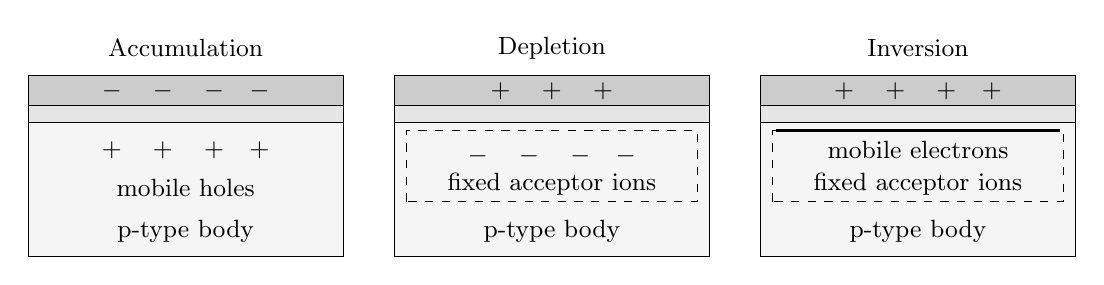
\begin{tikzpicture}[x=1cm,y=1cm,font=\small]
\foreach \x/\title in {0/Accumulation,4.65/Depletion,9.3/Inversion}{
 \draw[fill=gray!8] (\x,0) rectangle +(4,1.7);
 \draw[fill=gray!20] (\x,1.7) rectangle +(4,0.22);
 \draw[fill=gray!40] (\x,1.92) rectangle +(4,0.38);
 \node at (\x+2,2.65) {\title};
 \node at (\x+2,0.32) {p-type body};
}
\node at (2,2.1) {$-\quad-\quad-\quad-$};
\node at (2,1.35) {$+\quad+\quad+\quad+$};
\node at (2,0.87) {mobile holes};
\node at (6.65,2.1) {$+\quad+\quad+$};
\draw[dashed] (4.8,0.7) rectangle (8.5,1.6);
\node at (6.65,1.28) {$-\quad-\quad-\quad-$};
\node at (6.65,0.92) {fixed acceptor ions};
\node at (11.3,2.1) {$+\quad+\quad+\quad+$};
\draw[dashed] (9.45,0.7) rectangle (13.15,1.6);
\draw[very thick] (9.5,1.6)--(13.1,1.6);
\node at (11.3,1.36) {mobile electrons};
\node at (11.3,0.92) {fixed acceptor ions};
\end{tikzpicture}
\end{latin}
\caption{بازنمایی آموزشی سه وضعیت سطح \lr{MOS Capacitor} بر پایه شکل
\secnum{۲.۲} کتاب و اسلاید ۹. نوار میانی نازک، اکسید و نوار بالایی، \lr{Gate} است.
علامت‌های بار شماتیک‌اند و تعداد واقعی حامل‌ها را نشان نمی‌دهند \cite{weste,mos}.}
\label{fig:mos-surface}
\end{figure}

در \lr{Accumulation}، ولتاژ منفی \lr{Gate}، \lr{Hole}های مثبت را به سطح
جذب می‌کند. تراکم حامل غالب نزدیک سطح بیشتر می‌شود.
در \lr{Depletion}، ولتاژ مثبت کوچک \lr{Gate}، \lr{Hole}ها را از سطح دور
می‌کند و ناحیه‌ای با بار یون‌های منفی ثابت \lr{Acceptor} باقی می‌ماند.
در \lr{Inversion}، ولتاژ مثبت کافی، الکترون‌ها را به نزدیکی سطح می‌آورد و
لایه‌ای با حامل غالب الکترونی روی \lr{Body} نوع \lr{p} تشکیل می‌شود.
نوع حامل غالب در سطح تغییر می‌کند، درحالی‌که نوع \lr{Doping} کل \lr{Body} ثابت است.

\lr{Threshold Voltage} یا \(V_t\)، مرز قراردادی تشکیل \lr{Strong Inversion}
در این مدل است. مقدار آن به ساختار و \lr{Doping}، ضخامت اکسید و بایاس بستگی دارد.
در ترانزیستور \lr{Enhancement-mode nMOS} این درس، \(V_{tn}>0\) فرض می‌شود.
کتاب امکان مهندسی آستانه منفی را نیز یادآوری می‌کند.
در استخراج مقدماتی، \(V_t\) ثابت است و اثر بایاس \lr{Body} در بخش
\secnum{۲.۴} بررسی خواهد شد.

\subsection{پایانه‌ها، نمادها و جهت جریان}
چهار پایانه افزاره \lr{Gate}، \lr{Source}، \lr{Drain} و \lr{Body} هستند.
نماد سه‌پایانه اتصال \lr{Body} را به طور ضمنی نشان می‌دهد و در نماد چهارپایانه،
این اتصال آشکار است. کتاب در شکل \secnum{۲.۱} چند قرارداد رسم را نشان می‌دهد.
در نماد متداول اسلایدها، حباب روی \lr{Gate} رفتار معکوس \lr{pMOS} را مشخص می‌کند.
هنگام خواندن شکل، نوع افزاره و اتصال \lr{Body} را هم‌زمان بررسی می‌کنیم
\cite[صفحه ۶۱]{weste}.

هر ولتاژ دوپایانه‌ای، اختلاف پتانسیل پایانه اول و دوم است. تعریف‌ها چنین‌اند
\begin{equation}
 V_{GS}=V_G-V_S,\qquad V_{GD}=V_G-V_D,\qquad
 V_{DS}=V_D-V_S.
 \label{eq:mos-terminal-voltages}
\end{equation}
با کم‌کردن دو ولتاژ اول، \(V_G\) حذف می‌شود و داریم
\begin{equation*}
 V_{GS}-V_{GD}=(V_G-V_S)-(V_G-V_D)=V_D-V_S=V_{DS}.
\end{equation*}
این رابطه همان اسلاید ۱۰ است. برابرگرفتن \(V_{GS}\) با \(V_G\) هنگامی معتبر است
که \(V_S=0\) باشد.

در مدل متقارن مورد استفاده، برای \lr{nMOS} پایانه کم‌پتانسیل‌تر را
\lr{Source} می‌گیریم تا \(V_{DS}\ge0\) باشد. الکترون‌ها از \lr{Source} به
\lr{Drain} حرکت می‌کنند. به دلیل بار منفی الکترون، جریان قراردادی مثبت
\(I_{DS}\) از \lr{Drain} به \lr{Source} است. در \lr{pMOS}،
\lr{Source} پایانه پرپتانسیل‌تر و حرکت \lr{Hole} و جریان قراردادی از
\lr{Source} به \lr{Drain} است \cite[صفحه ۶۴]{weste}.

\subsection{تشخیص \lr{Cutoff}، \lr{Linear} و \lr{Saturation}}
برای \lr{nMOS} با \(V_{tn}>0\)، اگر \(V_{GS}<V_{tn}\) باشد، کانال
\lr{Strong Inversion} تشکیل نمی‌شود و افزاره در \lr{Cutoff} است.
مدل مرتبه اول جریان را صفر می‌گیرد. نشتی واقعی در بخش \secnum{۲.۴} بررسی می‌شود.
وقتی \(V_{GS}>V_{tn}\)، سمت \lr{Source} کانال تشکیل می‌شود.
اگر \(V_{DS}=0\)، با وجود کانال، اختلاف پتانسیل طولی و جریان خالص صفر است
\cite[شکل \secnum{۲.۳}]{weste}.

برای ولتاژ \lr{Drain} مثبت کوچک، کانال تا سمت \lr{Drain} ادامه دارد.
شرط تشکیل کانال در آن سمت \(V_{GD}>V_{tn}\) است.
با جای‌گذاری \(V_{GD}=V_{GS}-V_{DS}\)، این شرط به
\begin{equation}
 V_{DS}<V_{GS}-V_{tn}
 \label{eq:mos-linear-condition}
\end{equation}
تبدیل می‌شود. نام‌های \lr{Linear}، \lr{Triode}، \lr{Resistive} و
\lr{Nonsaturated} در کتاب برای این ناحیه به کار رفته‌اند.
تناسب تقریباً خطی جریان با \(V_{DS}\) هنگامی دقیق‌تر است که \(V_{DS}\) خیلی
کوچک‌تر از \(V_{GS}-V_{tn}\) باشد.

در مرز \(V_{DS}=V_{GS}-V_{tn}\)، اضافه‌ولتاژ مؤثر انتهای کانال صفر می‌شود.
با افزایش بیشتر \(V_{DS}\)، کانال در نزدیکی \lr{Drain} دچار \lr{Pinch-off}
می‌شود. حامل‌ها از انتهای کانال به ناحیه میدان قوی رسیده و به \lr{Drain}
منتقل می‌شوند. جریان برقرار می‌ماند. در مدل \lr{Long-channel} ایدئال، مقدار آن
برای \(V_{GS}\) ثابت تقریباً مستقل از \(V_{DS}\) است. این ناحیه
\lr{Saturation} نام دارد \cite[صفحات ۶۳ و ۶۴]{weste}.

شکل \ref{fig:mos-channel-shape} کاهش بار موضعی کانال از سمت \lr{Source}
به \lr{Drain} را نمایش می‌دهد. ضخامت ترسیمی، بزرگی بار را به طور شماتیک نشان می‌دهد.
\begin{figure}[ht]
\centering
\begin{latin}
\PersianMathDigits
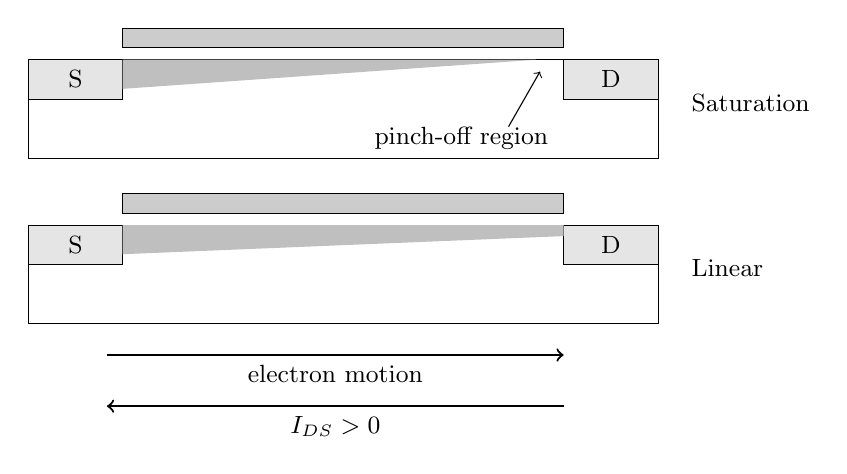
\begin{tikzpicture}[x=1cm,y=1cm,font=\small]
\foreach \y/\name in {0/Linear,2.1/Saturation}{
 \draw (0,\y) rectangle (8,\y+1.25);
 \draw[fill=gray!20] (0,\y+0.75) rectangle (1.2,\y+1.25);
 \draw[fill=gray!20] (6.8,\y+0.75) rectangle (8,\y+1.25);
 \draw[fill=gray!40] (1.2,\y+1.4) rectangle (6.8,\y+1.65);
 \draw (1.2,\y+1.25)--(6.8,\y+1.25);
 \node at (0.6,\y+1) {S};\node at (7.4,\y+1) {D};
 \node[anchor=west] at (8.3,\y+0.7) {\name};
}
\fill[gray!50] (1.2,1.25)--(6.8,1.25)--(6.8,1.11)--(1.2,0.88)--cycle;
\fill[gray!50] (1.2,3.35)--(6.45,3.35)--(1.2,2.98)--cycle;
\draw[->] (6.1,2.5)--(6.5,3.2);
\node at (5.5,2.35) {pinch-off region};
\draw[->,thick] (1,-0.4)--(6.8,-0.4) node[midway,below] {electron motion};
\draw[<-,thick] (1,-1.05)--(6.8,-1.05) node[midway,below] {$I_{DS}>0$};
\end{tikzpicture}
\end{latin}
\caption{نمای آموزشی کانال در دو ناحیه کاری، بر پایه شکل \secnum{۲.۳} کتاب.
کانال نزدیک \lr{Drain} بار کمتری دارد. در \lr{Saturation} حامل‌ها از ناحیه
\lr{Pinch-off} به \lr{Drain} انتقال می‌یابند \cite{weste}.}
\label{fig:mos-channel-shape}
\end{figure}

برای اختصار، \lr{Overdrive Voltage} را مطابق نماد کتاب به صورت
\(V_{GT}=V_{GS}-V_{tn}\) تعریف می‌کنیم. جدول \ref{tab:mos-regions} روند انتخاب
ناحیه را خلاصه می‌کند. در مدل قطعه‌ای، نقطه آستانه را با جریان صفر به
\lr{Cutoff} و مرز \lr{Linear} و \lr{Saturation} را به ناحیه دوم نسبت می‌دهیم.
دو رابطه جریان در مرز دوم یک مقدار می‌دهند.
\clearpage
\begin{table}[ht]
\centering
\caption{ناحیه‌های \lr{nMOS} با فرض \(V_{DS}\ge0\) و آستانه ثابت.}
\label{tab:mos-regions}
\begin{tabularx}{\textwidth}{rXX}
\toprule
ناحیه & شرط & تفسیر\\
\midrule
\lr{Cutoff} & \(V_{GS}\le V_{tn}\) & جریان صفر در مدل مرتبه اول\\
\lr{Linear} & \(V_{GS}>V_{tn},\ 0\le V_{DS}<V_{GT}\) & کانال تا دو انتها برقرار است\\
\lr{Saturation} & \(V_{GS}>V_{tn},\ V_{DS}\ge V_{GT}\) & جریان ایدئال با ولتاژ \lr{Gate} تعیین می‌شود\\
\bottomrule
\end{tabularx}
\end{table}

\subsection{مثال‌های تشخیص ناحیه با \lr{Source} غیرصفر}
در مثال‌های فرضی این قسمت، \(V_{tn}=\qty{0.4}{\volt}\) ثابت است.
اگر \(V_G=\qty{1.2}{\volt}\)، \(V_S=\qty{0.3}{\volt}\) و
\(V_D=\qty{0.5}{\volt}\) باشند، ابتدا اختلاف‌ها را حساب می‌کنیم
\[
 V_{GS}=1.2-0.3=\qty{0.9}{\volt},\qquad
 V_{DS}=0.5-0.3=\qty{0.2}{\volt},\qquad
 V_{GT}=0.9-0.4=\qty{0.5}{\volt}.
\]
چون \(V_{GS}>V_{tn}\) و \(0.2<0.5\)، ناحیه \lr{Linear} است.
از سوی دیگر \(V_{GD}=1.2-0.5=\qty{0.7}{\volt}>V_{tn}\) نیز همان نتیجه را تأیید می‌کند.

اگر تنها \(V_D\) به \qty{1.0}{\volt} تغییر کند، \(V_{DS}=\qty{0.7}{\volt}\)
و \(V_{GD}=\qty{0.2}{\volt}\) می‌شوند. شرط \(V_{DS}\ge V_{GT}\) برقرار است
و ترانزیستور در \lr{Saturation} قرار می‌گیرد. اگر در حالت دیگری
\(V_G=\qty{0.6}{\volt}\) باشد و \(V_S=\qty{0.3}{\volt}\) باقی بماند،
\(V_{GS}=\qty{0.3}{\volt}<V_{tn}\) و ترانزیستور در \lr{Cutoff} است.
شرط روشن‌شدن پیش از مقایسه \(V_{DS}\) با \(V_{GT}\) بررسی می‌شود.

برای \lr{Body} ثابت و \lr{Source} متحرک، آستانه واقعی می‌تواند با
\lr{Body Effect} تغییر کند. این سه مثال برای تمرین اختلاف ولتاژ، آستانه را
ثابت فرض کرده‌اند. تحلیل اثر بایاس \lr{Body} در دامنه بخش \secnum{۲.۴} است.
\subsection{ولتاژ تغذیه و محدودیت اکسید}
\(V_{DD}\) ولتاژ ریل تغذیه نسبت به \lr{GND} با مرجع صفر است.
اسلاید ۲۵، تغذیه \qty{5}{\volt} در مثال تاریخی دهه ۱۹۸۰ و کاهش ولتاژ در
فناوری‌های مورد بحث خود را نشان می‌دهد \cite{mos}.
با نازک‌شدن اکسید، همان اختلاف ولتاژ می‌تواند میدان عمودی بزرگ‌تری ایجاد کند.
در مدل یکنواخت، بزرگی میدان اکسید تقریباً \(E_{\mathrm{ox}}=V_{\mathrm{ox}}/t_{\mathrm{ox}}\)
است، که \(V_{\mathrm{ox}}\) ولتاژ دو سوی خود اکسید است.
انتخاب تغذیه باید با محدودیت افزاره و مشخصات فناوری سازگار باشد.
کاهش ولتاژ در رابطه توان دینامیکی، انرژی هر شارژ را کاهش می‌دهد.
هم‌زمان، جریان و زمان تغییر ولتاژ مدار نیز با نقطه بایاس تغییر می‌کنند.
این وابستگی، سرعت، توان و قابلیت اطمینان را به انتخاب مشترک ولتاژ مرتبط می‌کند.
\clearpage

\section{استخراج و کاربرد روابط \lr{Long-channel I-V}}
\label{sec:book-mos-current}
\subsection{فرض‌های مدل و معنای پارامترها}
مدل \lr{Long-channel} را \lr{Ideal}، \lr{First-order} یا \lr{Shockley Model}
نیز می‌نامند. کانال به اندازه‌ای بلند فرض می‌شود که مدل سرعت متناسب با میدان
طولی قابل‌استفاده باشد. \lr{Mobility}، ضخامت مؤثر اکسید و آستانه را در این تحلیل
ثابت می‌گیریم. جریان \lr{Gate} و جریان حالت خاموش صفر فرض می‌شوند. اثرهای
\lr{Velocity Saturation}، \lr{Mobility Degradation} و \lr{Channel Length Modulation}
در بخش \secnum{۲.۴} به تحلیل افزوده می‌شوند \cite[صفحات ۶۴ و ۶۵]{weste}.

در مدل کانال تدریجی، تغییر پتانسیل در امتداد کانال نسبت به تغییر عمودی آن آرام
فرض می‌شود. در نتیجه، بار موضعی را می‌توان با یک رابطه خازنی تقریب زد.
برای محاسبه حاضر، تأثیر تغییر بایاس محلی بر بار \lr{Depletion} در یک آستانه ثابت
خلاصه می‌شود. این فرض‌ها دامنه کاربرد روابط را تعیین می‌کنند.
نمادهای جدول \ref{tab:mos-parameters} پیش از استخراج به کار می‌روند.
\begin{table}[ht]
\centering
\caption{نمادها و واحدهای روابط جریان.}
\label{tab:mos-parameters}
\begin{tabularx}{\textwidth}{rXr}
\toprule
نماد & تعریف & واحد نمونه\\
\midrule
\(W,L\) & عرض کانال و طول مسیر میان \lr{Source} و \lr{Drain} & \unit{\metre}\\
\(t_{\mathrm{ox}}\) & ضخامت اکسید یا ضخامت معادل تعریف‌شده & \unit{\metre}\\
\(\varepsilon_{\mathrm{ox}}\) & \lr{Permittivity} اکسید & \unit{\farad\per\metre}\\
\(C_{\mathrm{ox}}\) & ظرفیت اکسید بر واحد سطح & \unit{\farad\per\metre\squared}\\
\(C_g\) & ظرفیت مدل صفحه‌ای \lr{Gate} و کانال & \unit{\farad}\\
\(\mu_n,\mu_p\) & \lr{Mobility} الکترون و \lr{Hole} & \unit{\metre\squared\per\volt\per\second}\\
\(\beta\) & ضریب فناوری و هندسه در رابطه جریان & \unit{\ampere\per\volt\squared}\\
\(V_{GT}\) & اضافه‌ولتاژ \(V_{GS}-V_{tn}\) در \lr{nMOS} & \unit{\volt}\\
\bottomrule
\end{tabularx}
\end{table}

\subsection{ظرفیت اکسید، هندسه و \lr{EOT}}
طول \(L\) در راستای حرکت حامل از \lr{Source} به \lr{Drain} و عرض \(W\)
در راستای عمود بر آن، روی سطح کانال اندازه‌گیری می‌شود.
در \lr{Strong Inversion}، \lr{Gate} و کانال در دو سوی عایق، تقریباً یک خازن
صفحه‌ای می‌سازند. مساحت مؤثر هندسی \(WL\) است و برای اکسید \lr{SiO\(_2\)} داریم
\begin{equation}
 \varepsilon_{\mathrm{ox}}=3.9\varepsilon_0,\qquad
 C_{\mathrm{ox}}=\frac{\varepsilon_{\mathrm{ox}}}{t_{\mathrm{ox}}},\qquad
 C_g=C_{\mathrm{ox}}WL.
 \label{eq:mos-oxide-cap}
\end{equation}
\(\varepsilon_0\approx\qty{8.85e-12}{\farad\per\metre}\) است.
در واحد سانتی‌متری کتاب، همین مقدار
\qty{8.85e-14}{\farad\per\centi\metre} نوشته می‌شود
\cite[رابطه \secnum{۲.۲}، شکل \secnum{۲.۶}]{weste}.
با نصف‌شدن ضخامت، ظرفیت بر واحد سطح دو برابر می‌شود. با دوبرابرشدن عرض، ظرفیت
کل دو برابر می‌شود. \(C_{\mathrm{ox}}\) و \(C_g\) واحد و نقش متفاوتی دارند.

برای نمونه فرضی \(t_{\mathrm{ox}}=\qty{10}{\nano\metre}\)،
\(W=\qty{1}{\micro\metre}\) و \(L=\qty{0.5}{\micro\metre}\)، ابتدا همه طول‌ها
را به متر می‌بریم. چون \(\qty{10}{\nano\metre}=10^{-8}\,\unit{\metre}\)، داریم
\begin{align*}
 C_{\mathrm{ox}}&=\frac{3.9(8.85\times10^{-12})}{10^{-8}}
 =3.4515\times10^{-3}\,\unit{\farad\per\metre\squared},\\
 C_g&=(3.4515\times10^{-3})(10^{-6})(0.5\times10^{-6})\,\unit{\farad}
 \approx\qty{1.73}{\femto\farad}.
\end{align*}
ضریب تبدیل مساحت از \unit{\micro\metre\squared} به \unit{\metre\squared}
برابر \(10^{-12}\) است، زیرا هر دو بعد در \(10^{-6}\) ضرب می‌شوند.
این ظرفیت صفحه‌ای، پایه استخراج جریان است. تقسیم آن میان پایانه‌ها در بخش
\secnum{۲.۳} بررسی می‌شود.

برای عایق \lr{High-k}، \lr{Equivalent Oxide Thickness} یا \lr{EOT} را ضخامت
لایه فرضی \lr{SiO\(_2\)} با همان \(C_{\mathrm{ox}}\) تعریف می‌کنند
\cite[صفحه ۶۶]{weste}. اگر ضخامت فیزیکی عایق \(t_h\) و گذردهی آن
\(\varepsilon_h\) باشد، از برابرگرفتن ظرفیت بر واحد سطح نتیجه می‌شود
\begin{equation}
 \frac{\varepsilon_h}{t_h}=\frac{\varepsilon_{\mathrm{ox}}}{\mathrm{EOT}}
 \quad\Longrightarrow\quad
 \mathrm{EOT}=t_h\frac{\varepsilon_{\mathrm{ox}}}{\varepsilon_h}.
 \label{eq:mos-eot}
\end{equation}
اگر گذردهی چهار برابر و ضخامت فیزیکی \qty{4}{\nano\metre} باشد،
\(\mathrm{EOT}=\qty{1}{\nano\metre}\) می‌شود. در این مثال، ضخامت فیزیکی بیشتر
با ظرفیت معادل همان اکسید نازک سازگار است.

\subsection{بار کانال در توضیح متوسط کتاب}
بار روی خازن به ولتاژ دو سوی همان خازن وابسته است. پتانسیل کانال میان
\(V_S\) و \(V_D\) تغییر می‌کند. کتاب برای استخراج مقدماتی، پتانسیل نماینده کانال
را میانگین دو انتها می‌گیرد و می‌نویسد
\begin{align}
 V_c&\approx\frac{V_S+V_D}{2}=V_S+\frac{V_{DS}}2,\notag\\
 V_{gc}&\approx V_G-V_c=V_{GS}-\frac{V_{DS}}2.
 \label{eq:mos-mean-potential}
\end{align}
برای تشکیل بار متحرک، ولتاژ باید از آستانه عبور کند. با تعریف بزرگی بار کانال
\(Q_{\mathrm{ch}}\ge0\)، رابطه مقدماتی کتاب چنین بازنویسی می‌شود
\begin{equation}
 Q_{\mathrm{ch}}\approx C_g(V_{gc}-V_{tn})
 \approx C_{\mathrm{ox}}WL\left(V_{GT}-\frac{V_{DS}}2\right).
 \label{eq:mos-average-charge}
\end{equation}
این توضیح از رابطه \secnum{۲.۱} کتاب و اسلاید ۱۵ گرفته شده است.
علامت بار الکترون‌ها منفی است. در این رابطه با بزرگی آن کار می‌کنیم.
افزایش \(V_{GS}\) بار متحرک را بیشتر می‌کند. افزایش \(V_{DS}\) با ثابت‌ماندن
\(V_{GS}\)، اضافه‌ولتاژ مؤثر نزدیک \lr{Drain} را کم می‌کند.

میانگین دو ولتاژ انتهایی یک ساده‌سازی برای استخراج مقدماتی است.
پتانسیل واقعی در طول کانال الزاماً خطی با مکان تغییر نمی‌کند، بنابراین
\eqref{eq:mos-average-charge} را به عنوان تقریب بزرگی کل بار به کار می‌بریم.
استخراج با بار موضعی در ادامه، همان رابطه جریان را در مدل کانال تدریجی به دست می‌دهد
و نیاز به فرض خطی‌بودن پتانسیل مکانی را برمی‌دارد.

\subsection{\lr{Mobility}، میدان طولی و زمان عبور}
\lr{Mobility} ضریب تبدیل بزرگی میدان الکتریکی به سرعت متوسط رانش در مدل میدان
کم است. اگر \(v\) بزرگی سرعت و \(E\) بزرگی میدان طولی باشد، داریم
\begin{equation}
 v=\mu_n E,\qquad E\approx\frac{V_{DS}}L,\qquad
 t_{\mathrm{tr}}\approx\frac Lv.
 \label{eq:mos-drift}
\end{equation}
رابطه‌های \secnum{۲.۳} و \secnum{۲.۴} کتاب و اسلاید ۱۶ همین مسیر را بیان می‌کنند.
\(t_{\mathrm{tr}}\) زمان عبور حامل در این تصویر مقدماتی است. تأخیر گیت به جریان
شارژ و تخلیه بار خارجی نیز وابسته است.

برای فهم واحد \(\mu\)، میدان واحد \unit{\volt\per\metre} دارد و سرعت واحد
\unit{\metre\per\second}. پس واحد ضریب تناسب
\unit{\metre\squared\per\volt\per\second} است. تبدیل واحد رایج کتاب چنین است
\begin{equation*}
 \qty{1}{\centi\metre\squared\per\volt\per\second}
 =10^{-4}\,\unit{\metre\squared\per\volt\per\second}.
\end{equation*}
کتاب برای الکترون در میدان کم حدود \num{500} تا
\qty{700}{\centi\metre\squared\per\volt\per\second}
را ذکر می‌کند و سپس کاهش \lr{Mobility} در میدان‌های قوی را یادآور می‌شود
\cite[صفحه ۶۶]{weste}. مقدار مناسب هر مثال باید از داده همان مثال برداشته شود.

در مثال فرضی \(L=\qty{1}{\micro\metre}\)، \(V_{DS}=\qty{0.1}{\volt}\)
و \(\mu_n=\qty{500}{\centi\metre\squared\per\volt\per\second}\)، داریم
\[
 E\approx\frac{0.1}{10^{-6}}=10^5\,\unit{\volt\per\metre},\qquad
 v\approx(0.05)(10^5)=\qty{5000}{\metre\per\second},\qquad
 t_{\mathrm{tr}}\approx\qty{0.2}{\nano\second}.
\]
در این محاسبه، تناسب سرعت با میدان و تقریب میدان متوسط فرض شده‌اند.

\subsection{استخراج رابطه \lr{Linear} با روش کتاب}
جریان، بار عبوری در واحد زمان است. در تصویر بار متوسط و زمان عبور متوسط،
جریان برابر \(Q_{\mathrm{ch}}/t_{\mathrm{tr}}\) تخمین زده می‌شود.
با جای‌گذاری \eqref{eq:mos-average-charge} و \eqref{eq:mos-drift}، مراحل حذف
عامل‌ها را به صورت زیر دنبال می‌کنیم
\begin{align}
 I_{DS}&\approx\frac{Q_{\mathrm{ch}}}{L/v}
 =Q_{\mathrm{ch}}\frac vL,\notag\\
 &\approx C_{\mathrm{ox}}WL\left(V_{GT}-\frac{V_{DS}}2\right)
 \frac{\mu_n V_{DS}}{L^2},\notag\\
 &=\mu_n C_{\mathrm{ox}}\frac WL
 \left(V_{GT}V_{DS}-\frac{V_{DS}^2}{2}\right).
 \label{eq:mos-book-linear}
\end{align}
از یک عامل \(L\) در صورت و دو عامل \(L\) در مخرج، نسبت \(1/L\) باقی می‌ماند.
با معرفی پارامتر فناوری \(k'_n\) و پارامتر فناوری و هندسه \(\beta_n\)، داریم
\begin{equation}
 k'_n=\mu_n C_{\mathrm{ox}},\qquad
 \beta_n=k'_n\frac WL=\mu_n C_{\mathrm{ox}}\frac WL.
 \label{eq:mos-beta}
\end{equation}
پس رابطه مدل برای \(V_{GS}>V_{tn}\) و \(0\le V_{DS}\le V_{GT}\) چنین است
\begin{equation}
 \boxed{I_{DS}=\beta_n\left[(V_{GS}-V_{tn})V_{DS}-\frac{V_{DS}^2}{2}\right].}
 \label{eq:mos-linear}
\end{equation}
این رابطه با روابط \secnum{۲.۵} تا \secnum{۲.۷} کتاب و اسلاید ۱۷ سازگار است.
علامت مساوی در \eqref{eq:mos-linear} بیانگر رابطه تعریف‌شده در مدل ایدئال است.

واحد \(\mu C_{\mathrm{ox}}\) برابر
\(\unit{\farad\per\volt\per\second}=\unit{\ampere\per\volt\squared}\) است.
نسبت \(W/L\) بی‌بعد است. داخل کروشه دو جمله با واحد \unit{\volt\squared}
داریم و حاصل، جریان با واحد \unit{\ampere} است.
برخی منابع، عامل \(1/2\) را در تعریف \(k'\) یا ضریب جریان جذب می‌کنند.
پانوشت صفحه ۶۶ کتاب نیز این تفاوت را یادآوری می‌کند.
پیش از استفاده از مقدار نقل‌شده، تعریف ضریب را با \eqref{eq:mos-beta} مقایسه می‌کنیم.

\subsection{استخراج تکمیلی با بار موضعی و انتگرال}
برای دقیق‌ترکردن استدلال در چارچوب همان مدل، مکان \(x\) را از \lr{Source}
در \(x=0\) تا \lr{Drain} در \(x=L\) تعریف می‌کنیم. \(V(x)\) پتانسیل محلی
نسبت به \lr{Source} است. پس \(V(0)=0\) و \(V(L)=V_{DS}\).
در قطعه کوچکی به طول \(dx\)، بزرگی بار متحرک کانال برابر است با
\begin{equation}
 dQ_{\mathrm{ch}}=W C_{\mathrm{ox}}[V_{GT}-V(x)]\,dx.
 \label{eq:mos-local-charge}
\end{equation}
عبارت \(C_{\mathrm{ox}}[V_{GT}-V(x)]\) بار بر واحد سطح و
\(Wdx\) سطح قطعه است. بار علامت‌دار الکترون‌ها، منفی این مقدار است.

زمان عبور از همین قطعه \(dt=dx/v(x)\) و بزرگی سرعت رانش
\(v(x)=\mu_n\,dV/dx\) است. این رابطه از بزرگی میدان استفاده می‌کند.
با تقسیم بار عبوری بر زمان و فرض جریان پایدار در طول کانال، داریم
\begin{equation}
 I_{DS}=W\mu_nC_{\mathrm{ox}}[V_{GT}-V(x)]\frac{dV}{dx}.
 \label{eq:mos-local-current}
\end{equation}
در جریان پایدار، بار در هیچ قطعه‌ای انباشته نمی‌شود، بنابراین جریان عبوری از
همه مقطع‌ها یکسان است. دو طرف را در \(dx\) ضرب و در طول کانال جمع می‌کنیم.
نماد انتگرال، جمع پیوسته سهم قطعه‌های کوچک است. با تغییر متغیر از مکان به
پتانسیل، جمع از صفر تا \(V_{DS}\) انجام می‌شود
\begin{equation*}
 \int_0^L I_{DS}\,dx
 =W\mu_nC_{\mathrm{ox}}\int_0^{V_{DS}}(V_{GT}-V)\,dV.
\end{equation*}
سمت چپ چون جریان ثابت است، \(I_{DS}L\) می‌شود. در سمت راست، مساحت زیر خط
\(V_{GT}-V\) در بازه صفر تا \(V_{DS}\)، مساحت یک مستطیل به ارتفاع \(V_{GT}\)
منهای مساحت مثلث به ارتفاع و قاعده \(V_{DS}\) است. پس
\begin{equation*}
 I_{DS}L=W\mu_n C_{\mathrm{ox}}
 \left(V_{GT}V_{DS}-\frac12V_{DS}^2\right).
\end{equation*}
تقسیم بر \(L\)، دقیقاً رابطه \eqref{eq:mos-linear} را در فرض‌های مدل به دست
می‌دهد. عامل یک‌دوم از تغییر بار در امتداد کانال ناشی می‌شود. شرط
\(V_{DS}\le V_{GT}\) تضمین می‌کند بار موضعی در سراسر کانال نامنفی باقی بماند.

\subsection{تقریب مقاومتی و مرز \lr{Saturation}}
برای \(V_{DS}\ll V_{GT}\)، جمله مربعی نسبت به جمله اول کوچک است. نسبت بزرگی
آن دو جمله \(V_{DS}/(2V_{GT})\) است. با حذف جمله کوچک، داریم
\begin{equation}
 I_{DS}\approx\beta_nV_{GT}V_{DS},\qquad
 R_{\mathrm{on}}\approx\frac{V_{DS}}{I_{DS}}
 \approx\frac1{\beta_nV_{GT}}.
 \label{eq:mos-small-vds}
\end{equation}
مقاومت تقریبی با ولتاژ \lr{Gate} کنترل می‌شود.
در رابطه کامل ناحیه \lr{Linear}، نسبت \(V_{DS}/I_{DS}\) برابر
\(1/[\beta_n(V_{GT}-V_{DS}/2)]\) است و با ولتاژ تغییر می‌کند.

برای \(\beta_n=\qty{200}{\micro\ampere\per\volt\squared}\)،
\(V_{GT}=\qty{0.8}{\volt}\) و \(V_{DS}=\qty{0.1}{\volt}\)، جریان کامل
به صورت زیر محاسبه می‌شود.
\[
 200[0.8(0.1)-0.1^2/2]=\qty{15}{\micro\ampere}.
\]
تقریب مقاومتی \qty{16}{\micro\ampere} می‌دهد، حدود \num{6.7} درصد بیشتر از مقدار
رابطه کامل. برای کاهش خطای این تقریب باید نسبت \(V_{DS}/V_{GT}\) کوچک‌تر شود.

در مرز تشکیل \lr{Pinch-off}، \(V_{GD}=V_{tn}\)، بنابراین ولتاژ اشباع در مدل
بلندکانال برابر است با
\begin{equation}
 V_{DS,\mathrm{sat}}=V_{GT}=V_{GS}-V_{tn}.
 \label{eq:mos-vdsat}
\end{equation}
با جای‌گذاری همین مقدار در \eqref{eq:mos-linear}، داریم
\begin{align}
 I_{DS,\mathrm{sat}}
 &=\beta_n\left(V_{GT}^2-\frac{V_{GT}^2}{2}\right)
 =\frac{\beta_n}{2}V_{GT}^2,\notag\\
 &\boxed{I_{DS,\mathrm{sat}}=\frac{\beta_n}{2}(V_{GS}-V_{tn})^2.}
 \label{eq:mos-saturation}
\end{align}
این رابطه برای \(V_{GS}>V_{tn}\) و \(V_{DS}\ge V_{DS,\mathrm{sat}}\) به کار
می‌رود \cite[رابطه \secnum{۲.۸} و اسلاید ۱۸]{weste,mos}.
پس از مرز، افزایش ولتاژ \lr{Drain} عمدتاً روی ناحیه نزدیک \lr{Drain} می‌افتد.
در تقریبِ طول مؤثر ثابت، جریان به مقدار مرزی محدود می‌شود.

می‌توان رابطه \lr{Linear} را با کامل‌کردن مربع نیز بازنوشت
\begin{equation}
 I_{DS}=\frac{\beta_n}{2}
 \left[V_{GT}^2-(V_{GT}-V_{DS})^2\right],\qquad 0\le V_{DS}\le V_{GT}.
 \label{eq:mos-complete-square}
\end{equation}
در مرز، مربع دوم صفر و جریان برابر بیشینه این قطعه است.
برای \(V_{DS}>V_{GT}\)، فرض بار نامنفی تا انتهای کانال از اعتبار می‌افتد و
قطعه اشباع انتخاب می‌شود. همین انتخاب از افت مصنوعی جریان ناشی از ادامه‌دادن
سهمی به بیرون بازه جلوگیری می‌کند.

\subsection{رابطه قطعه‌ای، پیوستگی و جریان‌های \lr{Ion} و \lr{Ioff}}
برای \(V_{DS}\ge0\)، مدل جریان را با شرط‌ها یکجا می‌نویسیم
\begin{equation}
 I_{DS}=\begin{cases}
 0,&V_{GS}\le V_{tn},\\[2pt]
 \beta_n(V_{GT}V_{DS}-V_{DS}^2/2),
 &V_{GS}>V_{tn},\quad 0\le V_{DS}<V_{GT},\\[2pt]
 \beta_n V_{GT}^2/2,
 &V_{GS}>V_{tn},\quad V_{DS}\ge V_{GT}.
 \end{cases}
 \label{eq:mos-piecewise}
\end{equation}
این صورت، مرزهای رابطه \secnum{۲.۱۰} کتاب و اسلاید ۱۹ را نیز پوشش می‌دهد.
در \(V_{DS}=0\)، قطعه \lr{Linear} جریان صفر می‌دهد. در
\(V_{DS}=V_{GT}\)، دو قطعه مقدار \(\beta_n V_{GT}^2/2\) می‌دهند.
با \(V_{GS}\) نزدیک آستانه از بالا، جریان اشباع به صفر میل می‌کند.
در هر سه بررسی، رفتار قطعه‌ای پیوسته است.

کتاب \(I_{\mathrm{on}}\) را جریان در \(V_{GS}=V_{DS}=V_{DD}\)، و
\(I_{\mathrm{off}}\) را جریان در \(V_{GS}=0,V_{DS}=V_{DD}\) تعریف می‌کند.
برای \(V_{DD}>V_{tn}>0\)، شرط اشباع برای حالت روشن برقرار است و داریم
\begin{equation}
 I_{\mathrm{on}}=\frac{\beta_n}{2}(V_{DD}-V_{tn})^2,\qquad
 I_{\mathrm{off}}=0\quad\text{\rl{در مدل مرتبه اول}}.
 \label{eq:mos-ion-ioff}
\end{equation}
اگر \(V_{DD}\le V_{tn}\) باشد، همین مدل جریان حالت روشن را نیز صفر می‌گیرد.
این شرط پیش از مربع‌کردن اختلاف بررسی می‌شود. جریان خاموش واقعی در درس
\lr{Leakage} تحلیل خواهد شد \cite[رابطه \secnum{۲.۹}]{weste}.

در \lr{Saturation}، دوبرابرشدن \(W\) با بقیه پارامترهای ثابت، جریان را دو برابر
می‌کند. دوبرابرشدن \(L\) جریان را نصف می‌کند، مشروط به حفظ اعتبار مدل و پارامترها.
دوبرابرشدن \(V_{GT}\) جریان را چهار برابر می‌کند. برای تغییر \(V_{GS}\)،
ابتدا آستانه را کم می‌کنیم و سپس توان دو می‌گیریم.
\clearpage

\subsection{حل مثال اسلاید ۲۰ با واحدهای سازگار}
داده‌های اسلاید ۲۰ عبارت‌اند از \(t_{\mathrm{ox}}=\qty{10}{\nano\metre}\)،
\(\mu_n=\qty{350}{\centi\metre\squared\per\volt\per\second}\)،
\(V_{tn}=\qty{0.7}{\volt}\) و \(W/L=4/2=2\) \cite{mos}.
در اسلاید، ضخامت به صورت \(100\) \lr{angstrom} داده شده است.
هر \lr{angstrom} برابر \(10^{-10}\,\unit{\metre}\) است، پس
\(100\) \lr{angstrom} برابر \qty{10}{\nano\metre} می‌شود.

با واحد متر، \(\mu_n=0.035\,\unit{\metre\squared\per\volt\per\second}\)
و \(C_{\mathrm{ox}}=3.4515\times10^{-3}\,\unit{\farad\per\metre\squared}\) است.
بنابراین
\begin{align*}
 k'_n&=(0.035)(3.4515\times10^{-3})\,
 \unit{\ampere\per\volt\squared}
 \approx\qty{120.8}{\micro\ampere\per\volt\squared},\\
 \beta_n&=k'_n\frac WL\approx\qty{241.6}{\micro\ampere\per\volt\squared}.
\end{align*}
اسلاید ضریب \(k'_n\) را حدود \qty{120}{\micro\ampere\per\volt\squared}
گزارش می‌کند. برای هماهنگی با دقت همان مثال، در ادامه
\(\beta_n=\qty{240}{\micro\ampere\per\volt\squared}\) می‌گیریم.
وقتی \(V_{GS}=\qty{3}{\volt}\)، اضافه‌ولتاژ \(V_{GT}=\qty{2.3}{\volt}\) است.
برای \(V_{DS}=\qty{1}{\volt}\)، ناحیه \lr{Linear} و جریان
\[
 I_{DS}=240\left[2.3(1)-\frac{1^2}{2}\right]\,\unit{\micro\ampere}
 =\qty{432}{\micro\ampere}
\]
می‌شود. برای \(V_{DS}=\qty{4}{\volt}\)، ناحیه \lr{Saturation} و جریان
\[
 I_{DS}=\frac{240}{2}(2.3)^2\,\unit{\micro\ampere}
 =\qty{634.8}{\micro\ampere}\approx\qty{0.635}{\milli\ampere}
\]
است. مقدار \(V_{DS}=\qty{2.3}{\volt}\) در هر دو فرمول همین پاسخ را می‌دهد.
منحنی‌های شکل \ref{fig:mos-slide-curves} با همین ضریب گرد‌شده محاسبه شده‌اند.

\begin{figure}[ht]
\centering
\begin{latin}
\PersianMathDigits
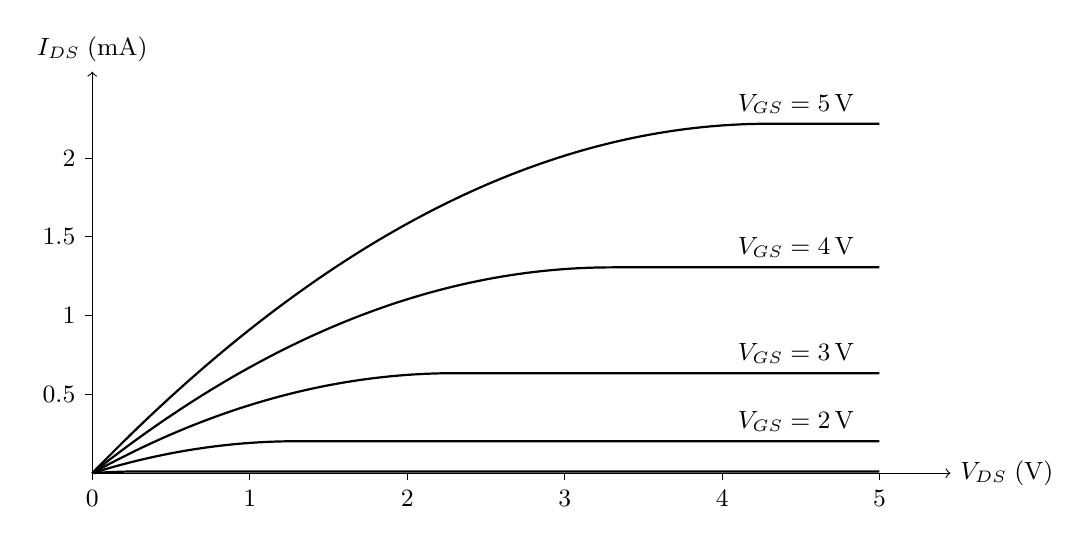
\begin{tikzpicture}[x=2cm,y=2cm,font=\small]
\draw[->] (0,0)--(5.45,0) node[right] {$V_{DS}\;(\mathrm V)$};
\draw[->] (0,0)--(0,2.55) node[above] {$I_{DS}\;(\mathrm{mA})$};
\foreach \x in {0,1,2,3,4,5}{\draw (\x,0)--(\x,-0.045) node[below] {$\x$};}
\foreach \y in {0.5,1,1.5,2}{\draw (0,\y)--(-0.045,\y) node[left] {$\y$};}
\foreach \g in {1,2,3,4,5}{
 \draw[thick,domain=0:5,samples=101] plot (\x,{0.24*((\g-0.7)*min(\x,\g-0.7)-0.5*min(\x,\g-0.7)^2)});
}
\node[anchor=south east] at (4.9,2.22) {$V_{GS}=5\,\mathrm V$};
\node[anchor=south east] at (4.9,1.307) {$V_{GS}=4\,\mathrm V$};
\node[anchor=south east] at (4.9,0.635) {$V_{GS}=3\,\mathrm V$};
\node[anchor=south east] at (4.9,0.203) {$V_{GS}=2\,\mathrm V$};
\end{tikzpicture}
\end{latin}
\caption{مشخصه‌های محاسبه‌شده از مدل \lr{Long-channel} با داده اسلاید ۲۰ و
\(\beta_n=\qty{240}{\micro\ampere\per\volt\squared}\). منحنی \(V_{GS}=0\)
روی محور افقی است و پایین‌ترین منحنی غیرصفر به \(V_{GS}=\qty{1}{\volt}\) مربوط است.
نمودار، بازتولید مدل ایدئال با فرض‌های بیان‌شده است \cite{mos}.}
\label{fig:mos-slide-curves}
\end{figure}

\subsection{حل مثال \texorpdfstring{\secnum{۲.۱}}{۲.۱} کتاب و اختلاف عدد ضریب}
در مثال \secnum{۲.۱} کتاب، نام فناوری \qty{65}{\nano\metre} است، اما طول رسم‌شده
\(L=\qty{50}{\nano\metre}\) و \(W=\qty{100}{\nano\metre}\) داده شده است.
برای محاسبه \(W/L\)، ابعاد واقعی داده‌شده را به کار می‌بریم. سایر داده‌ها
\(t_{\mathrm{ox}}=\qty{1.05}{\nano\metre}\)،
\(\mu_n=\qty{80}{\centi\metre\squared\per\volt\per\second}\) و
\(V_{tn}=\qty{0.3}{\volt}\) در دمای ذکرشده \qty{70}{\degreeCelsius} هستند
\cite[صفحه ۶۷]{weste}.

تبدیل‌ها \(\mu_n=0.008\,\unit{\metre\squared\per\volt\per\second}\)،
\(t_{\mathrm{ox}}=1.05\times10^{-9}\,\unit{\metre}\) و \(W/L=2\) می‌دهند.
پس با ثابت \(\varepsilon_0\) درج‌شده در کتاب داریم
\begin{align}
 C_{\mathrm{ox}}&=\frac{3.9(8.85\times10^{-12})}{1.05\times10^{-9}}
 \approx0.03287\,\unit{\farad\per\metre\squared},\notag\\
 k'_n&\approx(0.008)(0.03287)
 \approx\qty{263}{\micro\ampere\per\volt\squared},\notag\\
 \beta_n&\approx\qty{526}{\micro\ampere\per\volt\squared}.
 \label{eq:mos-book-beta}
\end{align}
در رابطه \secnum{۲.۱۱} چاپ کتاب، ضریب پیش از \(W/L\) برابر
\qty{262}{\micro\ampere\per\volt\squared} نوشته شده است.
محاسبه از داده‌های درج‌شده حدود \qty{263}{\micro\ampere\per\volt\squared}
می‌دهد. اختلاف حدود \num{0.4} درصد است. برای سازگاری داخلی، جدول و نمودار این جزوه
همگی با \(\beta_n=\qty{526}{\micro\ampere\per\volt\squared}\) محاسبه شده‌اند.

برای \(V_{GS}=0\) و \qty{0.2}{\volt}، شرط روشن‌شدن برقرار نیست.
برای چهار مقدار بعدی، جدول \ref{tab:mos-book-points} ولتاژ مرزی و جریان اشباع
را نشان می‌دهد. مثلاً در \(V_{GS}=\qty{0.8}{\volt}\)،
\(V_{GT}=\qty{0.5}{\volt}\) و جریان اشباع
\((526/2)(0.5)^2=\qty{65.75}{\micro\ampere}\) است.
\begin{table}[ht]
\centering
\caption{نقاط مرزی مثال کتاب، با ضریب محاسبه‌شده و گرد‌شده در \eqref{eq:mos-book-beta}.}
\label{tab:mos-book-points}
\begin{tabular}{ccc}
\toprule
\(V_{GS}\;(\unit{\volt})\)&\(V_{DS,\mathrm{sat}}\;(\unit{\volt})\)&
\(I_{DS,\mathrm{sat}}\;(\unit{\micro\ampere})\)\\
\midrule
\(0.4\)&\(0.1\)&\(2.63\)\\
\(0.6\)&\(0.3\)&\(23.67\)\\
\(0.8\)&\(0.5\)&\(65.75\)\\
\(1.0\)&\(0.7\)&\(128.87\)\\
\bottomrule
\end{tabular}
\end{table}

برای رسم هر منحنی، از صفر تا \(V_{DS,\mathrm{sat}}\) رابطه \lr{Linear} و پس از
آن رابطه \lr{Saturation} به کار می‌رود. شکل \ref{fig:mos-book-curves} نتیجه را
نمایش می‌دهد. افزاره کوچک این مثال، از نظر فیزیکی اثرهای میدان قوی دارد.
کتاب صریحاً استفاده از مدل ایدئال را برای این تمرین خواسته و اثرهای اصلاحی را
به بخش بعد ارجاع داده است.
\begin{figure}[ht]
\centering
\begin{latin}
\PersianMathDigits
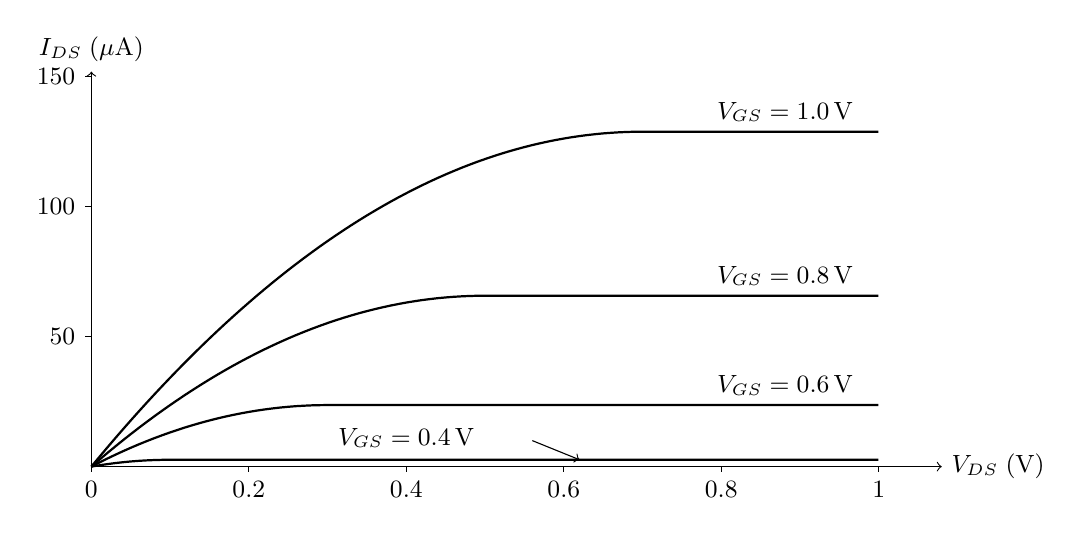
\begin{tikzpicture}[x=10cm,y=0.033cm,font=\small]
\draw[->] (0,0)--(1.08,0) node[right] {$V_{DS}\;(\mathrm V)$};
\draw[->] (0,0)--(0,152) node[above] {$I_{DS}\;(\mathrm{\mu A})$};
\foreach \x in {0,0.2,0.4,0.6,0.8,1}{\draw (\x,0)--(\x,-2) node[below] {$\x$};}
\foreach \y in {50,100,150}{\draw (0,\y)--(-0.008,\y) node[left] {$\y$};}
\foreach \g in {0.4,0.6,0.8,1.0}{
 \draw[thick,domain=0:1,samples=101] plot (\x,{526*((\g-0.3)*min(\x,\g-0.3)-0.5*min(\x,\g-0.3)^2)});
}
\node[anchor=south east] at (0.98,128.87) {$V_{GS}=1.0\,\mathrm V$};
\node[anchor=south east] at (0.98,65.75) {$V_{GS}=0.8\,\mathrm V$};
\node[anchor=south east] at (0.98,23.67) {$V_{GS}=0.6\,\mathrm V$};
\draw[->] (0.56,10)--(0.62,2.63);
\node at (0.40,11) {$V_{GS}=0.4\,\mathrm V$};
\end{tikzpicture}
\end{latin}
\caption{منحنی‌های مدل ایدئال مثال \secnum{۲.۱} کتاب با
\(\beta_n=\qty{526}{\micro\ampere\per\volt\squared}\).
دو منحنی \(V_{GS}=0\) و \(V_{GS}=\qty{0.2}{\volt}\) روی محور افقی قرار دارند
\cite[شکل \secnum{۲.۷}]{weste}.}
\label{fig:mos-book-curves}
\end{figure}

\subsection{\lr{pMOS} با بزرگی مثبت و سپس قرارداد علامت‌دار}
برای \lr{pMOS}، \lr{Source} پایانه پرپتانسیل‌تر است. آستانه علامت‌دار را
\(V_{tp}<0\) و بزرگی مثبت آن را \(V_{TP}=|V_{tp}|\) می‌نامیم.
ولتاژها و ضریب مثبت را به صورت زیر تعریف می‌کنیم
\begin{equation}
 V_{SG}=V_S-V_G,\quad V_{SD}=V_S-V_D,\quad
 V_{GT,p}=V_{SG}-V_{TP},\quad
 \beta_p=\mu_p C_{\mathrm{ox}}\frac{W_p}{L_p}>0.
 \label{eq:mos-p-defs}
\end{equation}
با این تعریف، برای \(V_{SD}\ge0\)، بزرگی جریان از \lr{Source} به \lr{Drain}
دقیقاً همان ساختار مدل \lr{nMOS} را دارد
\cite[صفحه ۶۷ و اسلایدهای ۲۱ و ۲۲]{weste,mos}.
\begin{equation}
 |I_{DS,p}|=\begin{cases}
 0,&V_{SG}\le V_{TP},\\[2pt]
 \beta_p(V_{GT,p}V_{SD}-V_{SD}^2/2),
 &V_{SG}>V_{TP},\quad 0\le V_{SD}<V_{GT,p},\\[2pt]
 \beta_p V_{GT,p}^2/2,
 &V_{SG}>V_{TP},\quad V_{SD}\ge V_{GT,p}.
 \end{cases}
 \label{eq:mos-p-piecewise}
\end{equation}
در قرارداد جریان \lr{Drain}-به-\lr{Source}، مقدار جریان \lr{pMOS} منفی است.
همچنین \(V_{GS}=-V_{SG}\) و \(V_{DS}=-V_{SD}\) هستند.
بنابراین نمودار علامت‌دار کتاب در ربع سوم قرار می‌گیرد.
برای نوشتن رابطه علامت‌دار اشباع با \(\beta_p>0\)، می‌توان نوشت
\begin{equation}
 I_{DS,p}=-\frac{\beta_p}{2}(V_{GS}-V_{tp})^2,
 \quad V_{GS}<V_{tp},\quad V_{SD}\ge V_{GT,p}.
 \label{eq:mos-p-signed}
\end{equation}
کتاب برای ساده‌کردن محاسبه‌ها اغلب بزرگی‌ها را به کار می‌برد.
در هر مسئله، قرارداد بزرگی یا علامت‌دار باید در تمام رابطه ثابت بماند.

مثال فرضی \(V_S=\qty{1.8}{\volt}\)، \(V_G=\qty{0.6}{\volt}\)،
\(V_D=\qty{1.5}{\volt}\)، \(V_{tp}=-\qty{0.4}{\volt}\) و
\(\beta_p=\qty{100}{\micro\ampere\per\volt\squared}\) را در نظر بگیرید.
\(V_{SG}=\qty{1.2}{\volt}\)، \(V_{GT,p}=\qty{0.8}{\volt}\) و
\(V_{SD}=\qty{0.3}{\volt}\) هستند. پس ناحیه \lr{Linear} و جریان
\[
 |I_{DS,p}|=100\left[0.8(0.3)-\frac{0.3^2}{2}\right]\,\unit{\micro\ampere}
 =\qty{19.5}{\micro\ampere}
\]
است. در قرارداد علامت‌دار، \(V_{DS}=-\qty{0.3}{\volt}\) و
\(I_{DS,p}=-\qty{19.5}{\micro\ampere}\) می‌شوند.
اگر تنها \(V_D\) به \qty{0.6}{\volt} کاهش یابد، \(V_{SD}=\qty{1.2}{\volt}\)
و ناحیه \lr{Saturation} است. بزرگی جریان
\((100/2)(0.8)^2=\qty{32}{\micro\ampere}\) خواهد بود.

در نمونه \lr{pMOS} همراه شکل \secnum{۲.۷} کتاب، هندسه و بزرگی آستانه با نمونه
\lr{nMOS} یکسان و \(\mu_p=\mu_n/2\) است. پس در ولتاژهای متناظر، بزرگی جریان
نصف می‌شود. مثلاً نقطه \((V_{DS},I_{DS})=(\qty{1}{\volt},\qty{128.87}{\micro\ampere})\)
در نمونه \lr{nMOS} متناظر با حدود
\((-\qty{1}{\volt},-\qty{64.44}{\micro\ampere})\) در نمونه \lr{pMOS} است.

\clearpage
\subsection{نسبت \lr{Mobility} و انتخاب عرض \lr{pMOS}}
برای دو ترانزیستور با \(L\)، \(C_{\mathrm{ox}}\) و اضافه‌ولتاژ یکسان، برابرشدن
جریان در مدل نیازمند \(\beta_p=\beta_n\) است. از \eqref{eq:mos-beta} داریم
\begin{equation}
 \mu_pW_p=\mu_nW_n
 \quad\Longrightarrow\quad
 \frac{W_p}{W_n}=\frac{\mu_n}{\mu_p}.
 \label{eq:mos-width-ratio}
\end{equation}
اسلاید ۲۲ مقادیر \(\mu_n=350\) و \(\mu_p=120\) را برای نمونه فناوری خود ذکر
می‌کند. نسبت این دو حدود \num{2.92} است. همان اسلاید برای مثال‌های کلاس، نسبت ۲ را
به عنوان فرض قراردادی اعلام می‌کند. کتاب نیز نسبت متداول ۲ تا ۳ را بیان کرده و
برای مثال‌هایش معمولاً ۲ می‌گیرد. پس با داده عددی ۳۵۰ و ۱۲۰، عرض حدود \num{2.92} برابر
و با فرض قراردادی ۲، عرض دو برابر به دست می‌آید.
\(\mu\)های این پاراگراف واحد مشترک
\unit{\centi\metre\squared\per\volt\per\second} دارند.

اگر طول یا ظرفیت اکسید یا اضافه‌ولتاژها برابر نباشند، باید از خود رابطه جریان
استفاده کرد. برای اشباع و اضافه‌ولتاژهای مثبت، برابرشدن جریان‌ها می‌دهد
\begin{equation}
 \frac{W_p}{W_n}
 =\frac{\mu_nC_{\mathrm{ox},n}}{\mu_pC_{\mathrm{ox},p}}
 \frac{L_p}{L_n}\left(\frac{V_{GT,n}}{V_{GT,p}}\right)^2.
 \label{eq:mos-general-width}
\end{equation}
بنابراین نسبت عرض از فرض‌های فیزیکی و نقطه بایاس مسئله نتیجه می‌شود.
\clearpage

\subsection{تحلیل مدار مقاومتی و انتخاب ریشه فیزیکی}
در مدار شکل \ref{fig:mos-load}، \lr{Source} و \lr{Body} به زمین،
\lr{Drain} از طریق \(R_D\) به \(V_{DD}\) و \lr{Gate} به ولتاژ ثابت \(V_G\)
متصل‌اند. برای مثال آموزشی، \(V_{DD}=\qty{1.8}{\volt}\)،
\(V_G=\qty{1.2}{\volt}\)، \(V_{tn}=\qty{0.4}{\volt}\) و
\(\beta_n=\qty{1}{\milli\ampere\per\volt\squared}\) هستند.
\begin{figure}[ht]
\centering
\begin{latin}
\begin{circuitikz}[font=\small]
\draw (0,0) node[nmos] (M) {};
\draw (M.S)--++(0,-0.4) node[ground] {};
\draw (M.D) to[R,l=$R_D$] ++(0,2) node[vcc] {$V_{DD}$};
\draw (M.G)--++(-1,0) node[ocirc] {} node[left] {$V_G$};
\draw (M.D)--++(1,0) node[ocirc] {} node[right] {$V_D=V_{DS}$};
\end{circuitikz}
\end{latin}
\caption{مدار آموزشی برای پیوند رابطه ترانزیستور با قانون جریان و ولتاژ مدار.
اتصال \lr{Body} به زمین در نماد به صورت ضمنی فرض شده است.}
\label{fig:mos-load}
\end{figure}

ابتدا اضافه‌ولتاژ گیت را محاسبه می‌کنیم.
\[
 V_{GT}=1.2-0.4=\qty{0.8}{\volt}.
\]
از افت ولتاژ مقاومت و برابری جریان مقاومت با جریان ترانزیستور داریم
\begin{equation}
 I_{DS}=\frac{V_{DD}-V_D}{R_D}.
 \label{eq:mos-load-line}
\end{equation}
برای \(R_D=\qty{2}{\kilo\ohm}\)، ابتدا اشباع را فرض می‌کنیم.
جریان پیشنهادی و ولتاژ متناظر با آن چنین‌اند.
\[
 \begin{aligned}
 I_{DS}&=(1/2)(0.8)^2=\qty{0.32}{\milli\ampere},\\
 V_D&=1.8-(0.32)(2)=\qty{1.16}{\volt}.
 \end{aligned}
\]
در این ضرب، \unit{\milli\ampere} در \unit{\kilo\ohm} واحد \unit{\volt} می‌دهد.
چون \(1.16\ge0.8\)، شرط اشباع برقرار و فرض تأیید می‌شود.

اکنون \(R_D=\qty{5}{\kilo\ohm}\) را بگذارید. فرض اشباع همان جریان
\qty{0.32}{\milli\ampere} را می‌دهد. ولتاژ متناظر با این فرض برابر است با
\[
 V_D=1.8-(0.32)(5)=\qty{0.2}{\volt}.
\]
چون \(0.2<0.8\)، این فرض با شرط ناحیه سازگار نیست.
با فرض \lr{Linear} و نوشتن جریان در \unit{\milli\ampere} و ولتاژ در \unit{\volt}،
رابطه مقاومت و ترانزیستور را برابر می‌کنیم
\begin{align}
 \frac{1.8-V_D}{5}&=0.8V_D-\frac{V_D^2}{2},\notag\\
 0.36-0.2V_D&=0.8V_D-0.5V_D^2,\notag\\
 0.5V_D^2-V_D+0.36&=0.
 \label{eq:mos-load-quadratic}
\end{align}
اعداد رابطه \eqref{eq:mos-load-quadratic} در دستگاه واحد معرفی‌شده نوشته شده‌اند.
برای معادله \(aV_D^2+bV_D+c=0\)، فرمول ریشه
به صورت زیر است.
\[
 V_D=\frac{-b\pm\sqrt{b^2-4ac}}{2a}.
\]
با \(a=0.5,b=-1,c=0.36\)، داخل رادیکال \(1-0.72=0.28\) می‌شود، پس
\begin{equation*}
 V_D=1\pm\sqrt{0.28},\qquad
 V_{D,1}\approx\qty{0.471}{\volt},\qquad
 V_{D,2}\approx\qty{1.529}{\volt}.
\end{equation*}
شرط ناحیه انتخاب‌شده \(0\le V_D<\qty{0.8}{\volt}\) است.
فقط ریشه \qty{0.471}{\volt} این شرط را دارد. ریشه دوم از ادامه ریاضی رابطه
\lr{Linear} به بیرون بازه معتبر آن به دست آمده است. با ریشه پذیرفته‌شده،
جریان چنین محاسبه می‌شود.
\[
 I_{DS}=\frac{1.8-0.47085}{5}\approx\qty{0.266}{\milli\ampere}.
\]
جای‌گذاری در رابطه ترانزیستور نیز همین جریان را می‌دهد.

\subsection{تمرین‌های پاسخ‌دار و مرور تحلیلی}
\textbf{تمرین ۱.} با \(V_G=\qty{0.8}{\volt}\)، \(V_S=\qty{0.5}{\volt}\)،
\(V_D=\qty{1.2}{\volt}\) و آستانه ثابت \qty{0.4}{\volt}، جریان مدل چیست؟
\(V_{GS}=0.8-0.5=\qty{0.3}{\volt}\) و کمتر از آستانه است.
پس در مدل مرتبه اول \(I_{DS}=0\)، هرچند ولتاژ \lr{Drain} مثبت است.

\textbf{تمرین ۲.} برای \(\beta_n=\qty{200}{\micro\ampere\per\volt\squared}\)،
\(V_{tn}=\qty{0.4}{\volt}\)، \(V_{GS}=\qty{1.2}{\volt}\) و
\(V_{DS}=\qty{0.2}{\volt}\)، ناحیه و جریان را بیابید.
\(V_{GT}=\qty{0.8}{\volt}\) و \(0.2<0.8\)، پس \lr{Linear} است.
جریان از رابطه \lr{Linear} به دست می‌آید.
\[
 200[0.8(0.2)-0.2^2/2]=\qty{28}{\micro\ampere}.
\]

\textbf{تمرین ۳.} در تمرین قبل، \(V_{DS}=\qty{1}{\volt}\) شود.
اکنون \(1\ge0.8\)، پس اشباع برقرار است. جریان برابر است با
\[
 I_{DS}=(200/2)(0.8)^2=\qty{64}{\micro\ampere}.
\]
اگر اشتباهاً رابطه \lr{Linear} را ادامه دهیم، \qty{60}{\micro\ampere} می‌دهد.
این عدد شرط اعتبار همان فرمول را نقض می‌کند.

\textbf{تمرین ۴.} در اشباع، \(I_{DS}=\qty{36}{\micro\ampere}\)،
\(\beta_n=\qty{200}{\micro\ampere\per\volt\squared}\) و
\(V_{tn}=\qty{0.4}{\volt}\) است. \(V_{GS}\) را بیابید.
ابتدا مربع اضافه‌ولتاژ را از رابطه جریان جدا می‌کنیم.
\[
 (V_{GS}-0.4)^2=\frac{2(36)}{200}=0.36\,\unit{\volt\squared}.
\]
ریشه‌ها \(V_{GS}=0.4\pm0.6\) هستند.
شرط \(V_{GS}>V_{tn}\)، پاسخ \(V_{GS}=\qty{1}{\volt}\) را انتخاب می‌کند.
برای معتبرماندن فرض اشباع، \(V_{DS}\ge\qty{0.6}{\volt}\) نیز لازم است.

\textbf{تمرین ۵.} در فرض اشباع، \(V_{tn}=\qty{0.3}{\volt}\) و سایر پارامترها
ثابت باشند. کاهش \(V_{GS}\) از \qty{1}{\volt} به \qty{0.8}{\volt}
جریان را در چه نسبتی تغییر می‌دهد؟
اضافه‌ولتاژها \qty{0.7}{\volt} و \qty{0.5}{\volt} هستند، بنابراین
\[
 \frac{I_2}{I_1}=\frac{(0.8-0.3)^2}{(1-0.3)^2}
 =\frac{0.25}{0.49}\approx0.510.
\]
جریان حدود ۴۹ درصد کاهش می‌یابد. مربعِ نسبت اضافه‌ولتاژها در رابطه ظاهر می‌شود.

\textbf{تمرین ۶.} اگر \(W\) و \(L\) هر دو دو برابر شوند، با سایر شرایط ثابت،
جریان این مدل چه تغییری می‌کند؟ نسبت \(W/L\) ثابت و در نتیجه \(\beta\)
و جریان ثابت می‌مانند. مدل صفحه‌ای، \(C_g\propto WL\)، ظرفیت را چهار برابر می‌دهد.
برای استنباط تأخیر مدار باید اثر بار و جریان همه مراحل بررسی شود.

\textbf{تمرین ۷.} با \(\mu_n/\mu_p=2\)، طول برابر، اکسید برابر و بزرگی آستانه
برابر، جریان متناظر \lr{pMOS} با عرض برابر نسبت به \lr{nMOS} چقدر است؟
\(\beta_p/\beta_n=1/2\)، پس در اضافه‌ولتاژ و ناحیه متناظر، بزرگی جریان نصف است.
عرض دو برابر \lr{pMOS}، ضریب‌ها را در همین فرض‌ها برابر می‌کند.

\textbf{تمرین ۸.} برای \lr{pMOS} با \(V_S=\qty{1.2}{\volt}\)،
\(V_G=\qty{1.0}{\volt}\)، \(V_D=\qty{0.2}{\volt}\) و
\(V_{tp}=-\qty{0.3}{\volt}\)، ناحیه چیست؟
\(V_{SG}=\qty{0.2}{\volt}<|V_{tp}|\)، پس \lr{Cutoff} است.
بزرگی زیاد \(V_{SD}\) شرط روشن‌شدن را تأمین نمی‌کند.

\textbf{تمرین ۹.} در مثال اسلاید، با \(\beta_n=\qty{240}{\micro\ampere\per\volt\squared}\)،
\(V_{GS}=\qty{5}{\volt}\) و \(V_{DS}=\qty{5}{\volt}\)، جریان و ناحیه را بیابید.
اضافه‌ولتاژ گیت برابر است با
\[
 V_{GT}=5-0.7=\qty{4.3}{\volt}.
\]
پس اشباع برقرار است و محاسبه جریان می‌دهد
\[
 (240/2)(4.3)^2=\qty{2218.8}{\micro\ampere}\approx\qty{2.22}{\milli\ampere}.
\]
این نتیجه با منحنی بالای شکل \ref{fig:mos-slide-curves} سازگار است.

\textbf{تمرین ۱۰.} چرا در مرز \(V_{DS}=V_{GT}\) دو فرمول جریان برابرند؟
در قطعه \lr{Linear}، جای‌گذاری می‌دهد
\[
 \beta_n(V_{GT}^2-V_{GT}^2/2)=\beta_nV_{GT}^2/2.
\]
این دقیقاً مقدار قطعه اشباع است. بنابراین نحوه نسبت‌دادن خود نقطه مرزی به یکی
از دو ناحیه، مقدار جریان را تغییر نمی‌دهد.

در حل مسئله، مسیر محاسبه از تعریف اختلاف ولتاژ آغاز می‌شود، سپس شرط روشن‌شدن،
مرز ناحیه و مقدار جریان بررسی می‌شوند. اگر ولتاژ یا جریان مجهول از معادله مدار
به دست آید، نتیجه باید دوباره در شرط ناحیه جای‌گذاری شود.
این روند، ریشه ریاضی را به پاسخ سازگار با مدل فیزیکی تبدیل می‌کند.
\clearpage

\section{مشخصه‌های ظرفیت و ولتاژ، \lr{C-V}}
\label{sec:book-cv}
در مدل تفصیلی این بخش، پسوند \(i\) سهم \lr{Intrinsic} و پسوند
\(\mathrm{ov}\) سهم \lr{Overlap} را مشخص می‌کند.
\(C_0=WLC_{\mathrm{ox}}\) ظرفیت هندسی مرجع است.
نماد بدون این پسوندها، در مدار معادل کامل، مجموع سهم‌های دو پایانه مربوط را
نشان می‌دهد. ظرفیت مؤثر گذار، علاوه بر بایاس به حرکت پایانه دیگر نیز وابسته است.
\BookletSubsections{notes/booklet-01/ch2-capacitance-basics}
\BookletSubsections{notes/booklet-01/ch2-gate-capacitance}
\BookletSubsections{notes/booklet-01/ch2-diffusion-capacitance}
\BookletReview{notes/booklet-01/final-review}

